% ==================================================
% 第四章　實驗方法與結果分析
% ==================================================
\chapter{實驗方法與結果分析}
\label{c:experiments}

本章針對所提出之全身預測控制方法進行實驗設計與分析，
評估執行動態模型、動態導航、底盤與手臂協同操作，
以及住宅場景中的任務銜接。
首先說明實驗環境、比較條件與評估指標，
再依序分析模型預測、導航避障及操作追蹤表現，
最後討論整合任務、計算效能與方法限制。

% ==================================================
% 4.1 實驗環境與評估指標
% ==================================================
\section{實驗環境與評估指標}
\label{sec:experimental_setup_metrics}

實驗由模型預測、導航控制與操作任務三個層次展開，
分別觀察命令執行特性、障礙交會及機構操作對系統表現的影響。
各項比較採用明確的起始條件、控制設定與評估區間，
並區分運動追蹤、任務完成及計算成本，
作為後續結果分析的共同基準。

% ==================================================
% 4.1.1 實驗平台與場景配置
% ==================================================
\subsection{實驗平台與場景配置}
\label{subsec:experimental_platform_scenarios}

本研究以四輪十字配置之全向底盤與 Lite 6 六軸手臂
構成移動操作平台，並配置平行夾爪、二維雷射與影像感測。
軟體透過 ROS 2 Jazzy
進行感測、規劃與控制模組之間的資料交換\cite{macenski2022ros2}。
移動操作與住宅任務使用 NVIDIA Isaac Sim
建立物理模擬環境\cite{nvidiaisaacsim}；
動態導航方法比較另使用 Gazebo Harmonic，
各項結果依其實際平台與控制設定分別呈現。

住宅整合任務之主要時間與命令設定如
\cref{tab:ch4_execution_settings}所示。
物理步長為 $0.01$ s，控制週期為 $0.05$ s，
每個控制週期對應五個物理更新步。
手臂位置設定點由設定點變化率逐步積分，
再由關節位置控制器追蹤；
底盤命令則經平滑、防護與輪級限制後作用於平台。
預測步數與控制權重依比較目的設定，於各節列示。

\begin{table}[htbp]
    \centering
    \caption{住宅整合實驗之主要執行設定}
    \label{tab:ch4_execution_settings}
    \begingroup
    \small
    \renewcommand{\arraystretch}{1.2}
    \begin{tabular}{p{0.30\textwidth} p{0.60\textwidth}}
        \hline
        項目 & 設定 \\
        \hline
        機器人平台 & 四輪全向底盤、六軸 Lite 6 與平行夾爪 \\
        物理步長 $\Delta t_p$ & $0.01$ s \\
        控制週期 $\Delta t$ & $0.05$ s \\
        在途命令長度 & $8$ 個物理步，對應 $0.08$ s \\
        手臂位置控制增益 & 各軸 $k_p=600$、$k_d=60$ \\
        影像解析度 & $640\times480$ 像素 \\
        視覺辨識 & 六類目標之 Mask R-CNN 實例分割 \\
        \hline
    \end{tabular}
    \endgroup
\end{table}

場景依實驗目的分為動態導航、獨立抽屜操作與住宅整合任務。
動態導航場景配置固定障礙與移動障礙，
用於觀察交會、減速及側向避讓。
抽屜場景提供具有固定滑軌方向的操作目標，
用於比較預測時域與移動、停駐策略。
住宅場景沿用第二章介紹的室內配置，
包含臥室、客廳、右側操作區及其間的通行空間，
並配置門扇、茶几、抽屜櫃與車尾收納盒。
主要空間與操作設備的相對位置如
\cref{fig:ch4_residential_scene_layout}所示。
門扇位於臥室與客廳之間，茶几取物區位於客廳，
抽屜操作區則設於右側房間，
使任務同時包含狹窄通行、室內導航及家具附近的協同操作。

\begin{figure}[htbp]
    \centering
    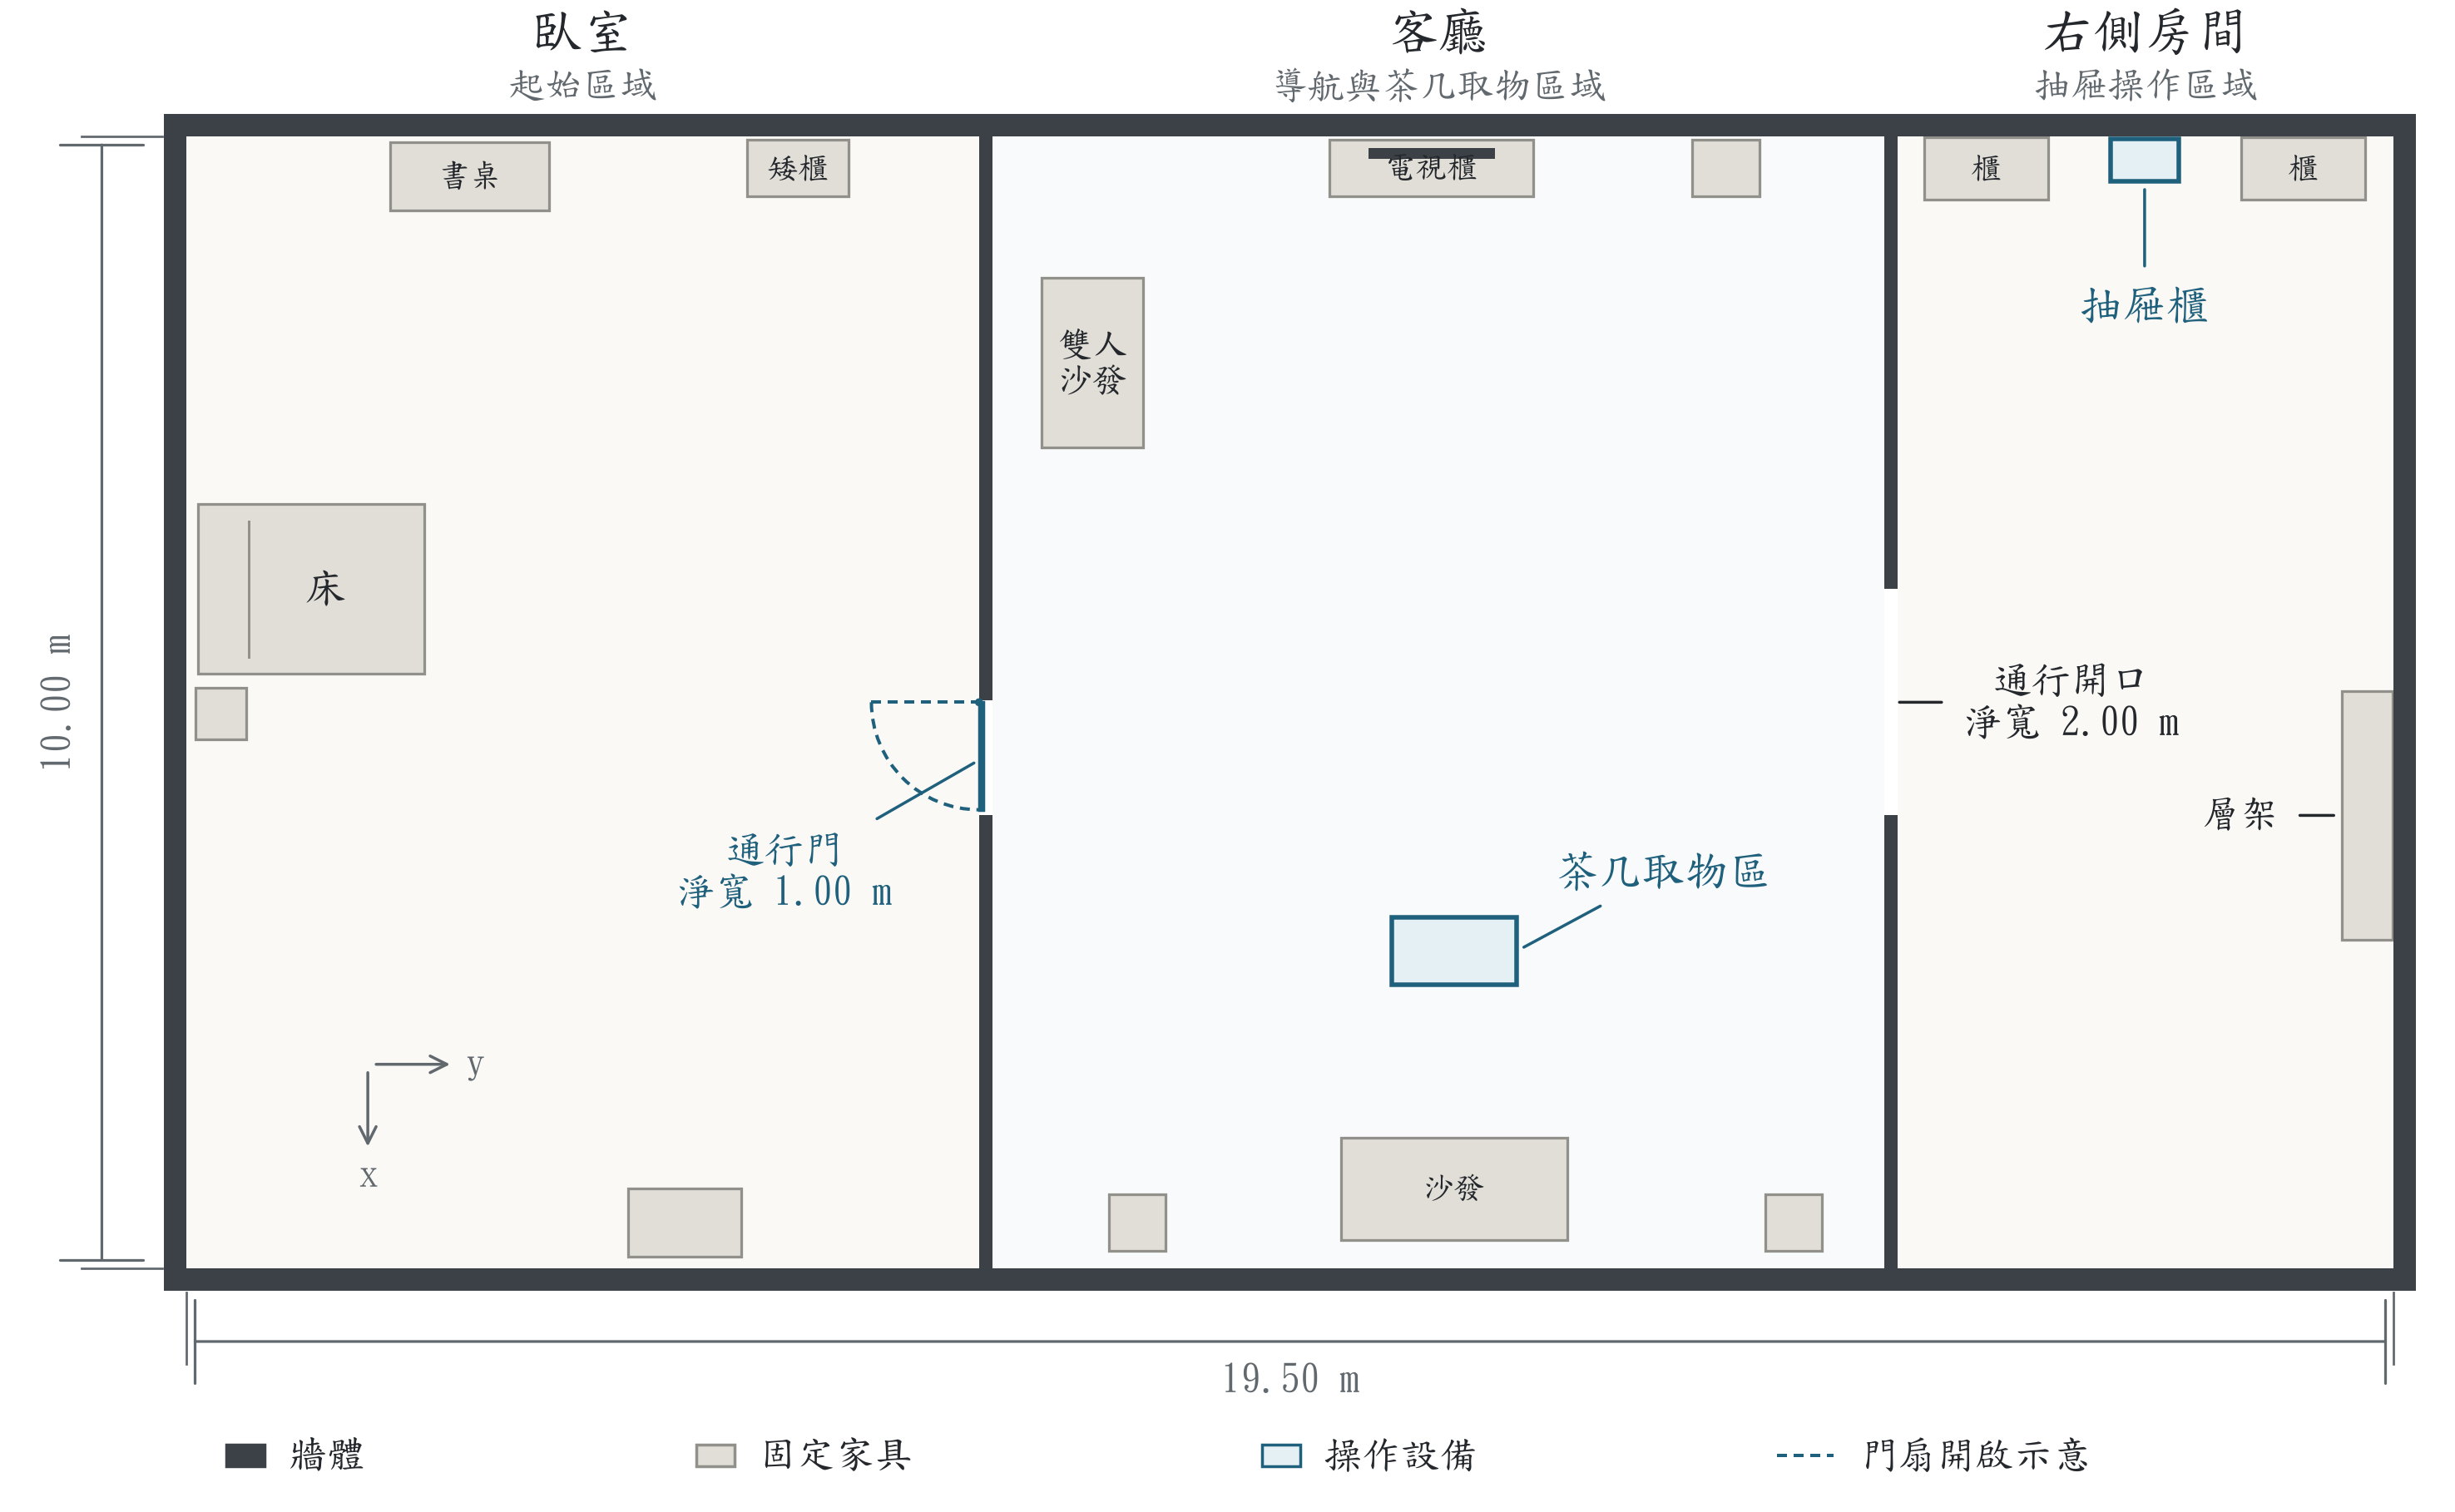
\includegraphics[width=0.98\textwidth]{figsrc/ch02/simulation_environment_map.png}
    \caption{住宅整合任務之場景配置與主要操作區域，
    包含臥室起始區域、通行門、客廳茶几取物區與右側房間抽屜操作區。}
    \label{fig:ch4_residential_scene_layout}
\end{figure}

住宅任務涵蓋開門通行、圓柱移動中抓取與收納、
開抽屜取筆與關閉抽屜，以及回程通行、關門與返回起點。
家具區域與物件類型作為任務輸入，
精確操作目標則由視覺量測與幾何估測建立。
環境配置、操作目標與移動障礙條件依各項實驗分別設定。

底盤位姿與關節狀態用於控制及軌跡分析，
視覺資料則保留影像擷取時間與相機位姿，
使目標估測、控制命令及實際運動能對齊至相同時間基準。
住宅整合任務的運動時間以模擬時鐘計算，
感知、規劃與求解耗時則以主機時間量測。
其餘比較的時間來源於對應小節說明。
控制週期與計算耗時分別呈現，
用於分析控制更新是否滿足實際命令生效期限。

% ==================================================
% 4.1.2 比較方法與控制條件
% ==================================================
\subsection{比較方法與控制條件}
\label{subsec:baseline_methods_control_conditions}

比較內容依研究目的分為執行模型、導航方法、
預測時域與操作策略，如\cref{tab:ch4_comparison_design}所示。
模型比較檢查設定點追蹤動態對預測誤差的影響；
導航比較評估障礙交會下的到達、接觸與時間表現；
操作比較則觀察底盤與手臂協同運動對末端追蹤及任務銜接的影響。

\begin{table}[htbp]
    \centering
    \caption{實驗比較項目與評估重點}
    \label{tab:ch4_comparison_design}
    \begingroup
    \small
    \renewcommand{\arraystretch}{1.25}
    \begin{tabular}{p{0.19\textwidth} p{0.35\textwidth} p{0.34\textwidth}}
        \hline
        比較項目 & 比較內容 & 評估重點 \\
        \hline
        執行動態模型
        & 直接速度積分模型與設定點增廣模型
        & 關節單步及多步預測誤差 \\

        導航控制方法
        & 本研究導航方法、Nav2 MPPI 與 RPP
        & 到達、障礙接觸、路徑與時間成本 \\

        避障模組
        & 控制屏障與原始雷射防護之啟用組合
        & 模組對通行與避障表現的影響 \\

        預測時域
        & 單步與多步全身預測控制
        & 末端誤差、命令變化與計算成本 \\

        操作策略
        & 移動中協同操作與停駐後操作
        & 操作追蹤、階段銜接與完整任務時間 \\
        \hline
    \end{tabular}
    \endgroup
\end{table}

導航基線採用 Nav2 系統提供的控制方法\cite{macenski2020nav2}。
比較時使用共同路線與對應障礙條件，
並列明速度、命令變化與機器人外形設定；
各方法可使用的運動方向依其控制形式說明。
避障消融則比較 CBF 與原始雷射防護的不同啟用組合，
觀察兩者在控制求解與命令執行端的作用。

模型辨識資料與驗證資料依時間區分，
各模型使用相同起始狀態及對應輸入歷程，
並在相同預測時間長度下計算誤差。
延遲前推、偏置估測及目標補償的啟用條件分別列示，
以說明各機制對預測與末端追蹤的影響。

預測時域比較採用相同的狀態與命令定義，
並列明預測步數、控制週期、終端權重與成本累加方式。
移動與停駐策略則以共同的任務起終條件比較，
同時分析接近、操作、退出及返回階段的時間，
使完整任務耗時能對應至實際運動與階段銜接。

% ==================================================
% 4.1.3 誤差、平順性與任務表現指標
% ==================================================
\subsection{誤差、平順性與任務表現指標}
\label{subsec:tracking_smoothness_task_metrics}

評估指標涵蓋預測誤差、末端追蹤、
命令平順性、任務完成與計算效能。
令 $t_j$ 為評估區間內的取樣時間，
$p_E^d(t_j)$、$R_E^d(t_j)$ 為目標末端位姿，
$p_E(t_j)$、$R_E(t_j)$ 為由實際構型計算的末端位姿。
位置與姿態追蹤誤差定義為
\begin{equation}
    \begin{aligned}
        e_p(t_j)
        &=\|p_E^d(t_j)-p_E(t_j)\|_2,\\
        e_R(t_j)
        &=\left\|
        \left[\log\!\left(R_E(t_j)^\top R_E^d(t_j)\right)\right]^\vee
        \right\|_2.
    \end{aligned}
    \label{eq:ch4_tcp_tracking_metrics}
\end{equation}
位置誤差以毫米表示，姿態誤差由弧度轉換為度。
控制追蹤誤差與視覺目標定位誤差分別計算，
以區分目標估測與運動執行對結果的影響。

對第 $r$ 個關節，給定預測時間長度 $\tau$，
以預測關節位置與對應時刻的實際位置計算
\begin{equation}
    e_{q,r}(t_j;\tau)
    =\hat q_{a,r}(t_j+\tau\mid t_j)-q_{a,r}(t_j+\tau).
    \label{eq:ch4_joint_prediction_error}
\end{equation}
各關節與各預測時間長度分別統計，
用於分析誤差隨預測時域增加的變化。
對選定誤差量 $e$，其均方根誤差為
\begin{equation}
    \operatorname{RMSE}(e)
    =\sqrt{\frac{1}{M}\sum_{j=1}^{M}\|e(t_j)\|_2^2},
    \label{eq:ch4_rmse}
\end{equation}
其中 $M$ 為評估區間的有效取樣數。
各類誤差另列第 $95$ 百分位數與最大值，
並依接近、機構操作及持物等階段分別分析。

命令平順性以實際放行輸入在共同取樣間隔 $\delta t$ 下的差分評估：
\begin{equation}
    a_{B,j}^{\mathrm{cmd}}
    =\frac{\xi_{B,j}^{\mathrm{appl}}-\xi_{B,j-1}^{\mathrm{appl}}}{\delta t},
    \qquad
    \dot u_{a,j}^{\mathrm{appl}}
    =\frac{u_{a,j}^{\mathrm{appl}}-u_{a,j-1}^{\mathrm{appl}}}{\delta t}.
    \label{eq:ch4_applied_command_variation}
\end{equation}
底盤平移、偏航及手臂各軸分別統計，
並觀察命令反轉與接近上限的情形。
實際運動平順性則由位姿與關節量測另行評估，
使命令變化與平台響應具有明確對應。

任務時間由共同起始事件計算至預定完成條件：
\begin{equation}
    T_{\mathrm{task}}=t_{\mathrm{end}}-t_{\mathrm{start}},
    \qquad
    \eta_T=
    \frac{T_{\mathrm{baseline}}-T_{\mathrm{proposed}}}
         {T_{\mathrm{baseline}}}\times100\%.
    \label{eq:ch4_task_time_comparison}
\end{equation}
$\eta_T$ 表示相對於比較策略的時間縮短比例。
局部操作時間與完整任務時間分別呈現，
並配合末端到位、機構位置、物件收納及返回條件
判定各階段與整體任務的完成情形。

導航表現另以到達情形、路徑長度、
最小障礙淨空與非任務指定接觸評估。
計算效能則記錄 QP 求解、整體控制更新及視覺處理耗時，
列出其中位數、第 $95$ 百分位數、最大值與逾時情形。
各項結果採用對應的評估區間與完成條件，
共同分析精度、運動連續性與任務效率。

% ==================================================
% 4.2 執行動態模型之辨識與預測驗證
% ==================================================
\section{執行動態模型之辨識與預測驗證}
\label{sec:execution_model_validation}

全身控制器需由輸入命令預測未來的底盤與手臂構型，
其中手臂的位置命令介面包含設定點累積與關節追蹤兩個過程。
本節先以自由空間運動紀錄辨識手臂追蹤模型，
再比較直接速度積分與設定點增廣模型的預測誤差，
最後分析命令生效延遲與等效偏置對狀態預測的影響。
辨識與重播計算分別沿用各組資料取得時的控制條件，
參數及誤差均對應其所屬的評估資料。

% ==================================================
% 4.2.1 手臂追蹤動態參數辨識
% ==================================================
\subsection{手臂追蹤動態參數辨識}
\label{subsec:arm_tracking_parameter_identification}

辨識資料包含六軸關節位置、實際寫入的位置設定點及物理時間戳記。
關節位置 $q_a^j$ 與設定點 $s_a^j$ 以同一物理步配對，
其中 $s_a^j$ 為作用於第 $j$ 至 $j+1$ 步的位置目標。
資料中的物理步長為 $0.01$ s，
上游控制命令每 $0.05$ s 更新，
設定點則於每一物理步依實際放行的變化率累積。
此時間關係使設定點追蹤能以第 3.2 節的逐步模型描述，
並將控制更新頻率與設定點積分頻率分別處理。

使用連續運動資料的前半段估計參數，後半段進行預測驗證。
對每個關節，以設定點與實際位置之差作為迴歸輸入，
以相鄰物理步的關節位移作為輸出，
依式\eqref{eq:ch3_arm_parameter_identification}
估計追蹤係數 $\hat\alpha_r$ 與每步偏置 $\hat b_r$。
驗證期間固定已辨識的參數，
使後續誤差反映模型對不同時間區段的預測能力。

各軸辨識結果如\cref{tab:ch4_arm_identification_parameters}所示。
為便於比較響應速度，另由離散追蹤係數換算等效時間常數：
\begin{equation}
    \tau_r=-\frac{\Delta t_p}{\ln(1-\hat\alpha_r)}.
    \label{eq:ch4_arm_equivalent_time_constant}
\end{equation}
此換算對應設定點固定時的指數衰減形式。
六軸的 $\hat\alpha_r$ 皆約為 $0.095$，
等效時間常數約為 $0.100$ s，
表示關節對設定點的追蹤會跨越數個控制週期持續進行。

\begin{table}[htbp]
    \centering
    \caption{自由空間資料之手臂追蹤動態辨識結果}
    \label{tab:ch4_arm_identification_parameters}
    \begingroup
    \small
    \renewcommand{\arraystretch}{1.2}
    \begin{tabular}{c c c c}
        \hline
        關節 & $\hat\alpha_r$ & $\hat b_r$（mrad/步） & $\tau_r$（ms） \\
        \hline
        1 & $0.095010$ & $1.194\times10^{-3}$  & $100.169$ \\
        2 & $0.095038$ & $2.715\times10^{-1}$  & $100.138$ \\
        3 & $0.095008$ & $-2.056\times10^{-2}$ & $100.171$ \\
        4 & $0.094992$ & $3.299\times10^{-3}$  & $100.189$ \\
        5 & $0.095013$ & $1.607\times10^{-4}$  & $100.166$ \\
        6 & $0.095019$ & $1.957\times10^{-5}$  & $100.159$ \\
        \hline
    \end{tabular}
    \endgroup
\end{table}

各軸的偏置量具有不同大小與方向。
以第二關節為例，設定點固定時的等效穩態偏移
$\hat b_2/\hat\alpha_2$ 約為 $2.856$ mrad；
因此，每步偏置須經追蹤動態累積後，才對應至固定設定點下的穩態差異。
在後半段資料的 $10$ ms 單物理步驗證中，
最大逐軸 RMSE 約為 $0.111$ mrad。
此結果用於描述該辨識條件下的位置介面響應，
後續再透過較長時間的預測，觀察誤差的累積情形。
控制增益、工具配置或負載改變時，
則以對應資料重新檢查參數與預測殘差。

% ==================================================
% 4.2.2 直接速度積分與增廣模型之比較
% ==================================================
\subsection{直接速度積分與增廣模型之比較}
\label{subsec:direct_augmented_model_comparison}

直接速度積分模型將設定點變化率視為關節速度，
由起始位置與區間內命令積分預測關節位置：
\begin{equation}
    \hat q_a^{\mathrm{dir}}(t+\tau\mid t)
    =q_a(t)+\int_t^{t+\tau}u_a^{\mathrm{appl}}(\lambda)\,\mathrm d\lambda.
    \label{eq:ch4_direct_velocity_prediction}
\end{equation}
離散計算時依物理步的實際命令作用區間對齊積分。
設定點增廣模型則由同一時刻的實際關節位置與設定點開始，
逐步推進設定點與關節追蹤狀態。
兩者均使用相同的驗證區段、預測起點與對應命令歷程。

首先比較一個控制週期，即 $50$ ms 的預測。
增廣模型分別採用逐步實錄設定點，
以及將整個預測區間的實際輸入平均後保持固定兩種重播方式。
前者保留區間內完整的設定點變化，
後者用於觀察輸入簡化對模型預測的影響。
兩種方式皆使用已記錄的後續輸入資訊，
評估範圍為已知輸入歷程下的離線條件預測。

\cref{tab:ch4_arm_prediction_rmse}列出與控制週期對齊之起點所得的結果。
直接速度積分的各軸 RMSE 約為 $24.988$--$25.378$ mrad，
採用實錄設定點的增廣模型則為 $0.001$--$0.444$ mrad。
改用區間平均輸入時，增廣模型的誤差為 $0.403$--$0.555$ mrad，
顯示保留設定點狀態與追蹤動態，可減少直接積分所產生的預測落差。
其中實錄設定點與區間平均輸入的差異，
亦反映控制區間內命令變化對短時預測的影響。

\begin{table}[htbp]
    \centering
    \caption{控制週期對齊之 $50$ ms 關節預測 RMSE（mrad）}
    \label{tab:ch4_arm_prediction_rmse}
    \begingroup
    \small
    \renewcommand{\arraystretch}{1.25}
    \begin{tabular}{c c c c}
        \hline
        關節 & 直接速度積分
        & \shortstack{增廣模型\\實錄設定點}
        & \shortstack{增廣模型\\區間平均輸入} \\
        \hline
        1 & $25.283$ & $0.010$ & $0.422$ \\
        2 & $25.075$ & $0.444$ & $0.555$ \\
        3 & $25.378$ & $0.035$ & $0.403$ \\
        4 & $24.988$ & $0.042$ & $0.406$ \\
        5 & $25.082$ & $0.003$ & $0.405$ \\
        6 & $25.275$ & $0.001$ & $0.417$ \\
        \hline
    \end{tabular}
    \endgroup
\end{table}

\cref{fig:ch4_arm_prediction_validation}(a)比較各軸誤差，
並以對數縱軸呈現不同量級。
為觀察預測時間增加時的變化，
另由驗證區段選取可涵蓋完整 $250$ ms 的共同起點，
分別計算 $10$、$50$、$100$、$150$ 與 $250$ ms 的預測誤差。
各時域均以實錄輸入逐步重播，
並以六軸中最大的逐軸 RMSE 作為比較量，
結果如\cref{fig:ch4_arm_prediction_validation}(b)所示。
共同起點使曲線的變化可對應至預測時間長度，
避免因評估區段不同而混入額外差異。
在 $250$ ms 時，直接速度積分與實錄設定點增廣模型的
最大逐軸 RMSE 分別約為 $102.868$ 與 $0.954$ mrad，
顯示兩者的預測差異隨評估時間延長而持續存在。

\begin{figure}[htbp]
    \centering
    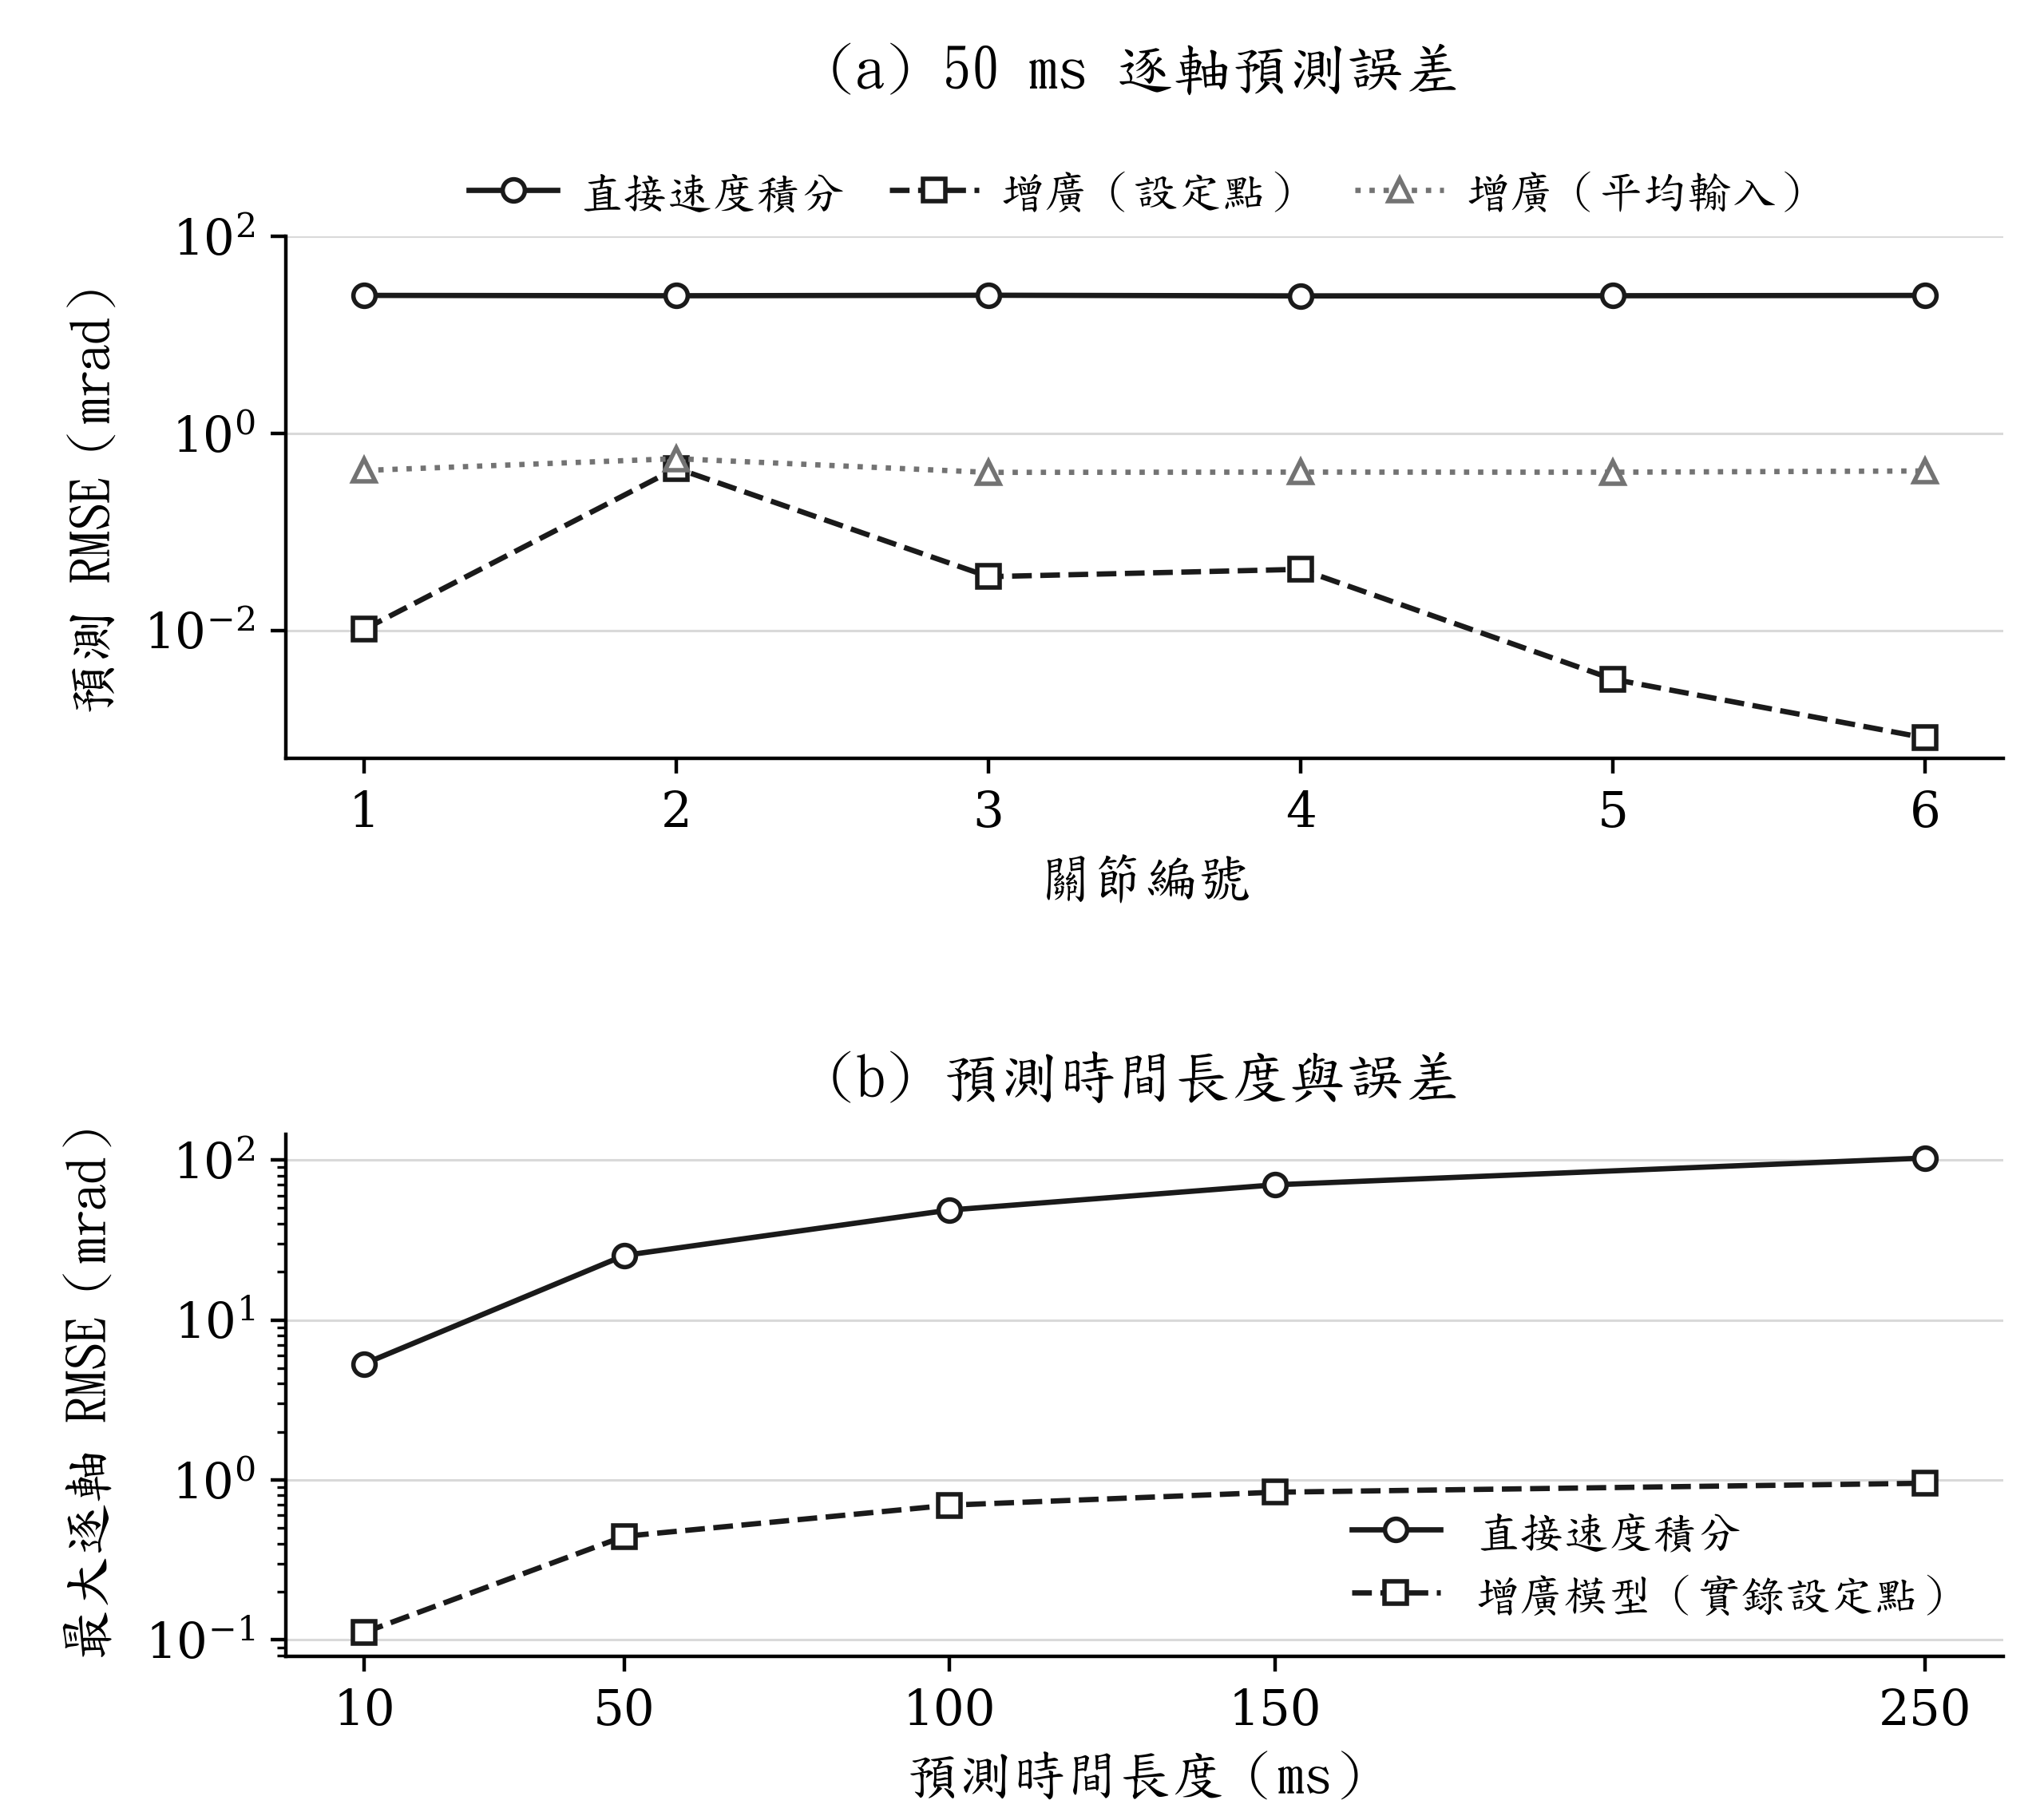
\includegraphics[width=0.98\textwidth]{figsrc/ch04/arm_model_prediction_validation.png}
    \caption{手臂執行模型之離線預測比較：
    (a) 控制週期對齊之 $50$ ms 逐軸 RMSE；
    (b) 共同起點下，不同預測時間長度的最大逐軸 RMSE。
    兩圖縱軸皆採對數尺度；區間平均輸入由該區間的實錄命令計算。}
    \label{fig:ch4_arm_prediction_validation}
\end{figure}

增廣模型能保留控制開始前已累積的設定點追蹤運動。
依本組辨識係數合成五個物理步後，
$A_q$ 與 $A_s$ 的對角元素分別約為 $0.607$ 與 $0.393$，
而設定點變化率對當期關節位置的直接係數約為 $0.00864$ s。
因此，一個控制週期內的關節位移同時取決於既有設定點差與新輸入，
其作用可由增廣狀態共同描述。
離線重播提供執行模型的預測依據，
線上控制的末端追蹤與任務表現則於後續協同操作實驗分析。

% ==================================================
% 4.2.3 命令延遲與偏置估測之影響
% ==================================================
\subsection{命令延遲與偏置估測之影響}
\label{subsec:delay_bias_effects}

模型預測除需符合關節追蹤特性，亦需對應命令實際生效時刻。
令 $t_s$ 為控制狀態的擷取時間，
$t_{\mathrm{pub}}$ 為候選命令發布時間，
$t_{\mathrm{act}}$ 為該命令首次作用於平台的時間，
狀態至生效延遲可分解為
\begin{equation}
    \tau_{\mathrm{sa}}
    =t_{\mathrm{act}}-t_s
    =(t_{\mathrm{pub}}-t_s)
     +(t_{\mathrm{act}}-t_{\mathrm{pub}}).
    \label{eq:ch4_command_activation_delay}
\end{equation}
利用 ROS 命令傳遞紀錄的來源序號，
可將求解端發布與執行端首次套用的事件逐筆配對。
自由空間紀錄中，各配置的狀態至生效延遲中位數介於 $60$--$80$ ms，
觀測到的最大值為 $140$ ms，皆以模擬時間計算。
此延遲量測對應命令傳遞時序，主機上的求解耗時另於第 4.6 節分析。

狀態取得至命令生效之間，平台仍會沿既有排程持續運動。
因此，第 3.7 節的在途命令前推保留底盤速度與設定點追蹤歷程，
再由預定生效時刻建立新一輪預測與參考。
住宅整合配置的八個物理步排程對應 $80$ ms 的預定前推長度；
實際是否能承接新控制段，仍由封包生效步及到達期限核對。
延遲分析據此區分排程等待、狀態年齡與實際生效事件，
使關節預測與參考目標使用一致的時間起點。

偏置估測則評估固定追蹤參數對持續運動的適應情形。
本項採用門扇操作紀錄，在相同實測關節軌跡與逐步設定點下，
比較固定等效偏置與區間更新兩種條件。
兩者使用相同起始偏置；區間更新的平滑時間常數為 $0.5$ s，
等效關節偏移的絕對上限為 $0.05$ rad。
每個區間均先以更新前的估計預測終點，
取得殘差後再更新偏置，
使當前區間的誤差可用於檢查先前估計的預測能力。

除逐軸關節殘差外，
另以區間起點的手臂位置雅可比，
計算殘差對 TCP 世界鉛直方向的局部投影：
\begin{equation}
    \begin{aligned}
        \rho_{q,k}
        &=q_a(t_{k+1})-\hat q_a^-(t_{k+1}),\\
        \rho_{z,k}
        &=e_z^\top\,{}^WJ_{A,p}(\chi_k)\rho_{q,k},
        \qquad e_z=\begin{bmatrix}0&0&1\end{bmatrix}^{\top}.
    \end{aligned}
    \label{eq:ch4_bias_residual_projection}
\end{equation}
其中 $\hat q_a^-$ 使用更新前的等效偏置，
$ {}^WJ_{A,p}$ 為手臂雅可比的線速度區塊。
$\rho_{z,k}$ 表示關節預測殘差對鉛直幾何位移的近似影響，
與末端目標追蹤誤差分別統計。

\cref{fig:ch4_interval_bias_residual}(a)顯示，
在此重播資料中，區間更新可降低各軸的預測殘差 RMS。
其中第二關節由約 $1.323$ 降至 $0.080$ mrad，
第三關節由約 $0.770$ 降至 $0.045$ mrad。
鉛直投影殘差的整體 RMS 則由 $0.776$ 降至 $0.045$ mm。
依門角每 $5^\circ$ 分組後，
固定偏置在較大門角區間的殘差較高，
區間更新則維持較低的殘差，
如\cref{fig:ch4_interval_bias_residual}(b)所示。
此結果支持於運動過程中，依完整追蹤區間調整等效偏置，
以維持模型對當前響應的描述能力。

\begin{figure}[htbp]
    \centering
    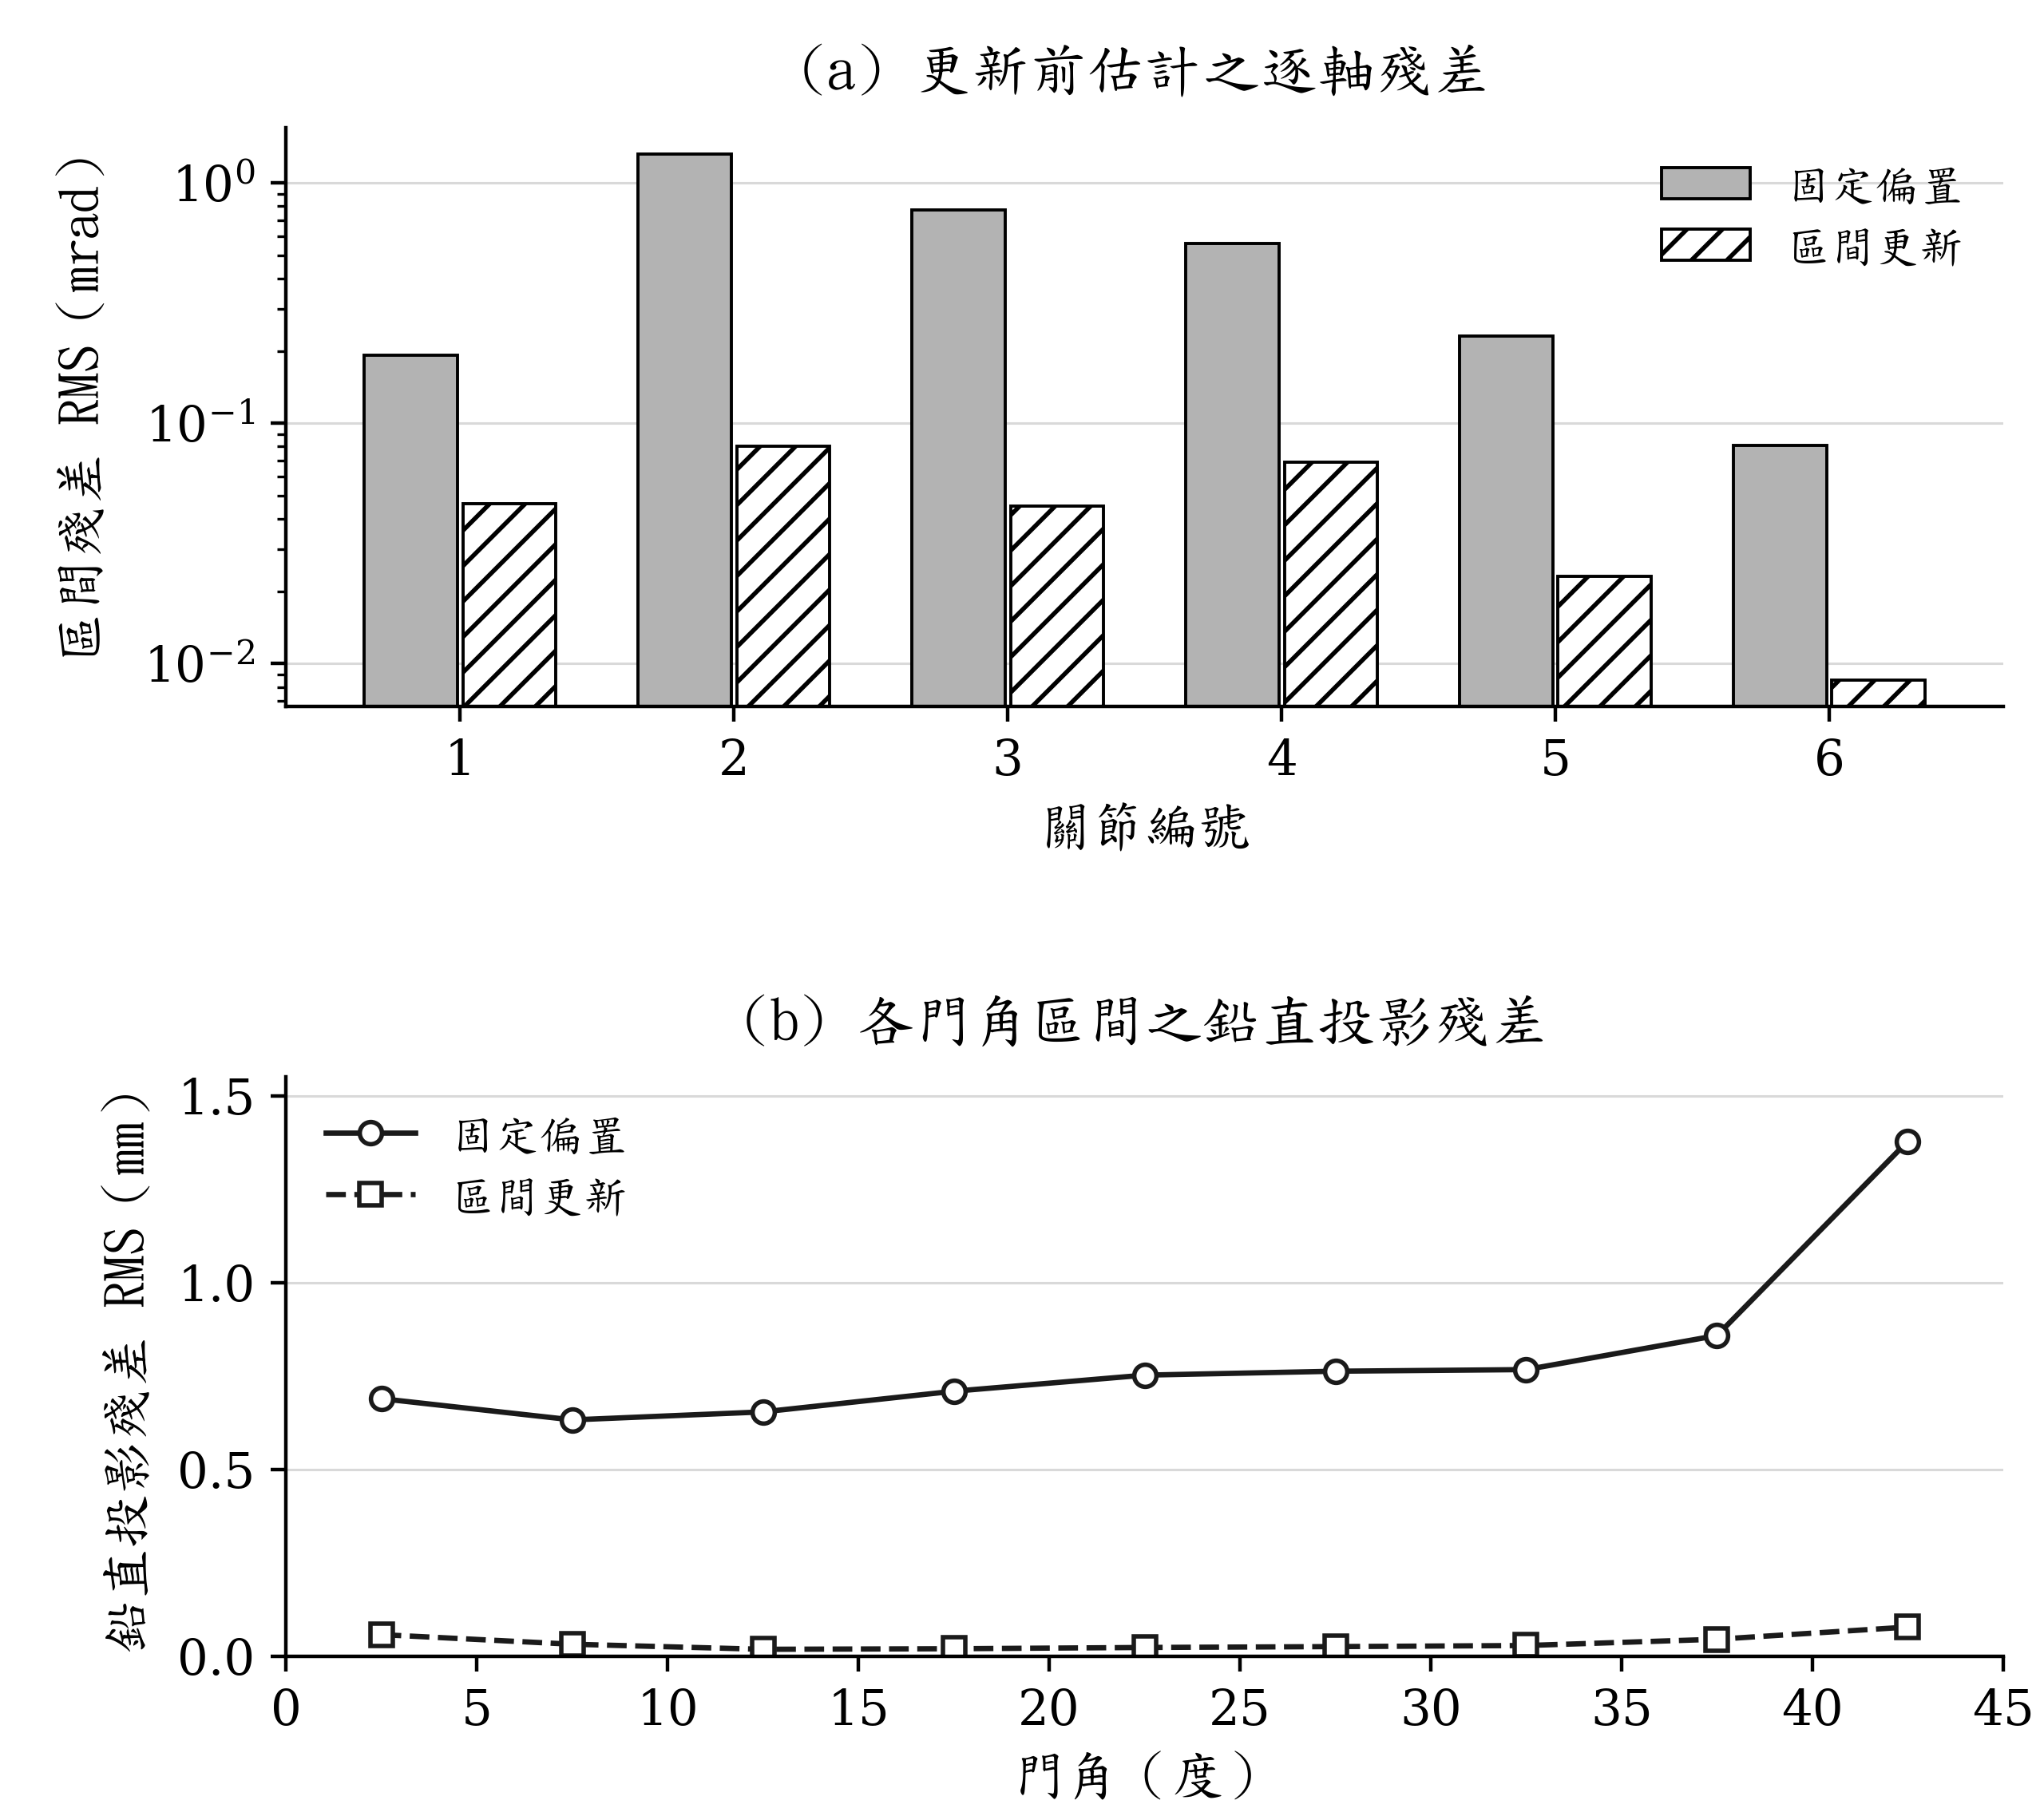
\includegraphics[width=0.98\textwidth]{figsrc/ch04/interval_bias_prediction_residual.png}
    \caption{固定偏置與區間更新之離線重播比較：
    (a) 更新前估計之逐軸區間殘差 RMS，縱軸採對數尺度；
    (b) 依門角每 $5^\circ$ 分組之鉛直投影殘差 RMS，點位於各組角度中點。
    兩條件沿用相同實測軌跡與設定點歷程。}
    \label{fig:ch4_interval_bias_residual}
\end{figure}

偏置重播的結果適用於固定實測軌跡下的區間條件預測。
等效偏移反映位置追蹤模型中的持續差異，
其物理來源可能同時包含構型、負載及未建模動態。
實際控制依任務階段設定偏置的更新與凍結條件，
並以相同參數進行 QP 預測、在途命令前推及停止檢查。
末端積分補償則維持第 3.7 節的有界目標修正方式，
其追蹤效果隨後續操作案例呈現。

% ==================================================
% 4.3 動態導航與避障比較
% ==================================================
\section{動態導航與避障比較}
\label{sec:dynamic_navigation_comparison}

移動機械臂在接近操作區域前，需先通過固定障礙與動態物件交會的空間。
本節以底盤導航控制鏈為評估範圍，
比較本研究導航配置、Nav2 MPPI 與 Regulated Pure Pursuit（RPP）
在相同場景與共同起終點下的到達、淨空及時間表現。
另透過控制屏障函數與原始雷射防護的消融比較，
分析控制求解與命令執行兩個層次對避障結果的影響。
底盤與手臂同時運動的追蹤表現則於第 4.4 節分析。

% ==================================================
% 4.3.1 動態障礙場景與測試配置
% ==================================================
\subsection{動態障礙場景與測試配置}
\label{subsec:dynamic_navigation_scenario_setup}

導航比較於 Gazebo Harmonic 建立的室內場景進行，
場景範圍約為 $20\times20$ m，
配置分隔牆、已知靜態障礙、未加入先驗地圖的靜態障礙，
以及沿設定路段往返的動態物件。
\cref{fig:ch4_dynamic_navigation_scene}呈現平面配置與障礙運動路段。
分隔牆形成不同方向的通行開口，
靜態障礙限制可用空間，
動態物件則在機器人穿越場景時形成交會需求。

\begin{figure}[htbp]
    \centering
    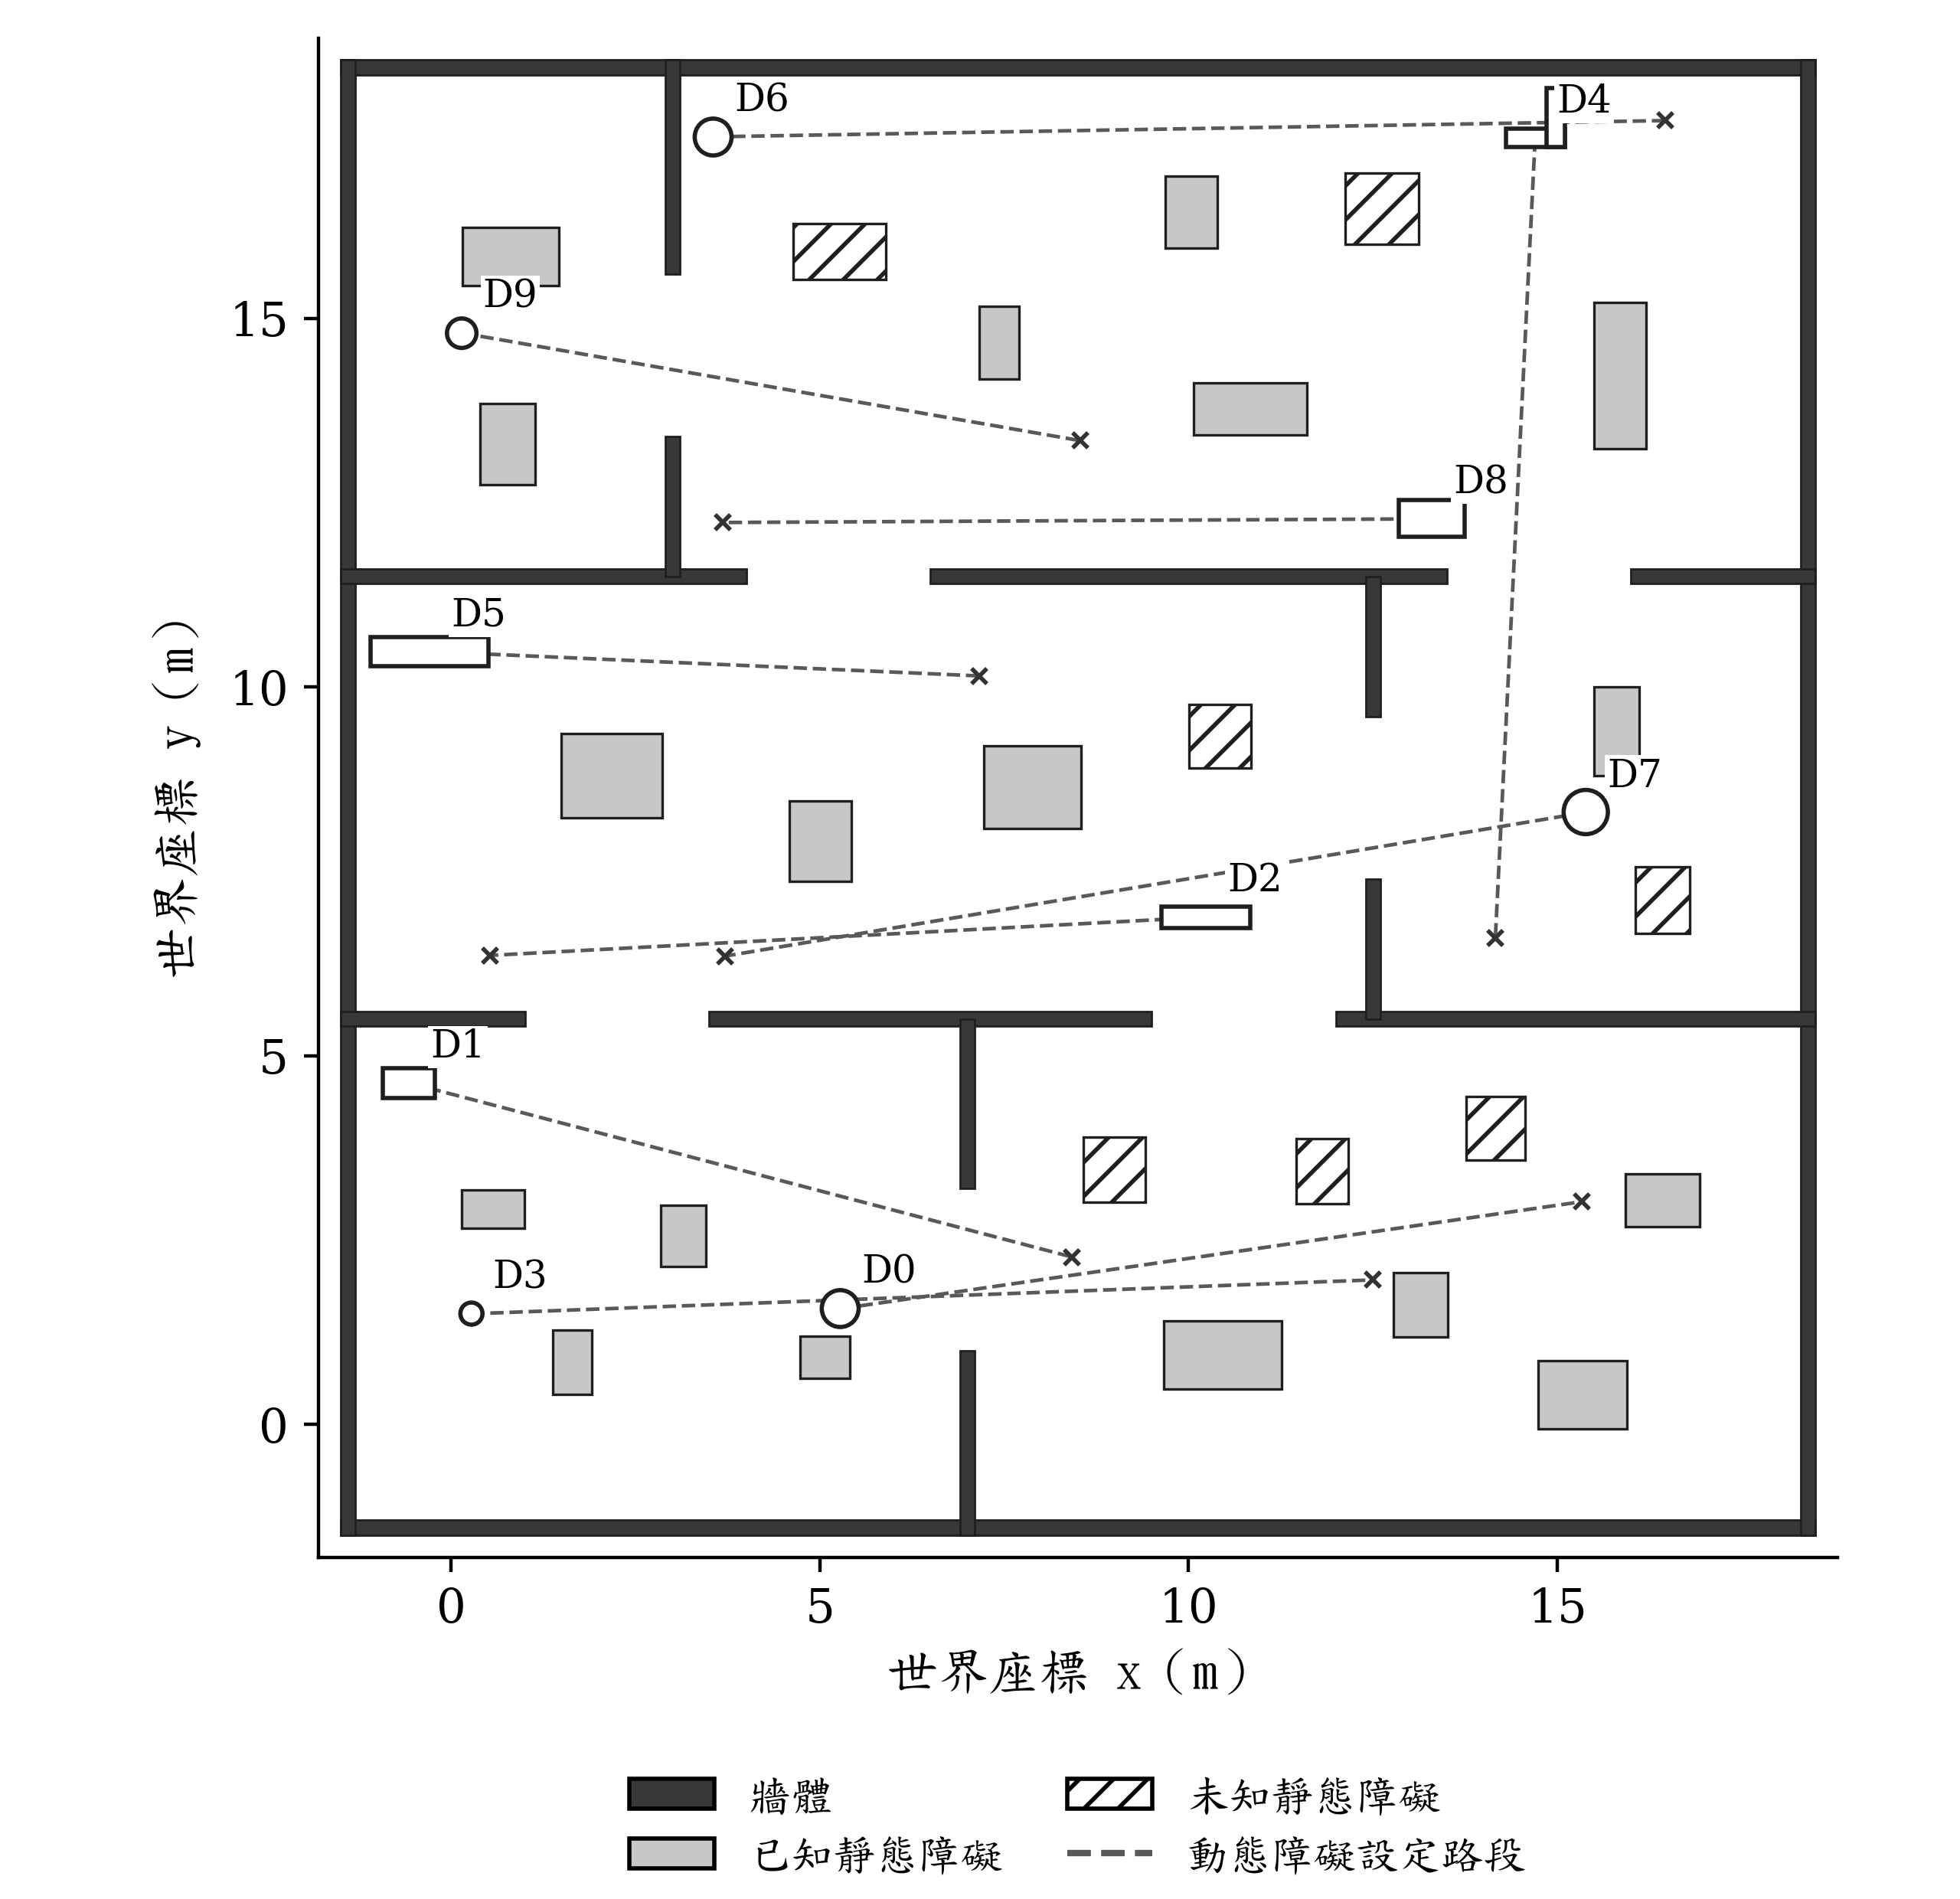
\includegraphics[width=0.92\textwidth]{figsrc/ch04/dynamic_navigation_scene.png}
    \caption{動態導航比較場景之平面配置。
    深色區域為牆體，灰色區域為已知靜態障礙，斜線區域為未知靜態障礙；
    D0--D9 表示動態物件，虛線為設定的往返路段，叉號標示另一端點。}
    \label{fig:ch4_dynamic_navigation_scene}
\end{figure}

動態場景包含十個不同外形的物件，
涵蓋圓柱、矩形與複合外形，設定移動速度介於 $0.10$--$0.14$ m/s。
各方法共用起終點清單、場景幾何及障礙運動設定，
實際交會時機則隨機器人的行進速度與避讓行為改變。
控制器由雷射與各自的感知、代價地圖或追蹤模組取得環境資訊；
模擬器回報的障礙位置另用於離線幾何評估。

本研究導航配置以 SE(2) GMPC 追蹤全域路徑，
於預測時域加入 CBF 限制，
並在命令平滑後以原始雷射防護核對近距離回波。
本組比較固定採用此導航配置，局部側移候選調整關閉。
MPPI 採用 Nav2 的全向運動模型，
以取樣控制序列及軌跡成本更新輸入\cite{nav2mppijazzy}。
RPP 則依路徑前視點與曲率調節前進速度\cite{macenski2023rpp}，
其控制命令包含前進與偏航，側向速度維持為零。

主要條件如\cref{tab:ch4_navigation_settings}所示。
三種方法在可用運動軸上使用相同的執行端速度與命令變化上限，
內部預測時域、取樣方式及成本設定則依各方法配置保留。
MPPI 的內部縱向負加速度界為 $-1.5$ m/s$^2$，
與執行端平滑器的減速限制分別設定。
因此，結果用於比較各導航控制鏈於本全向底盤上的整體表現，
其差異同時包含控制形式與可使用的運動方向。

\begin{table}[htbp]
    \centering
    \caption{動態導航比較之主要設定}
    \label{tab:ch4_navigation_settings}
    \begingroup
    \small
    \renewcommand{\arraystretch}{1.2}
    \begin{tabular}{p{0.31\textwidth} p{0.59\textwidth}}
        \hline
        項目 & 設定 \\
        \hline
        模擬平台與場景 & Gazebo Harmonic，約 $20\times20$ m \\
        動態障礙 & 十個物件，設定速度 $0.10$--$0.14$ m/s \\
        底盤平面外形 & 半徑 $0.30$ m 的圓盤 \\
        控制更新頻率 & $20$ Hz \\
        平移速度上限 & 各可用軸 $0.2775$ m/s；RPP 的 $v_y^B=0$ \\
        偏航速度上限 & $1.1327$ rad/s \\
        執行端命令變化上限
        & 平移 $6.25$ m/s$^2$、偏航 $25.51$ rad/s$^2$ \\
        GMPC 預測時域 & $20$ 步，步長 $0.05$ s，共 $1.0$ s \\
        MPPI 預測與取樣 & $56$ 步，步長 $0.05$ s，共 $2.8$ s；取樣數 $2000$ \\
        到達位置門檻 & 至目標的平面距離小於 $0.30$ m \\
        記錄時間上限 & 牆鐘時間 $250$ s \\
        \hline
    \end{tabular}
    \endgroup
\end{table}

到達結果採用已保存的控制端到達事件與位姿重建判定。
本節到達時間沿用 rosbag 記錄的接收時間戳計算，
與住宅整合任務的模擬時間分別呈現。
淨空統計由首筆全域路徑開始，
至位姿首次進入到達範圍為止；尚未進入時則計算至量測結束。
幾何評估使用底盤與動態物件的模擬位姿，
配合該組資料的靜態距離場及障礙外形近似，
取得每條路線的最小淨空。
複合動態外形於此統計中以主要矩形區塊近似，
幾何重疊結果依此平面評估範圍解讀。

令 $\hat d_r(t)$ 為第 $r$ 條路線在上述評估方式下的淨空，
定義路線最小淨空與幾何重疊指標為
\begin{equation}
    d_{\min,r}=\min_{t\in\mathcal T_r}\hat d_r(t),
    \qquad
    C_r=\mathbb I(d_{\min,r}<0),
    \label{eq:ch4_navigation_overlap_indicator}
\end{equation}
其中 $\mathcal T_r$ 為該路線的評估區間。
當 $C_r=1$ 時，表示評估外形曾出現負淨空。
同一路線內即使重複出現多個負淨空區間，
在重疊路線數中仍只計一次，
以區分路線層級的結果與反覆接近障礙所形成的事件次數。

% ==================================================
% 4.3.2 不同導航方法之性能比較
% ==================================================
\subsection{不同導航方法之性能比較}
\label{subsec:navigation_method_performance}

到達比較採用三種方法皆保有導航結果的 $83$ 條共同路線。
淨空比較另要求三種方法均具有有限且有效的淨空值，
因此使用其中資料完整的 $82$ 條路線；
缺少淨空值的路線仍保留於到達統計。
各方法的到達時間則由其已到達路線計算中位數，
使到達情形、幾何間距與時間各自對應明確的資料集合。

比較結果如\cref{tab:ch4_navigation_method_results}所示。
本研究導航配置完成全部 $83$ 條共同路線，
MPPI 與 RPP 分別到達 $64$ 與 $60$ 條。
在共同淨空集合中，三者的幾何重疊路線數依序為 $1$、$6$ 與 $30$，
每條路線最小淨空的中位數則約為 $0.175$、$0.120$ 與 $0.060$ m。
本研究導航配置在此集合中保留較大的典型間距，
並同時維持較完整的目標到達表現。

\begin{table}[htbp]
    \centering
    \caption{共同路線下之導航方法比較}
    \label{tab:ch4_navigation_method_results}
    \begingroup
    \small
    \setlength{\tabcolsep}{4pt}
    \renewcommand{\arraystretch}{1.25}
    \begin{tabular}{l c c c c}
        \hline
        方法
        & \shortstack{到達路線\\（共 $83$ 條）}
        & \shortstack{重疊路線\\（共 $82$ 條）}
        & \shortstack{最小淨空\\中位數（m）}
        & \shortstack{到達時間\\中位數（s）} \\
        \hline
        本研究導航 & $83$ & $1$  & $0.175$ & $102.6$ \\
        MPPI       & $64$ & $6$  & $0.120$ & $48.6$  \\
        RPP        & $60$ & $30$ & $0.060$ & $73.9$  \\
        \hline
    \end{tabular}
    \endgroup
\end{table}

\cref{fig:ch4_navigation_method_comparison}(a)同時呈現到達與未到達路線，
(b)則以每條路線最小淨空的經驗累積分布比較間距。
對相同淨空門檻，累積比例表示最小淨空不大於該值的路線比例。
本研究導航配置的分布主要位於正淨空區域，
MPPI 與 RPP 則包含較多低淨空或負淨空路線。
其中本研究導航配置的最差估計淨空約為 $-0.0012$ m，
對應一次接近幾何邊界的輕微重疊。

\begin{figure}[htbp]
    \centering
    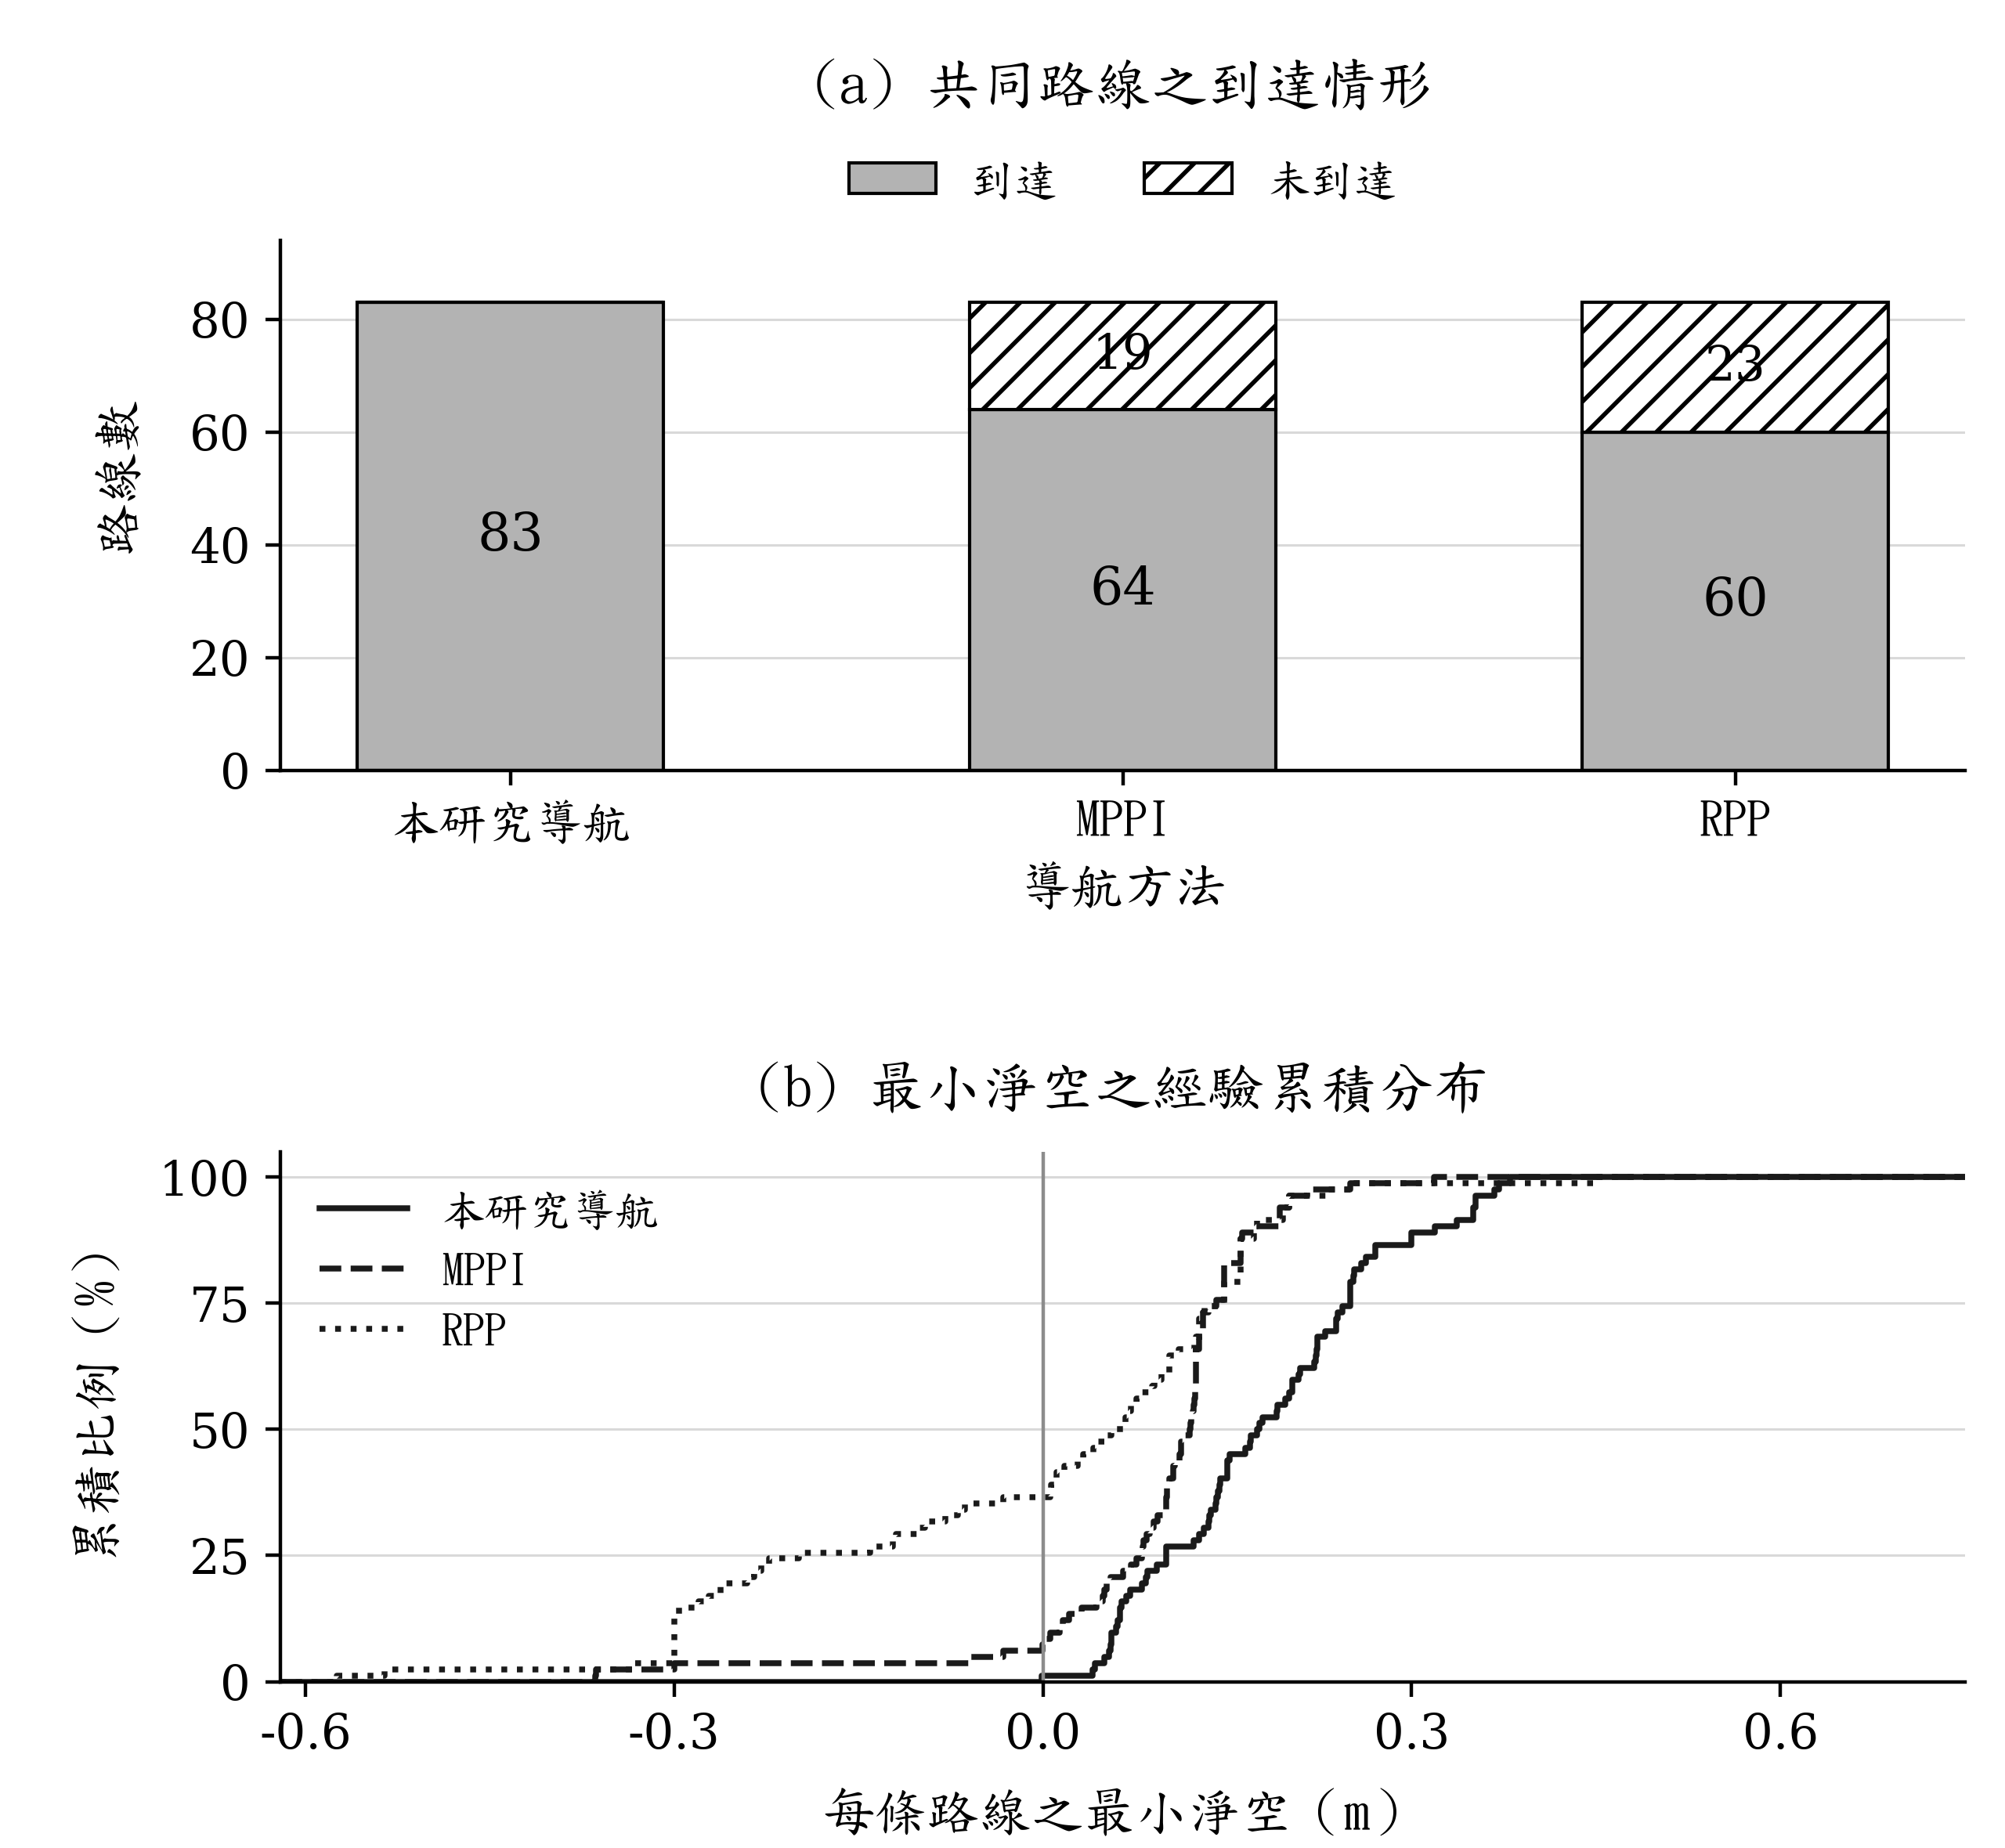
\includegraphics[width=0.98\textwidth]{figsrc/ch04/navigation_method_comparison.png}
    \caption{不同導航方法之到達與淨空比較：
    (a) $83$ 條共同路線的到達情形；
    (b) $82$ 條共同有效路線之最小淨空經驗累積分布。
    (b) 中零淨空左側對應評估外形曾出現幾何重疊的路線。}
    \label{fig:ch4_navigation_method_comparison}
\end{figure}

三者的到達時間中位數分別為 $102.6$、$48.6$ 與 $73.9$ s。
本研究導航配置需要較長時間完成通行，
其到達完整性與間距表現伴隨較高的時間成本。
由於各方法成功到達的路線集合不同，
時間中位數需與到達數量共同解讀；
較短時間可能同時反映較快行進與較困難路線未完成的選樣差異。

本研究導航配置將障礙相對運動納入 CBF，
並以原始掃描限制近距離接近速度；
MPPI 則依其取樣軌跡與代價地圖評分更新命令，
RPP 依前視路徑調整前進與轉向。
上述結果反映這些完整配置在本場景中的行為差異，
可用運動方向、預測時域與避障處理方式均屬比較條件的一部分。

% ==================================================
% 4.3.3 控制屏障與雷射防護之消融比較
% ==================================================
\subsection{控制屏障與雷射防護之消融比較}
\label{subsec:cbf_scan_shield_ablation}

為分析兩個避障層次的作用，
以相同 GMPC 路徑追蹤控制器建立四種配置：
A 為兩者皆關閉，B 僅啟用 CBF，
C 僅啟用原始雷射防護，D 則同時啟用兩者。
比較使用四種配置皆具有效結果的 $28$ 條共同路線，
並保留相同場景、起終點、速度上限與其餘控制設定。
四種配置在此集合中皆到達目標，
因此可在相同到達範圍下比較幾何重疊與時間成本。

\cref{tab:ch4_navigation_ablation}列出消融結果。
配置 A 的幾何重疊路線數為 $22$；
加入 CBF 後，配置 B 降至 $3$，
僅啟用雷射防護的配置 C 則為 $2$。
配置 D 在本次共同集合中未記錄到負淨空，
且全部路線中的最差淨空約為 $0.022$ m。
這些結果顯示，兩種模組各自啟用時均能減少幾何重疊，
共同啟用時則在本集合中取得較完整的通行結果。

\begin{table}[htbp]
    \centering
    \caption{CBF 與原始雷射防護之消融比較（共同 $28$ 條路線）}
    \label{tab:ch4_navigation_ablation}
    \begingroup
    \small
    \setlength{\tabcolsep}{4pt}
    \renewcommand{\arraystretch}{1.25}
    \begin{tabular}{c c c c c c}
        \hline
        配置 & CBF & 雷射防護
        & \shortstack{重疊\\路線數}
        & \shortstack{最小淨空\\中位數（m）}
        & \shortstack{到達時間\\中位數（s）} \\
        \hline
        A & 關 & 關 & $22$ & $-0.300$ & $79.2$  \\
        B & 開 & 關 & $3$  & $0.180$  & $98.0$  \\
        C & 關 & 開 & $2$  & $0.080$  & $88.4$  \\
        D & 開 & 開 & $0$  & $0.150$  & $104.3$ \\
        \hline
    \end{tabular}
    \endgroup
\end{table}

兩個模組作用於不同的資料與命令位置。
CBF 由追蹤後的障礙幾何與速度建立預測限制，
使避障需求直接參與控制輸入的求解；
原始雷射防護則在執行端處理有效回波，
限制最終命令沿近距離障礙方向的接近分量。
因此，兩者分別提供預測限制與執行端命令核對，
其組合效果可由 B、C 與 D 的差異觀察。

\cref{fig:ch4_navigation_ablation}(a)比較幾何重疊路線數，
(b)呈現相同路線集合下的到達時間分布。
配置 D 的時間中位數為 $104.3$ s，
高於配置 B 的 $98.0$ s 與配置 C 的 $88.4$ s。
其路徑長度中位數亦由配置 A 的約 $19.0$ m 增至 $21.8$ m，
反映此避障配置下較高的通行時間與路程成本。

\begin{figure}[htbp]
    \centering
    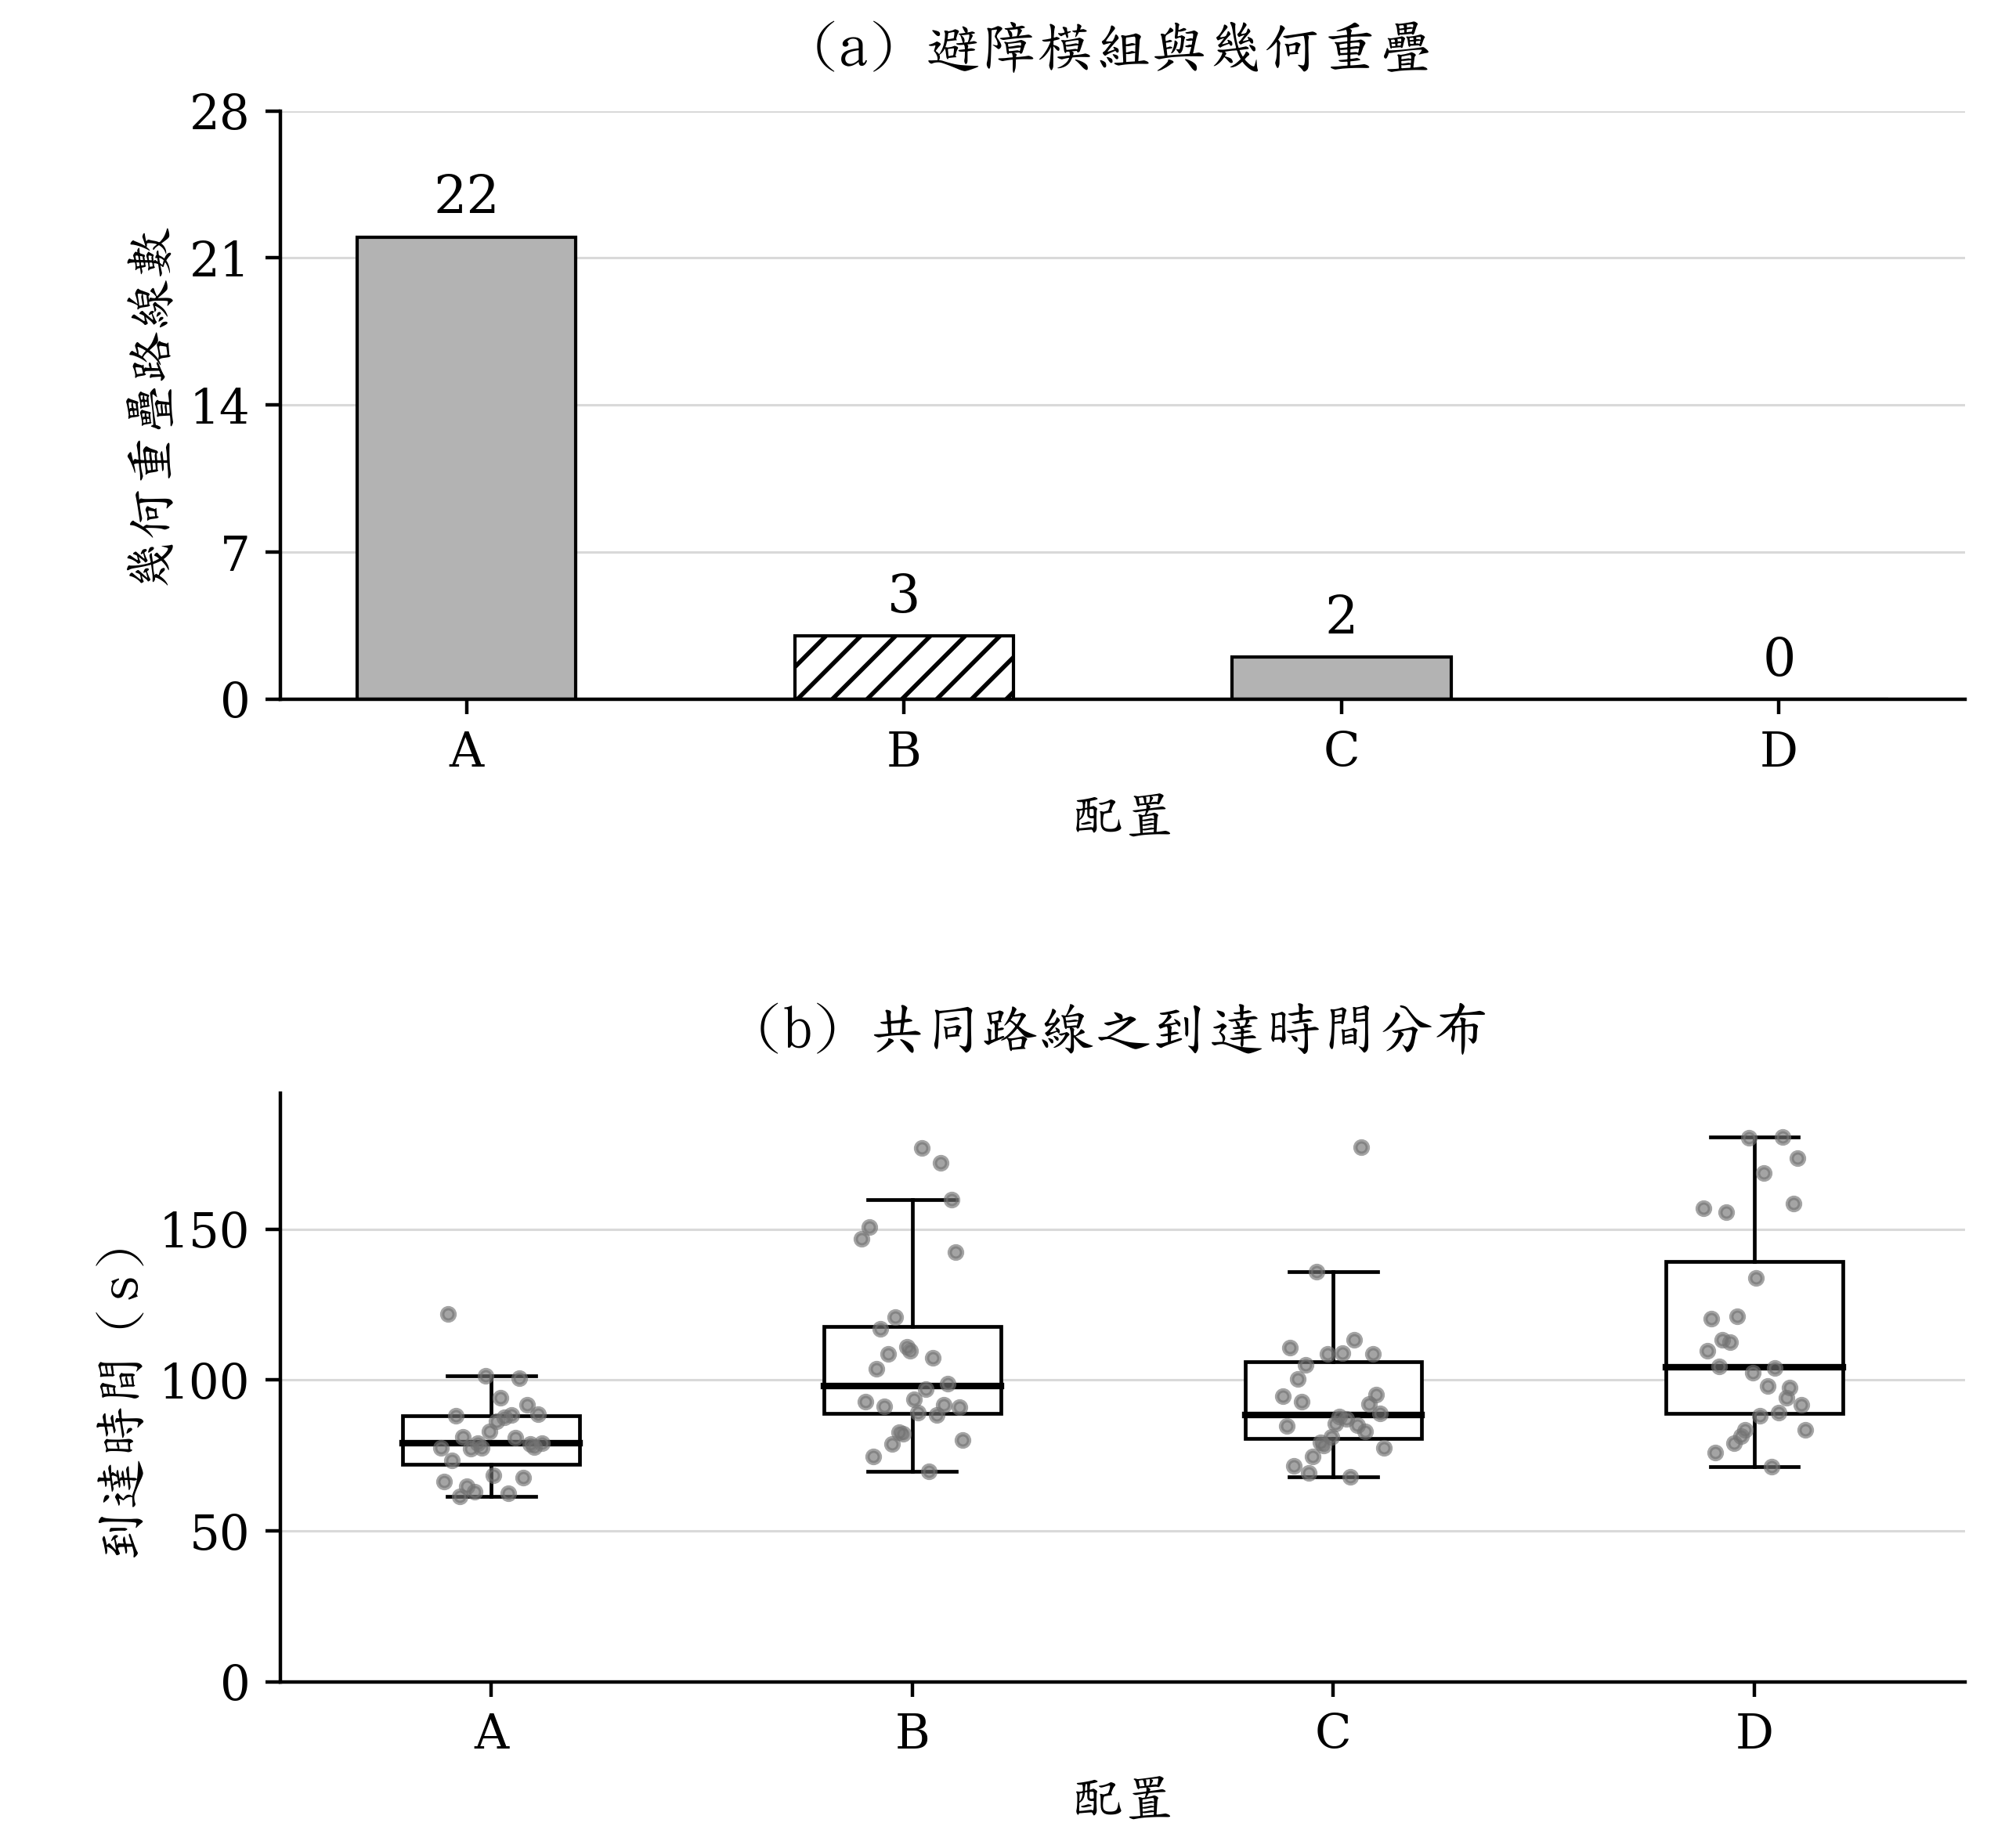
\includegraphics[width=0.98\textwidth]{figsrc/ch04/cbf_scan_shield_ablation.png}
    \caption{避障模組消融比較：
    (a) 共同路線中出現幾何重疊的路線數；
    (b) 到達時間分布，散點為各路線結果，箱體為第 $25$ 至 $75$ 百分位數，
    中線為中位數，鬚線為 $1.5$ 倍四分位距內的資料範圍。
    A 為兩者關閉，B 僅啟用 CBF，C 僅啟用雷射防護，D 為兩者啟用。}
    \label{fig:ch4_navigation_ablation}
\end{figure}

配置 B 的典型最小淨空高於配置 D，
但仍保有負淨空路線，說明單一中位數無法涵蓋全部交會情形。
同時檢查到達、重疊路線、最差淨空與時間分布，
可較完整地呈現避障配置的效果與代價。
本組結果支持在所測場景與速度範圍下保留兩層防護，
並於後續全身操作中持續核對其命令作用與任務銜接。

% ==================================================
% 4.4 全身協同操作與預測時域比較
% ==================================================
\section{全身協同操作與預測時域比較}
\label{sec:wholebody_horizon_comparison}

全身控制需在底盤移動的同時維持末端追蹤，
並使手臂設定點的累積與關節響應符合物件操作需求。
本節以獨立抽屜場景分析底盤與手臂的運動分工，
再比較單步與五步控制的追蹤、命令變化及計算成本，
最後以完整開關抽屜與返回任務，比較移動中操作與停駐後操作的時間。
各組資料沿用取得時的控制與接觸設定；
本節操作目標由場景幾何建立，住宅場景的視覺導引與任務整合於第 4.5 節說明。

% ==================================================
% 4.4.1 底盤與末端協同追蹤表現
% ==================================================
\subsection{底盤與末端協同追蹤表現}
\label{subsec:base_tcp_coordinated_tracking}

抽屜場景使用具有單一滑動自由度的被動機構，
把手橫桿直徑為 $26$ mm，目標開度為 $200$ mm。
控制週期為 $0.05$ s，物理步長為 $0.01$ s，
手臂仍以設定點變化率作為輸入。
任務依序執行接近、夾持、拉開、開啟保持、推回、關閉保持與退出，
再收臂並返回起點。
開啟與關閉分別要求在 $195$--$205$ mm 與 $0$--$5$ mm 的範圍連續保持至少 $2$ s；
夾持建立則要求雙指接觸力皆達 $0.5$ N 並連續維持至少 $2$ s。
底盤配合滑軌方向移動，手臂同步調整構型以追蹤把手位姿。

為呈現兩者的幾何分工，令
$f(b,q_a)$ 表示由底盤位姿與手臂構型計算的 TCP 世界位置，
$b_0,q_{a,0}$ 為拉開開始時的構型，
$a_d$ 為滑軌開啟方向的單位向量。
依序代入底盤與手臂構型，定義軸向位移分量：
\begin{equation}
    \begin{aligned}
        \Delta\ell_B(t)
        &=a_d^\top\!\left[f(b(t),q_{a,0})-f(b_0,q_{a,0})\right],\\
        \Delta\ell_A(t)
        &=a_d^\top\!\left[f(b(t),q_a(t))-f(b(t),q_{a,0})\right],\\
        \Delta\ell_E(t)&=\Delta\ell_B(t)+\Delta\ell_A(t).
    \end{aligned}
    \label{eq:ch4_coordinated_displacement_decomposition}
\end{equation}
底盤分量包含平移與偏航對 TCP 的共同作用，
手臂分量則在當時底盤位姿下計算。
此分解為構型變化的幾何描述，其數值依上述代入順序定義。

以時域比較中配對案例一的五步控制紀錄為例，
\cref{fig:ch4_wholebody_drawer_coordination}(a)顯示拉開至推回期間的位移。
開始開啟保持時，TCP 沿滑軌方向累積移動約 $195.2$ mm，
其中底盤與手臂幾何分量分別約為 $139.6$ 與 $55.7$ mm。
推回時，兩者共同減少末端的軸向位移，
使 TCP 隨把手返回關閉位置。
這項結果呈現底盤對操作位移的實際參與，
手臂同時承接末端追蹤所需的剩餘構型變化。

\begin{figure}[htbp]
    \centering
    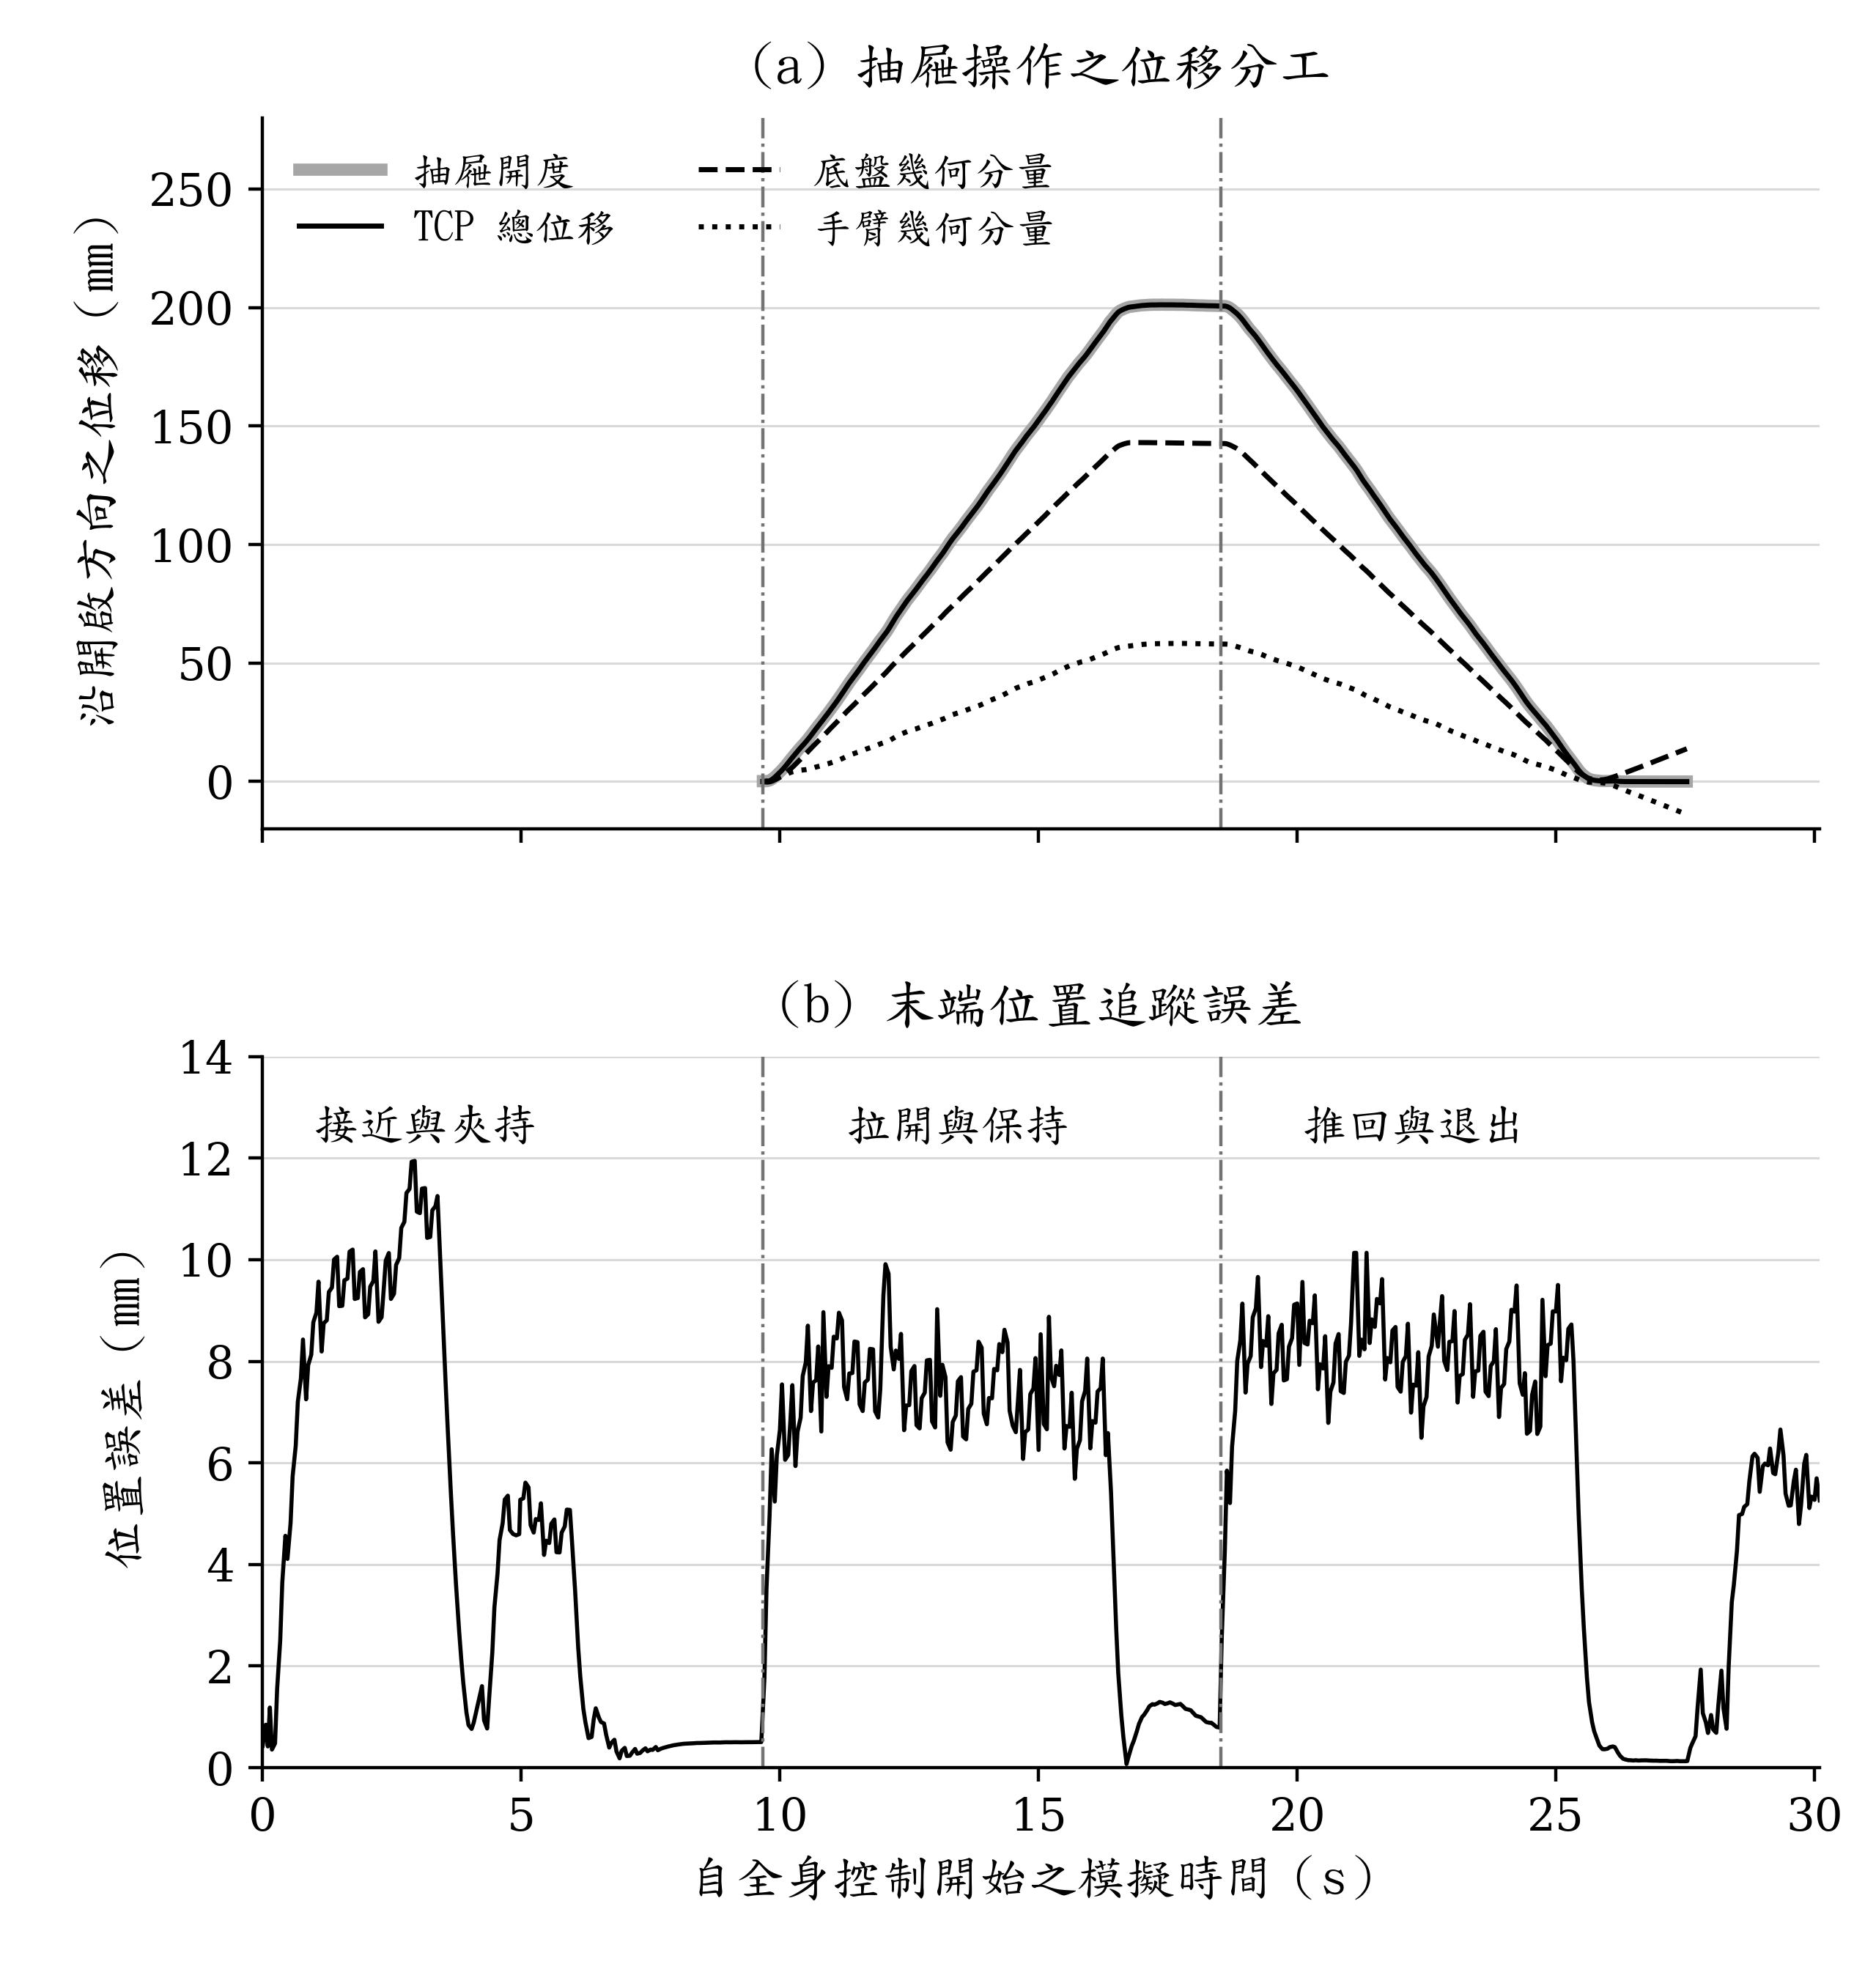
\includegraphics[width=0.98\textwidth]{figsrc/ch04/wholebody_drawer_coordination.png}
    \caption{配對案例一之五步全身控制結果：
    (a) 抽屜開度、TCP 軸向總位移與底盤及手臂幾何分量，位移以拉開起點為基準；
    (b) 全身控制區間之末端位置追蹤誤差。
    點畫直線分別標示拉開與推回開始時刻。}
    \label{fig:ch4_wholebody_drawer_coordination}
\end{figure}

\cref{fig:ch4_wholebody_drawer_coordination}(b)呈現同一案例的末端位置誤差。
接近、拉開與推回期間的誤差高於定點保持階段，
因此整段追蹤統計需配合任務階段解讀。
三個五步控制案例的位置誤差第 $95$ 百分位數為 $7.27$--$9.75$ mm，
姿態誤差第 $95$ 百分位數為 $0.207$--$0.300^\circ$。
實際關節位置與設定點至有效限位的最小餘量，
分別約為 $0.785$--$0.795$ rad 與 $0.783$--$0.793$ rad，
顯示此組運動仍保留關節範圍。
以下進一步比較相同任務下，預測步數改變所伴隨的追蹤與命令差異。

% ==================================================
% 4.4.2 單步與多步控制之比較
% ==================================================
\subsection{單步與多步控制之比較}
\label{subsec:single_multistep_control_comparison}

時域比較使用同一設定點增廣控制模型，
分別設定 $N=1$ 與 $N=5$，對應 $50$ 與 $250$ ms 的預測長度。
兩組共用任務流程、追蹤權重、命令限制與執行補償設定，
並以三組配對案例比較。
預測期間重複使用當輪取得的末端目標與協同參考，
未提供未來操作目標序列。
主要設定如\cref{tab:ch4_horizon_control_settings}所示。

\begin{table}[htbp]
    \centering
    \caption{單步與五步控制之比較設定}
    \label{tab:ch4_horizon_control_settings}
    \begingroup
    \small
    \renewcommand{\arraystretch}{1.2}
    \begin{tabular}{p{0.38\textwidth} c c}
        \hline
        項目 & 單步控制 & 五步控制 \\
        \hline
        預測步數 $N$ & $1$ & $5$ \\
        控制步長 & $0.05$ s & $0.05$ s \\
        預測時間長度 & $0.05$ s & $0.25$ s \\
        控制序列變數數量 $9N$ & $9$ & $45$ \\
        終端任務追蹤倍率 & $5$ & $5$ \\
        輸入與協同成本累加步數 & $1$ & $5$ \\
        時域內目標 & 當輪目標固定 & 當輪目標固定 \\
        配對案例數 & $3$ & $3$ \\
        \hline
    \end{tabular}
    \endgroup
\end{table}

終端倍率相同仍會隨預測步數改變成本結構。
令 $\ell_{T,i}$ 為第 $i$ 步受終端倍率作用的任務追蹤成本，
$\ell_{O,i}$ 為同一步對應的其餘輸入、命令變化與協同成本，
則兩組累加形式為
\begin{equation}
    \begin{aligned}
        J_{N=1}&=5\ell_{T,1}+\ell_{O,1},\\
        J_{N=5}&=\sum_{i=1}^{4}\ell_{T,i}
                   +5\ell_{T,5}+\sum_{i=1}^{5}\ell_{O,i}.
    \end{aligned}
    \label{eq:ch4_horizon_cost_accumulation}
\end{equation}
單步的唯一追蹤項即為放大的終端項，
五步則同時包含前四步追蹤與五份其餘成本。
因此，本組結果反映預測長度、終端項位置及成本累加比例共同形成的控制表現。

追蹤與命令統計的評估區間由首輪全身求解開始，
至退出完成且求解節點停止為止，
不包含進場導航、前段展臂、後續收臂與返回。
命令增量採相鄰求解輪送出的六軸手臂命令，
每次取各軸絕對差的最大值，再統計第 $95$ 百分位數。
其單位仍為 rad/s，表示設定點變化率的差異。
命令反轉則逐軸計算同一階段內，
相鄰兩輪絕對值皆大於 $0.05$ rad/s 且符號相反的次數，
再以整段控制時間換算反轉率。

六個案例皆完成任務並通過既定操作判準。
\cref{tab:ch4_horizon_control_results}列出三個案例各自統計值的範圍，
\cref{fig:ch4_horizon_tracking_comparison}則保留同一案例的配對關係。
五步控制的位置誤差第 $95$ 百分位數為 $7.27$--$9.75$ mm，
低於單步控制的 $10.78$--$16.64$ mm；
姿態誤差亦由單步的 $0.410$--$0.484^\circ$，
降至五步的 $0.207$--$0.300^\circ$。
手臂命令增量與反轉率在三組配對中皆較低，
表示五步配置在此任務中同時減少整段追蹤偏差與週期間命令反轉。

\begin{table}[htbp]
    \centering
    \caption{單步與五步控制結果之案例範圍（各三個案例）}
    \label{tab:ch4_horizon_control_results}
    \begingroup
    \small
    \setlength{\tabcolsep}{4pt}
    \renewcommand{\arraystretch}{1.25}
    \begin{tabular}{p{0.45\textwidth} c c}
        \hline
        指標 & 單步控制 & 五步控制 \\
        \hline
        位置誤差第 $95$ 百分位數（mm） & $10.78$--$16.64$ & $7.27$--$9.75$ \\
        姿態誤差第 $95$ 百分位數（度） & $0.410$--$0.484$ & $0.207$--$0.300$ \\
        手臂命令增量第 $95$ 百分位數（rad/s） & $0.340$--$0.360$ & $0.145$--$0.193$ \\
        手臂命令反轉率（次/s） & $26.01$--$28.42$ & $1.12$--$2.33$ \\
        夾持期間最大相對位移（mm） & $2.392$--$3.805$ & $0.104$--$0.388$ \\
        全身控制區間（s） & $37.41$--$59.43$ & $30.10$--$35.58$ \\
        核心計算耗時中位數（ms） & $6.4$--$9.0$ & $17.9$--$21.7$ \\
        \hline
    \end{tabular}
    \endgroup
\end{table}

\begin{figure}[htbp]
    \centering
    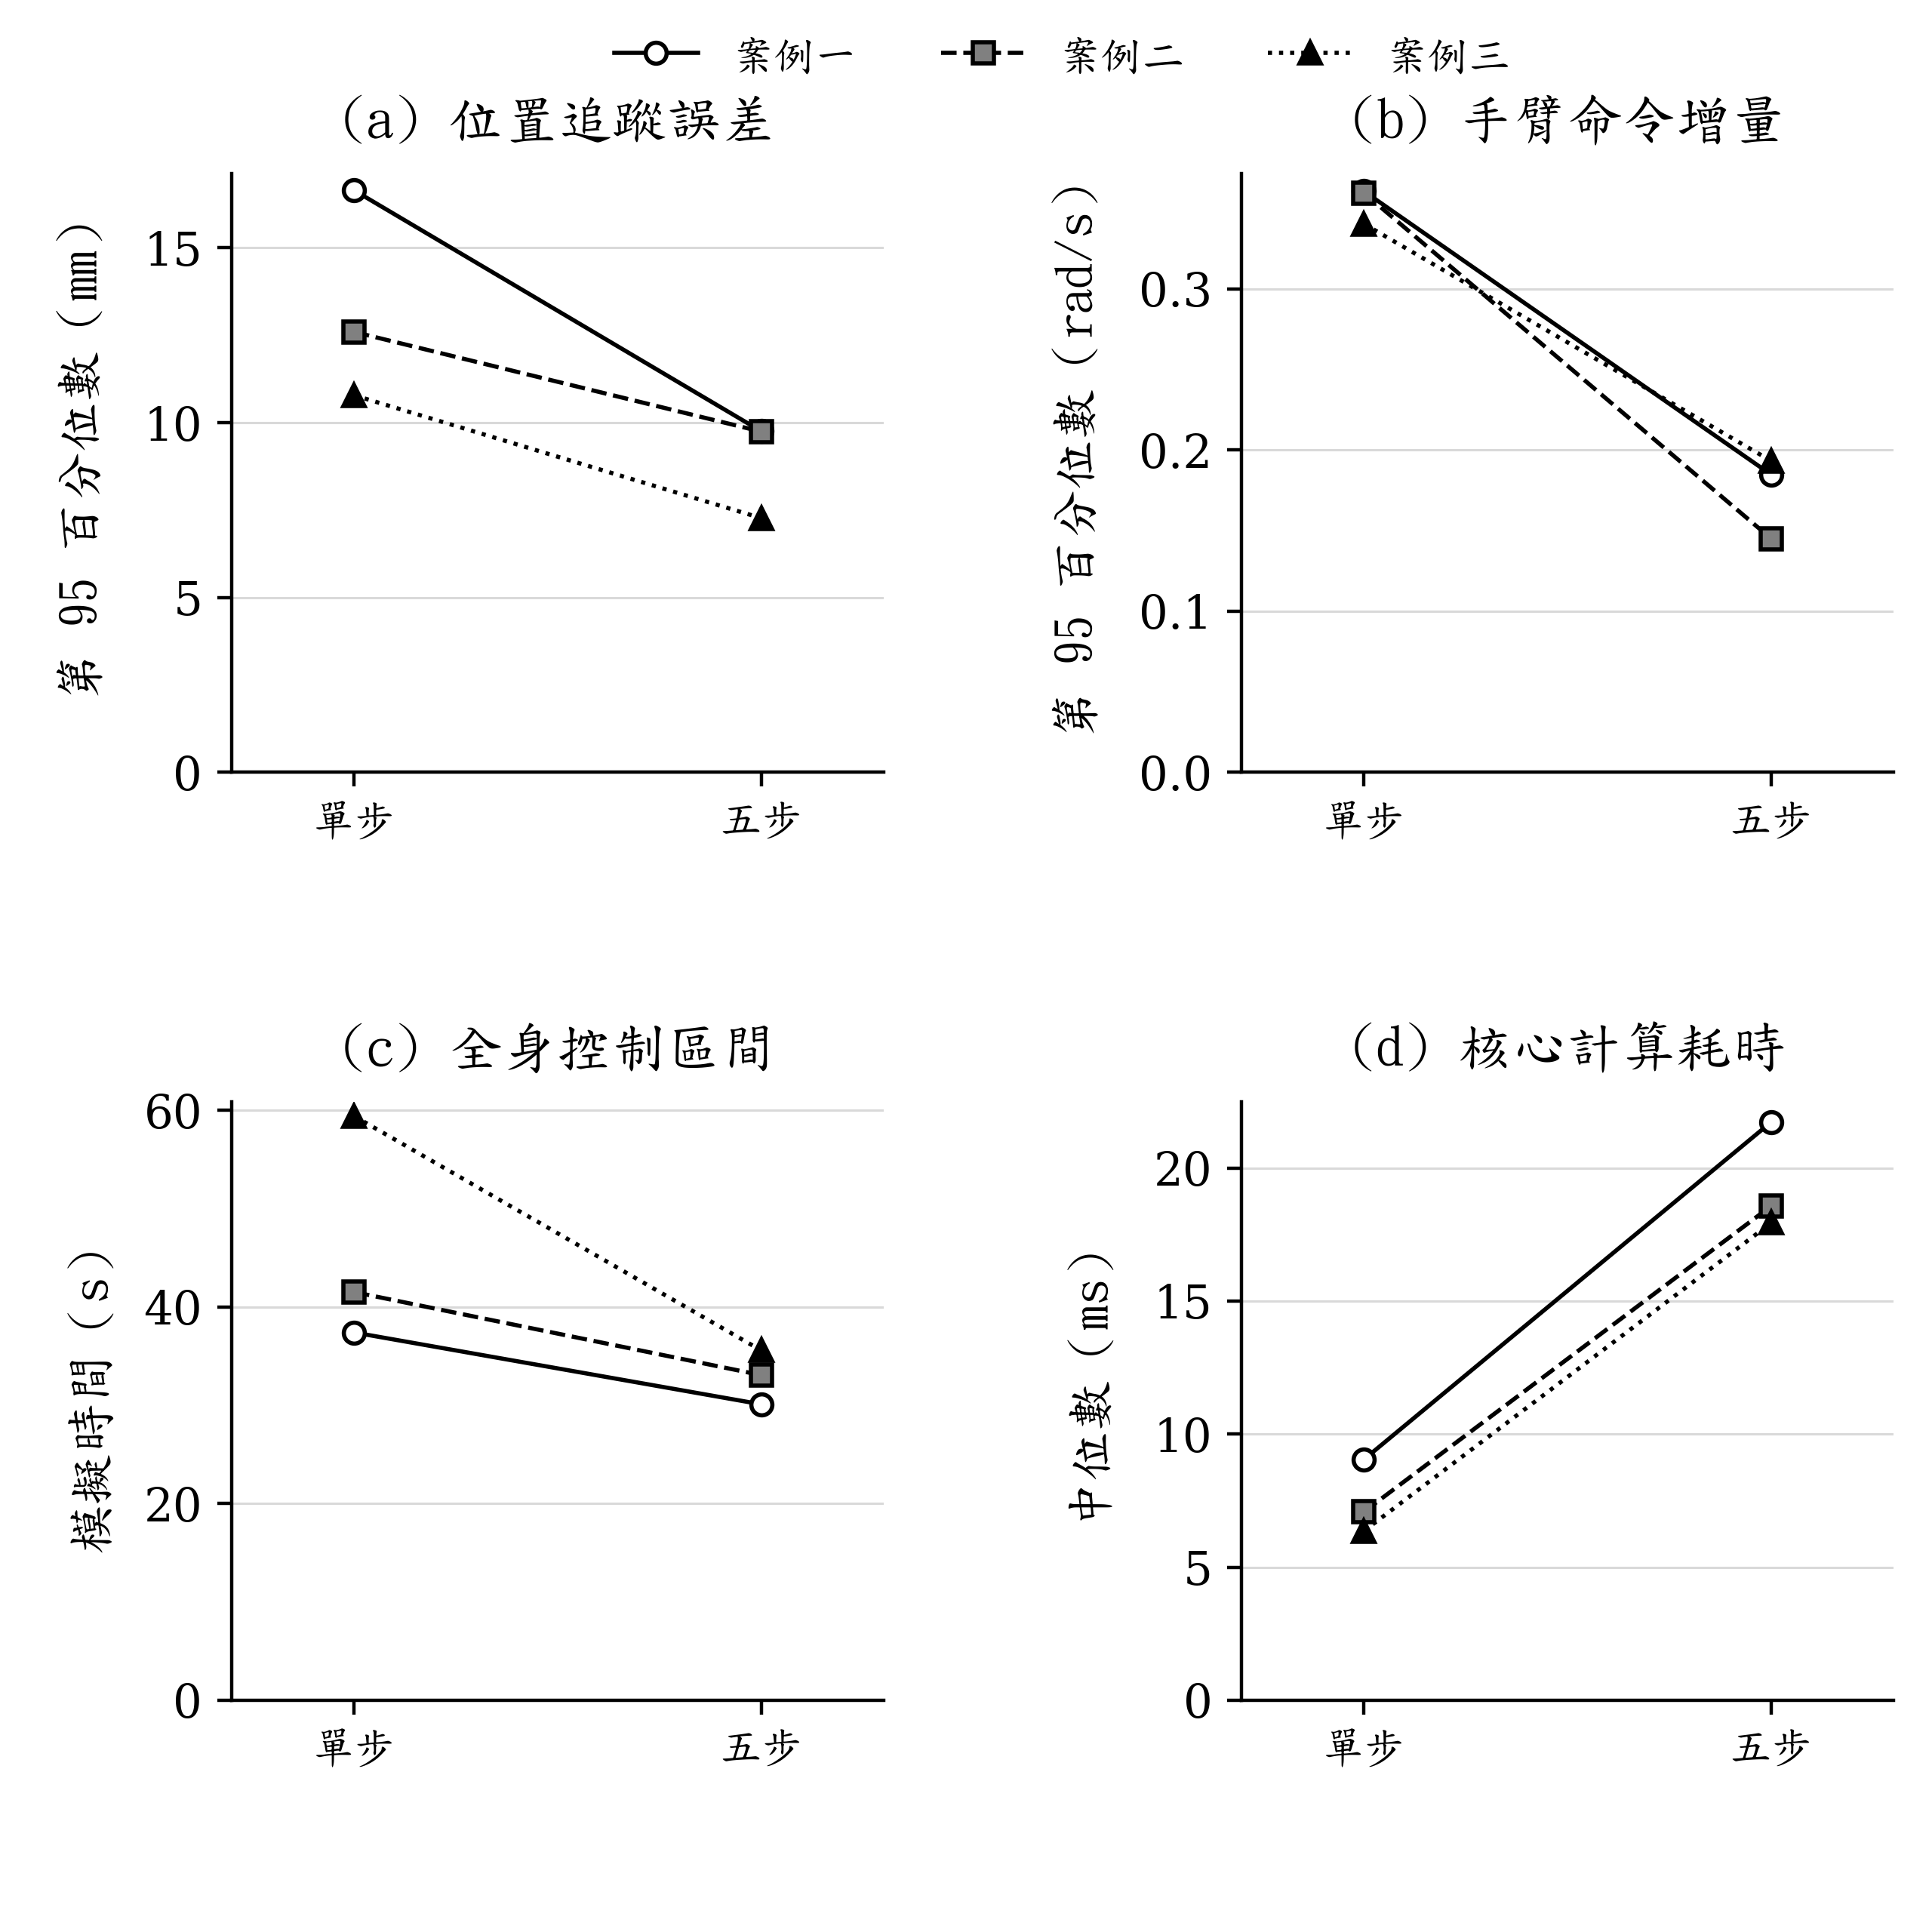
\includegraphics[width=0.98\textwidth]{figsrc/ch04/horizon_tracking_comparison.png}
    \caption{單步與五步控制之配對比較：
    (a) 位置誤差第 $95$ 百分位數；
    (b) 手臂命令增量第 $95$ 百分位數；
    (c) 全身控制區間；(d) 核心計算耗時中位數。
    各線連接同一配對案例；(c) 使用模擬時間，(d) 使用主機時間。}
    \label{fig:ch4_horizon_tracking_comparison}
\end{figure}

五步控制的控制區間分別為 $30.10$、$33.07$ 與 $35.58$ s，
相對應的單步配置則為 $37.41$、$41.52$ 與 $59.43$ s，
配對差介於 $7.31$--$23.85$ s。
五步配置的核心計算耗時中位數較高，
呈現單次計算成本與任務推進時間之間的取捨。
此處計算耗時包含當時求解流程的局部近似與最佳化運算，
各組的執行順序與主機熱狀態仍有差異，
其耗時差值須連同執行條件解讀。

整段統計的改善亦有階段差異。
例如配對案例二在開啟保持階段，
單步與五步的位置誤差第 $95$ 百分位數分別約為 $0.91$ 與 $1.47$ mm，
該階段由單步配置取得較低誤差。
本組三對資料據此支持五步配置在整段追蹤、命令變化與控制區間上的改善，
其適用範圍仍限於上述抽屜任務、成本與控制設定。

% ==================================================
% 4.4.3 抽屜操作之移動與停駐策略比較
% ==================================================
\subsection{抽屜操作之移動與停駐策略比較}
\label{subsec:moving_parked_drawer_strategy}

操作策略比較另採用三組配對資料，兩組皆使用五步全身控制。
移動中操作允許底盤在接近與開關抽屜期間配合手臂移動；
停駐後操作則先完成底盤減速與定位，再以位置保持伺服維持底盤，
由手臂完成接近、拉開與推回。
兩組共用抽屜、起終點、開關保持條件及當時的偏置觀測設定，
並交替安排執行順序。
停駐組另固定預測期間的底盤輸入並停用近目標命令整形，
因此本項比較涵蓋進場、接手與運動安排等完整策略的差異。

完整任務時間以模擬時鐘計算，
由首次發布導航計畫起算，至開啟與關閉保持條件皆完成、
控制權已交還導航，且底盤首次返回起點 $0.20$ m 範圍內為止。
任務完成時間由逐物理步狀態獨立判定，
並與任務結束事件交叉核對，兩者差異皆不超過 $0.04$ s。
此時間涵蓋進場、接近、開關、退出、收臂與返回，
與前節僅涵蓋全身控制的評估區間分別計算。

停駐條件亦在實際接手至交還導航的完整區間內核對。
三個停駐案例的最大底盤平移速度為 $0.930$--$0.975$ mm/s，
相對停駐錨點的最大位置偏差為 $0.479$--$0.487$ mm，
最大朝向偏差為 $0.207$--$0.250^\circ$，
皆符合所設定的 $1$ mm/s、$1$ mm 與 $0.5^\circ$ 上限。
此核對使停駐策略的結果能對應至實際底盤保持狀態。

\cref{tab:ch4_moving_parked_drawer_results}列出完整任務時間。
六個案例皆完成開關抽屜與返回，
移動策略的平均時間為 $80.72$ s，停駐策略為 $93.62$ s。
三組配對皆由移動策略取得較短時間，
縮短量為 $12.51$--$13.19$ s，
依式\eqref{eq:ch4_task_time_comparison}計算的時間縮短比例為 $13.38$--$14.05\%$。

\begin{table}[htbp]
    \centering
    \caption{移動中操作與停駐後操作之完整任務時間比較}
    \label{tab:ch4_moving_parked_drawer_results}
    \begingroup
    \small
    \setlength{\tabcolsep}{5pt}
    \renewcommand{\arraystretch}{1.25}
    \begin{tabular}{c c c c c}
        \hline
        配對案例
        & \shortstack{移動中操作\\（s）}
        & \shortstack{停駐後操作\\（s）}
        & \shortstack{時間縮短\\（s）}
        & \shortstack{縮短比例\\（\%）} \\
        \hline
        一 & $80.99$ & $93.50$ & $12.51$ & $13.38$ \\
        二 & $80.70$ & $93.89$ & $13.19$ & $14.05$ \\
        三 & $80.46$ & $93.48$ & $13.02$ & $13.93$ \\
        \hline
    \end{tabular}
    \endgroup
\end{table}

\cref{fig:ch4_moving_parked_drawer_comparison}(b)將時間差依任務事件分段。
由出發至全身接手的平均時間差約為 $11.40$ s，
包含進場減速、位置與朝向收斂及不同接手條件。
停駐組的靜止觀察區間約為 $0.51$ s，
僅占上述差距的一部分。
全身接手至夾持成立期間，移動策略平均多用約 $1.90$ s；
若改由共同出發事件計算至夾持成立，
移動策略仍較快 $9.09$--$9.76$ s。
因此，較早接手帶來的時間收益，
需與接手後仍持續進行的接近及穩定過程一併評估。

\begin{figure}[htbp]
    \centering
    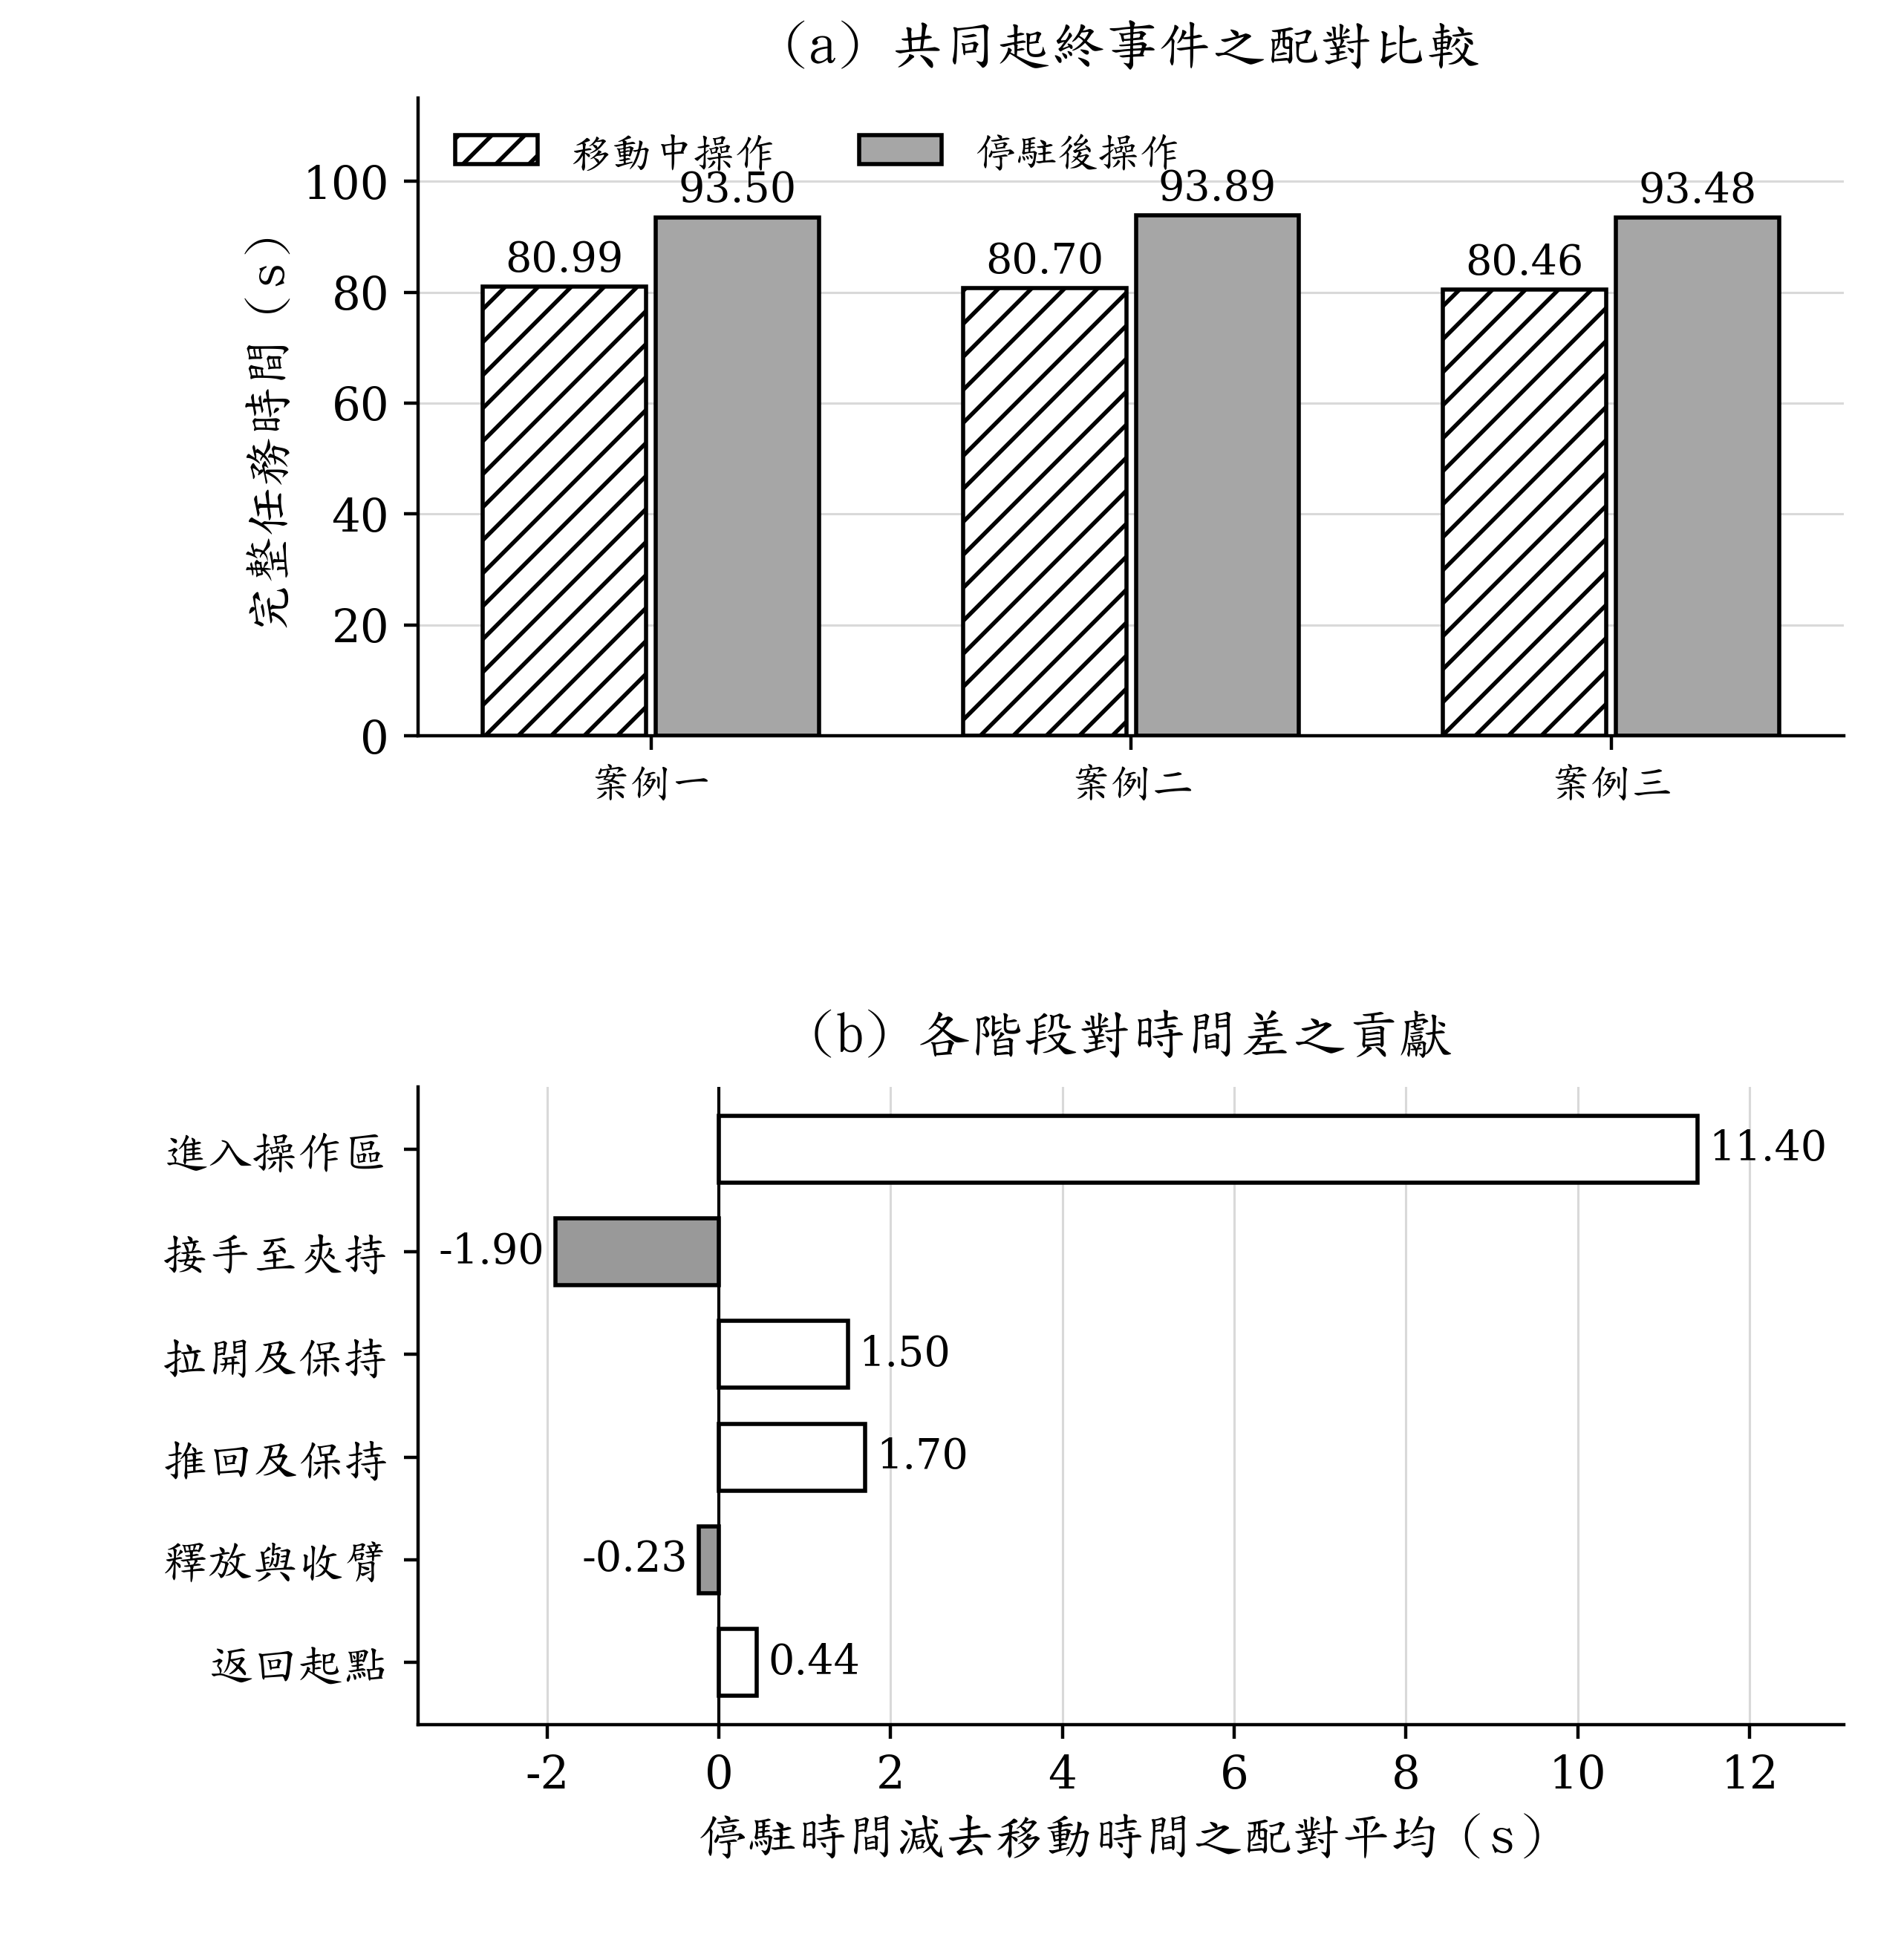
\includegraphics[width=0.98\textwidth]{figsrc/ch04/moving_parked_drawer_comparison.png}
    \caption{抽屜操作之策略比較：
    (a) 三組配對的完整任務時間；
    (b) 各階段之停駐時間減去移動時間的配對平均值。
    正值表示移動策略在該階段較省時，負值表示移動策略用時較長；
    各階段時間差之和對應完整任務的平均時間差。}
    \label{fig:ch4_moving_parked_drawer_comparison}
\end{figure}

拉開與開啟保持、推回與關閉保持兩段，
移動策略分別平均縮短約 $1.50$ 與 $1.70$ s；
釋放與收臂階段則平均增加約 $0.23$ s，
返回階段平均縮短約 $0.44$ s。
完整時間差主要來自進場與接手安排，
其次為開關抽屜期間的協同運動。

操作品質方面，六個案例在拉開階段的雙指接觸力皆持續達到 $0.5$ N，
但夾持期間最大相對位移的配對結果並未呈現相同方向。
移動策略的三個值為 $1.583$、$0.057$ 與 $0.251$ mm，
停駐策略則為 $0.092$、$0.095$ 與 $0.131$ mm，
兩組皆通過所設定的 $10$ mm 位移上限。
這些結果支持本組移動策略在完成既定操作條件下縮短完整任務時間，
夾持品質則須依其接觸與相對位移分別評估。
上述比較以三組配對案例描述本場景下的觀察，
後續住宅任務再檢查視覺目標、導航與多階段操作的整體銜接。

% ==================================================
% 4.5 住宅場景整合任務
% ==================================================
\section{住宅場景整合任務}
\label{sec:residential_integrated_task}

住宅任務將導航、視覺定位與機構操作串接於同一流程，
檢查控制器能否由不同感知目標與任務階段持續產生全身命令。
本節先以同一次含四名行人的完成案例，
說明開門、圓柱取物、抽屜取筆、收納及回程關門的執行結果，
再彙整無行人與含行人條件下的完成情形及策略比較。
持物與機構操作沿用第 3.6 節的固定相對位姿假設，
結果用於評估運動與任務銜接；摩擦抓持及滑移的適用範圍於第 4.6 節討論。

% ==================================================
% 4.5.1 視覺導引之開門與穿門
% ==================================================
\subsection{視覺導引之開門與穿門}
\label{subsec:residential_visual_door_passage}

機器人由臥室起點出發，先取得門把與門扇觀測，
再由時間對齊後的幾何量建立抓取位姿與底盤接近參考。
視覺前端使用機身與手腕相機的 RGB-D 資料，
RGB 影像進入實例分割，深度則用於目標幾何估測。
\cref{fig:ch4_residential_visual_observations}呈現同一案例在不同階段的目標影像。
門把、圓柱、抽屜把手與筆狀物件具有不同形狀及觀測距離，
各目標依第 3.5 節的幾何程序轉換為操作參考。

\begin{figure}[htbp]
    \centering
    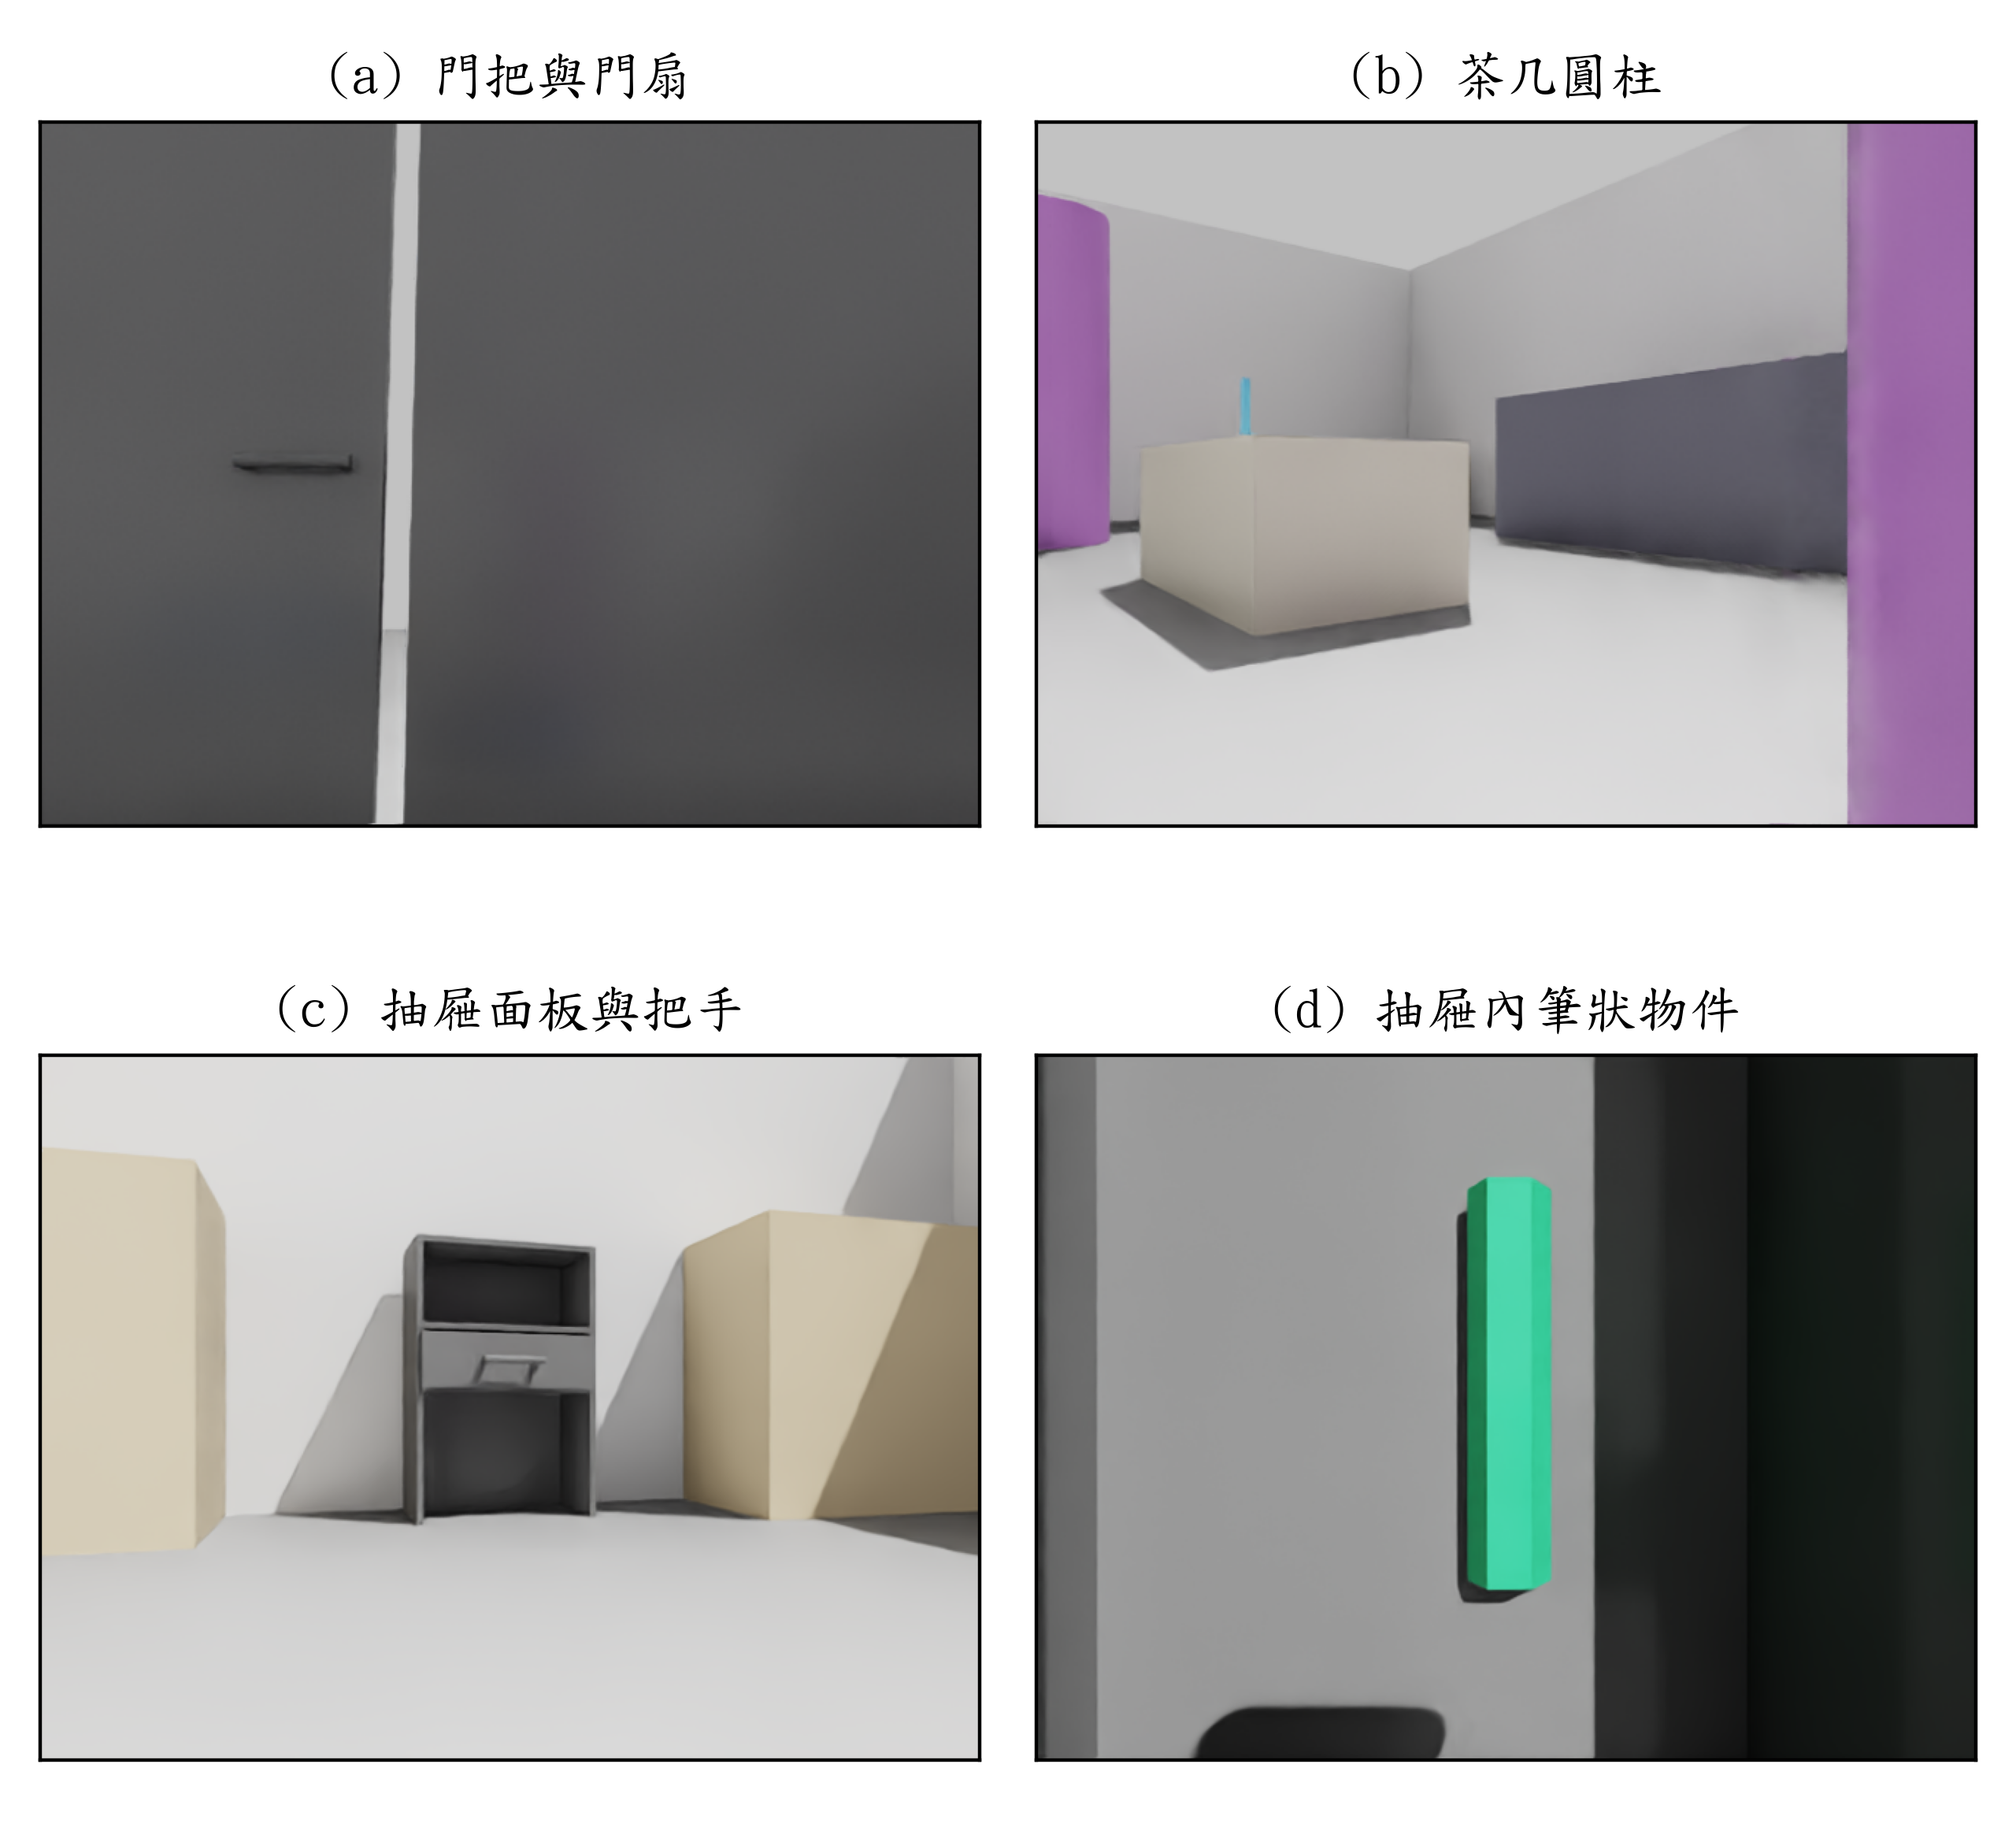
\includegraphics[width=0.98\textwidth]{figsrc/ch04/residential_visual_observations.png}
    \caption{住宅任務之 RGB 目標觀測：
    (a) 門把與門扇；(b) 茶几圓柱；
    (c) 抽屜面板與把手；(d) 抽屜內筆狀物件。
    (a)、(d) 為手腕相機影像，(b)、(c) 為機身相機影像。}
    \label{fig:ch4_residential_visual_observations}
\end{figure}

在此案例由控制接手至門把接近開始前的區間內，
共取得 $27$ 筆有效門把位置觀測。
以模擬幾何作離線對照，位置誤差中位數為 $1.41$ mm，
最大值為 $4.36$ mm。
這項統計對應該區間的有效幾何估測，
與影像分割準確度及後續末端追蹤誤差分別評估。
目標通過有效性與時間條件後，
底盤依導航參考接近，手臂同步展開並於末段併入世界座標抓取線。

抓持建立後，門角參考沿鉸鏈模型推進，
底盤與手臂共同配合把手的圓弧運動。
\cref{fig:ch4_residential_door_open_close}(a)顯示，
由控制接手至開門完成約需 $27.50$ s，門角達約 $85.02^\circ$。
解除抓持並確認手指張開後，
末端先退出門把，再銜接收臂與穿門導航。
此交接依實際執行回報推進，
使機器人在離開把手後才承接後續通行動作。

\begin{figure}[htbp]
    \centering
    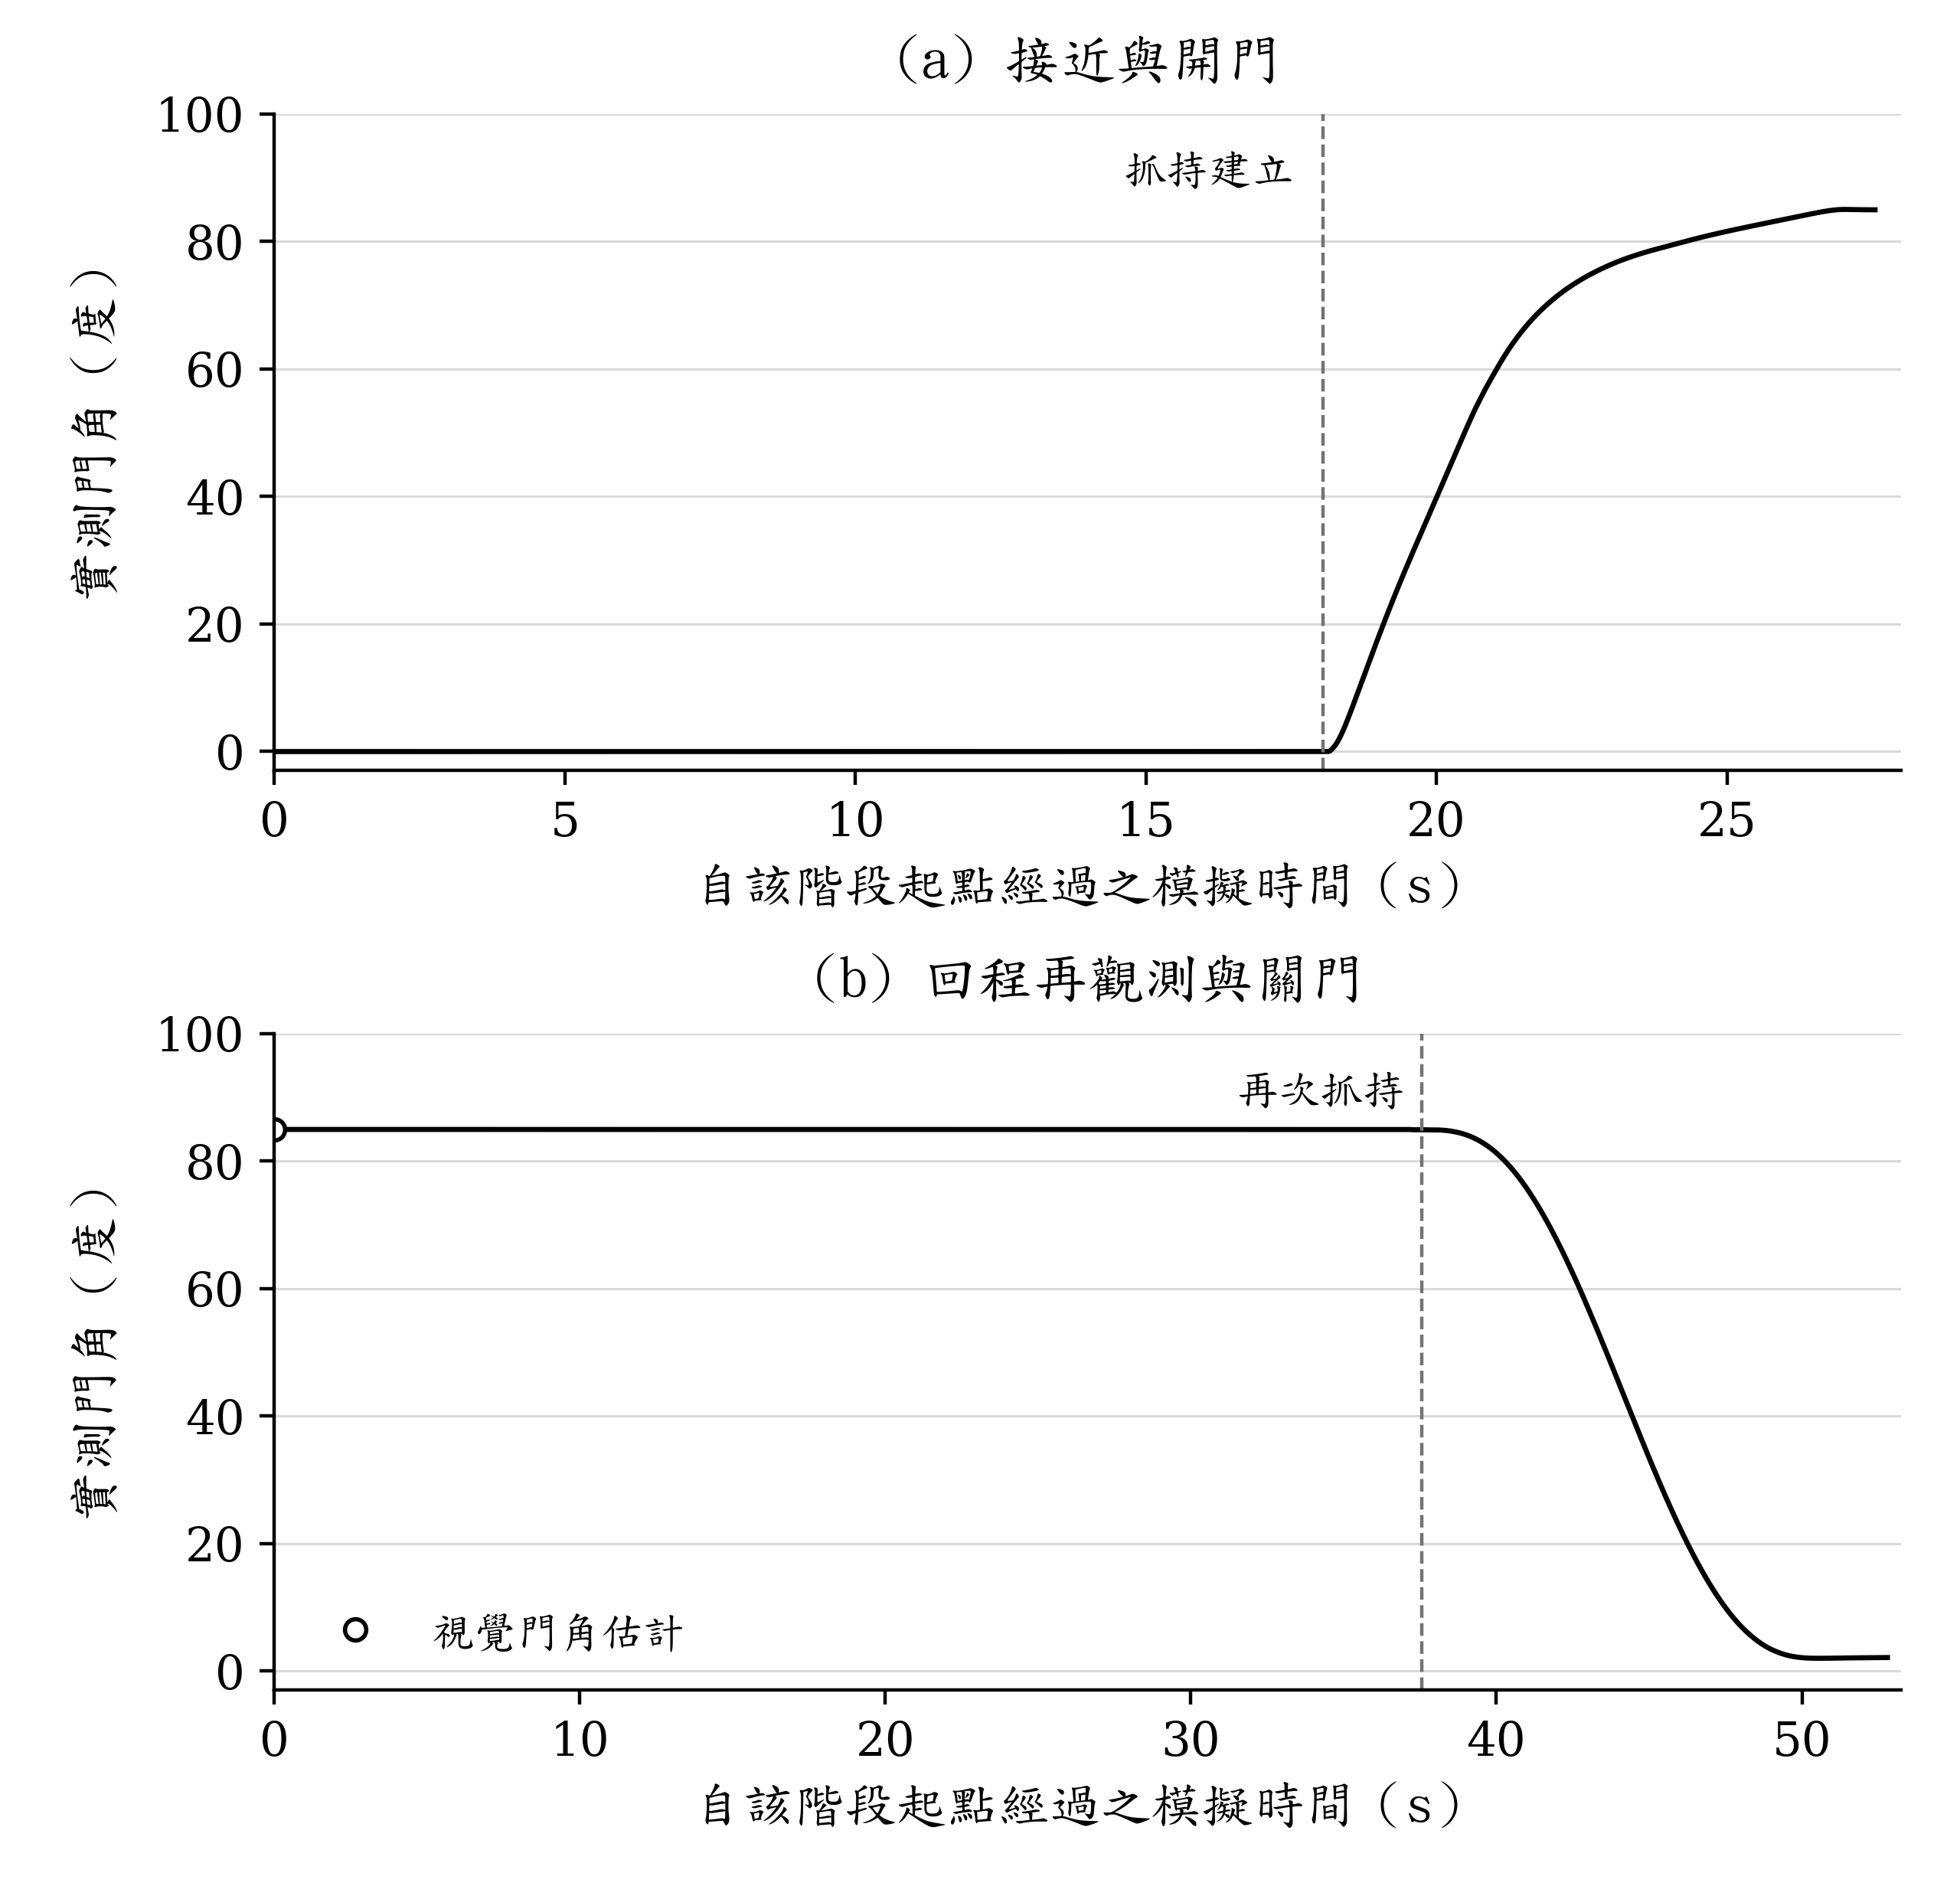
\includegraphics[width=0.98\textwidth]{figsrc/ch04/residential_door_open_close.png}
    \caption{同一次住宅任務之門扇操作：
    (a) 由控制接手至開門完成的實測門角；
    (b) 回程視覺再觀測至關門完成的實測門角。
    兩圖各由其階段起點計時，虛線標示抓持建立時刻；
    (b) 的空心圓為回程視覺門角估計。}
    \label{fig:ch4_residential_door_open_close}
\end{figure}

% ==================================================
% 4.5.2 茶几圓柱之移動中抓取與車尾收納
% ==================================================
\subsection{茶几圓柱之移動中抓取與車尾收納}
\label{subsec:residential_mobile_cylinder_storage}

通過門口後，機器人前往客廳茶几，
以圓柱觀測建立目標位置，再選擇具有導航可達性與連續手臂構型的操作區域。
本案例圓柱半徑為 $15$ mm、高度為 $200$ mm，
初始位置位於茶几側邊。
底盤接近時，手臂先依構型參考展開，
後段逐步轉為追蹤世界固定的抓取位置，
使底盤推進與末端接近在同一控制流程中重疊。

\cref{fig:ch4_residential_cylinder_mobile_pick}(a)呈現接近至收納期間的底盤速率。
由閉爪開始至抓持確認約為 $0.95$ s，
底盤累積移動約 $53.2$ mm，平均平移速率約為 $0.056$ m/s。
因此，此案例的閉爪與確認發生於底盤仍在移動的期間。
閉爪開始時，末端對操作參考的位置與姿態誤差分別約為 $4.45$ mm 與 $0.72^\circ$，
用於描述抓取銜接時的追蹤狀態。

\begin{figure}[htbp]
    \centering
    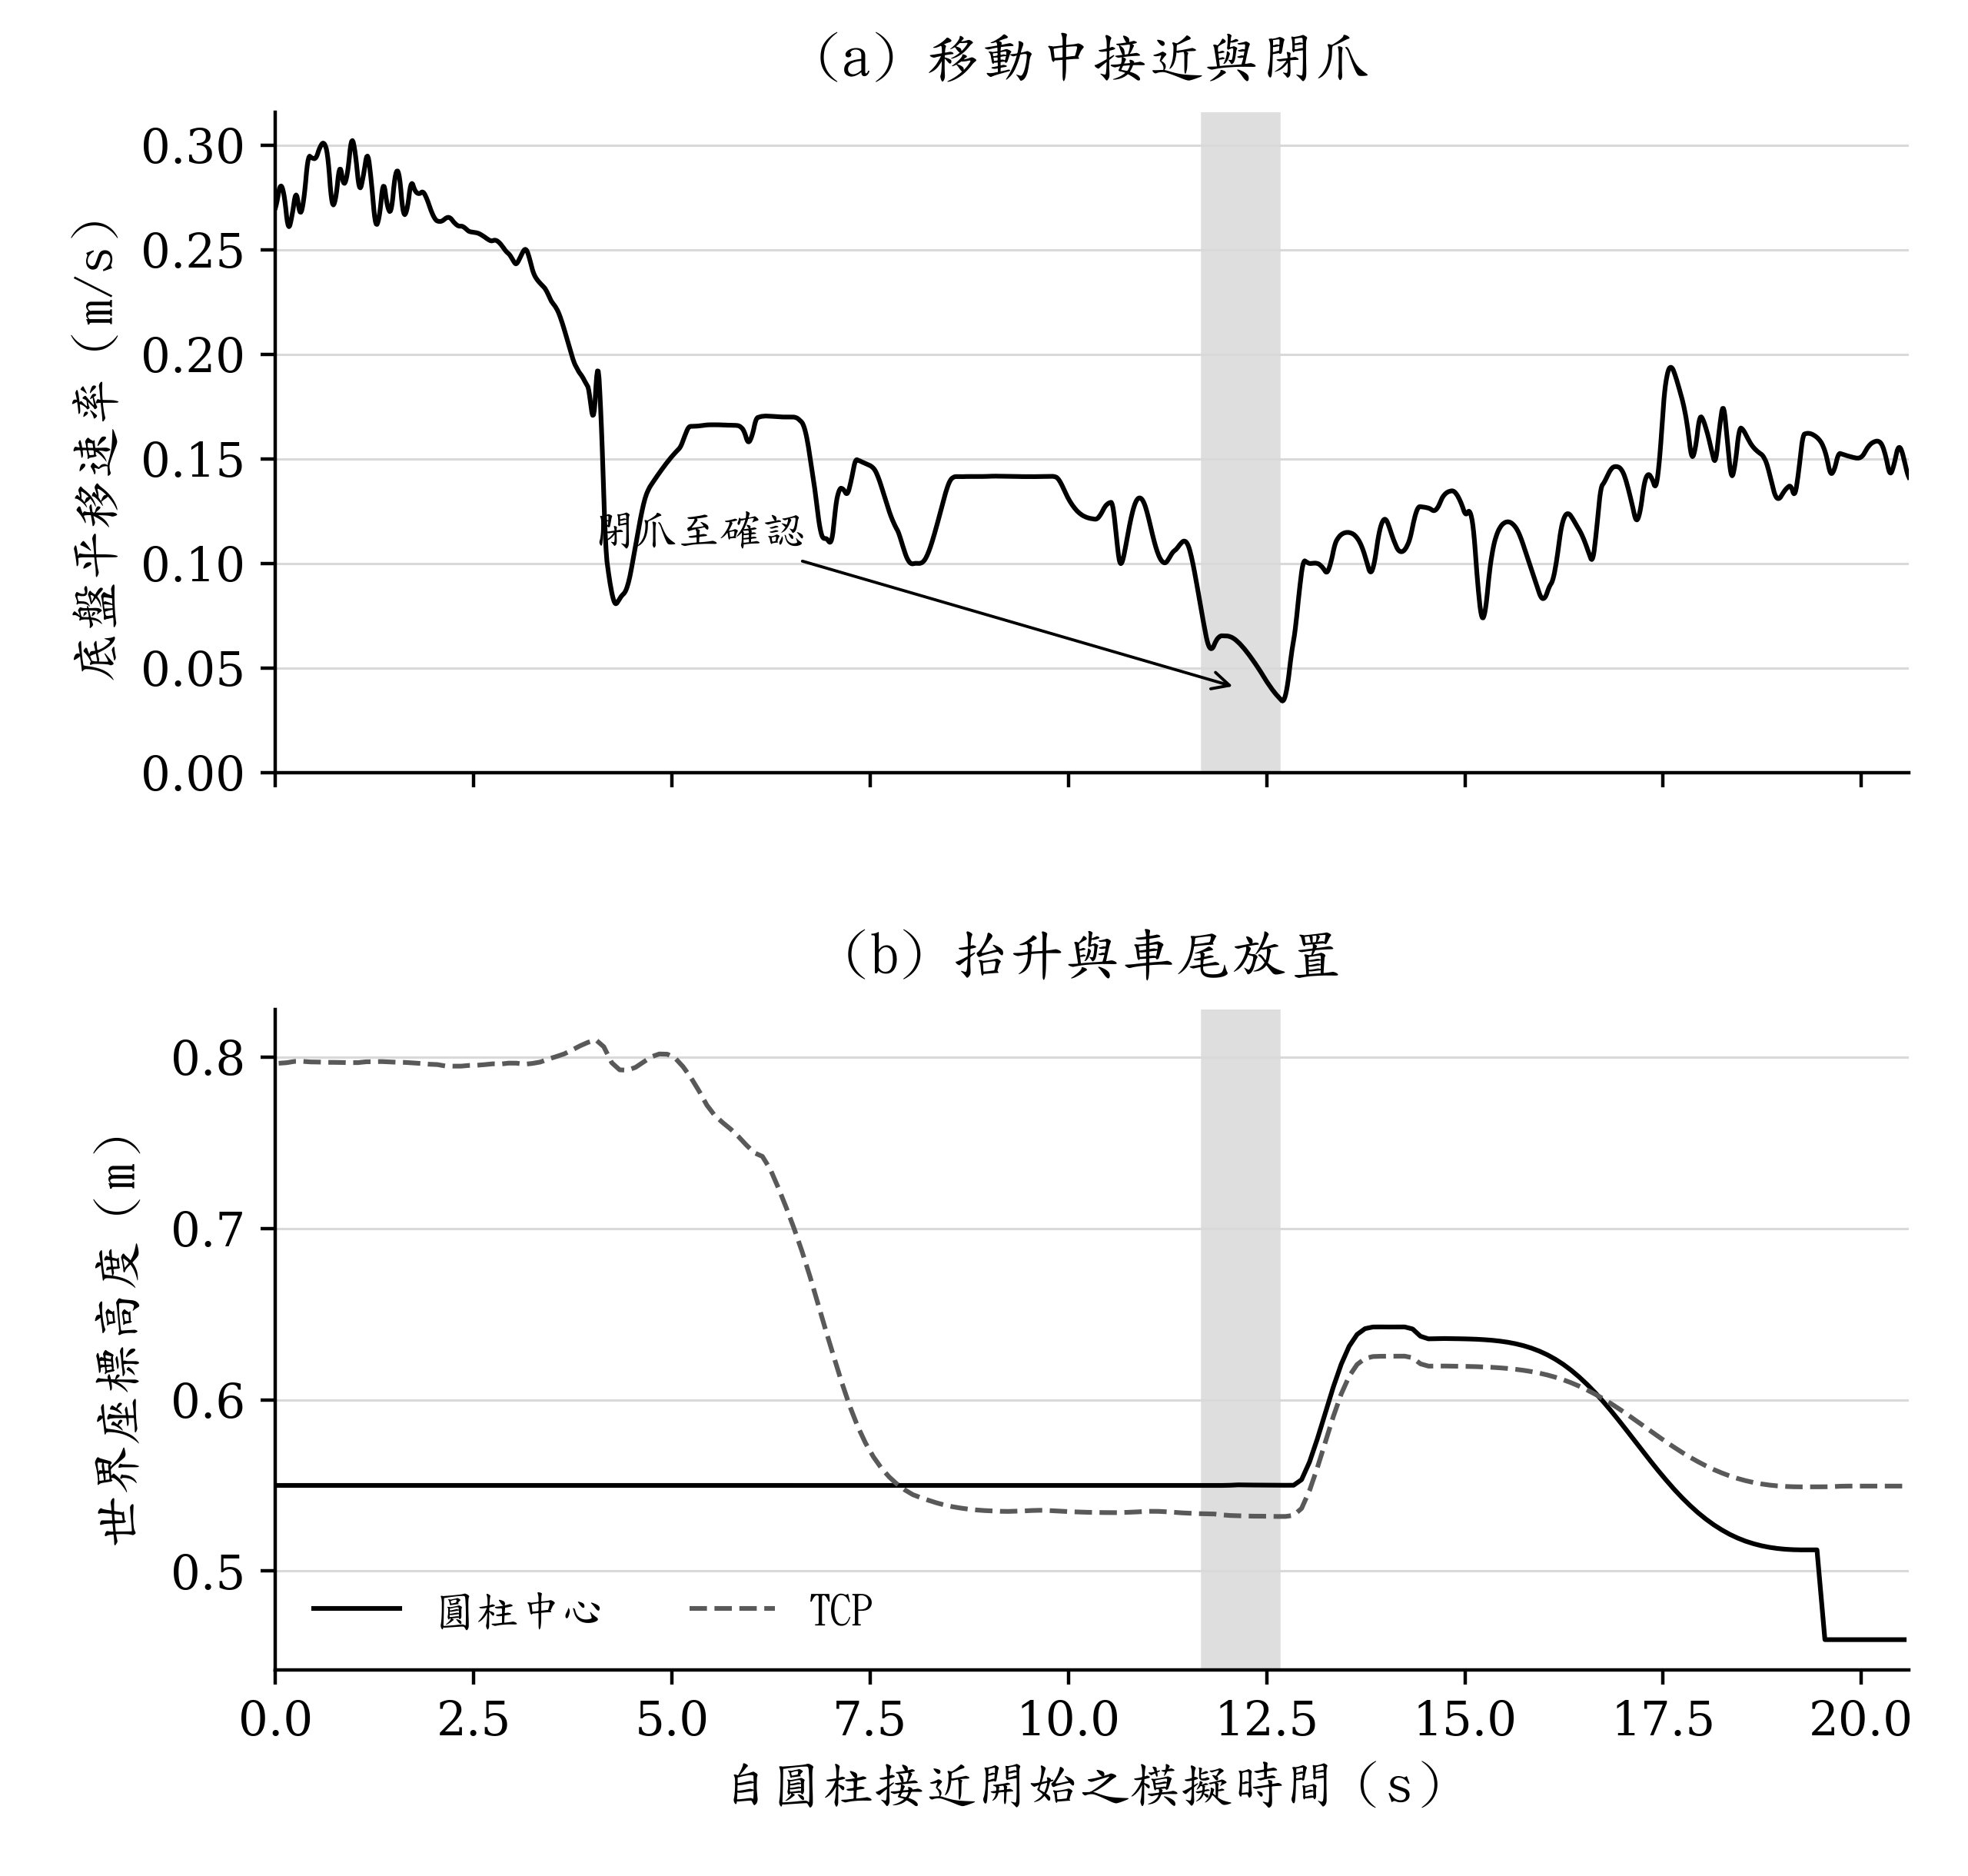
\includegraphics[width=0.98\textwidth]{figsrc/ch04/residential_cylinder_mobile_pick.png}
    \caption{住宅案例之圓柱移動中抓取與收納：
    (a) 底盤平移速率，以 $0.10$ s 位置差分計算；
    (b) 圓柱中心與 TCP 的世界座標高度。
    灰色區間為閉爪開始至抓持確認，兩圖使用相同時間基準。}
    \label{fig:ch4_residential_cylinder_mobile_pick}
\end{figure}

抓持確認後，末端參考轉為底盤相對目標，
接續抬升、移向車尾盒上方、釋放與收臂。
\cref{fig:ch4_residential_cylinder_mobile_pick}(b)顯示物件隨抬升離開桌面，
再於車尾放置階段降低高度。
放置時先完成解除抓持的執行確認，再張爪並等待物件落下，
後續由實際構型建立收臂參考。
任務結束時另以物件中心在盒體座標中的位置核對收納結果，
避免僅由放置階段事件推定物件已留在盒內。

% ==================================================
% 4.5.3 開抽屜取筆、收納與關閉抽屜
% ==================================================
\subsection{開抽屜取筆、收納與關閉抽屜}
\label{subsec:residential_drawer_marker_storage}

圓柱收納後，機器人前往右側房間的抽屜櫃。
家具登錄位置提供搜尋先驗，當次面板與把手觀測則用於修正操作幾何。
此案例的實際抽屜位置相對登錄位置偏移約 $44.7$ mm，
朝向差為 $2^\circ$；融合五筆觀測後，
所估櫃體平面位置與模擬幾何的差約為 $7.8$ mm。
控制端依更新後的滑軌方向建立接近、拉開及後續選位參考。

抓住把手後，抽屜沿滑軌拉出至約 $200$ mm。
\cref{fig:ch4_residential_drawer_pick_close}(a)顯示完整開度歷程，
(b)則比較拉開期間的底盤軸向平移與抽屜開度變化。
兩者具有相近的位移趨勢，
表示底盤移動承接此階段主要的滑軌方向運動，
手臂持續配合末端位姿與構型需求。
拉開結束且解除抓持時，控制端估計開度為 $200.50$ mm，
對應的模擬實測開度為 $200.29$ mm。

\begin{figure}[htbp]
    \centering
    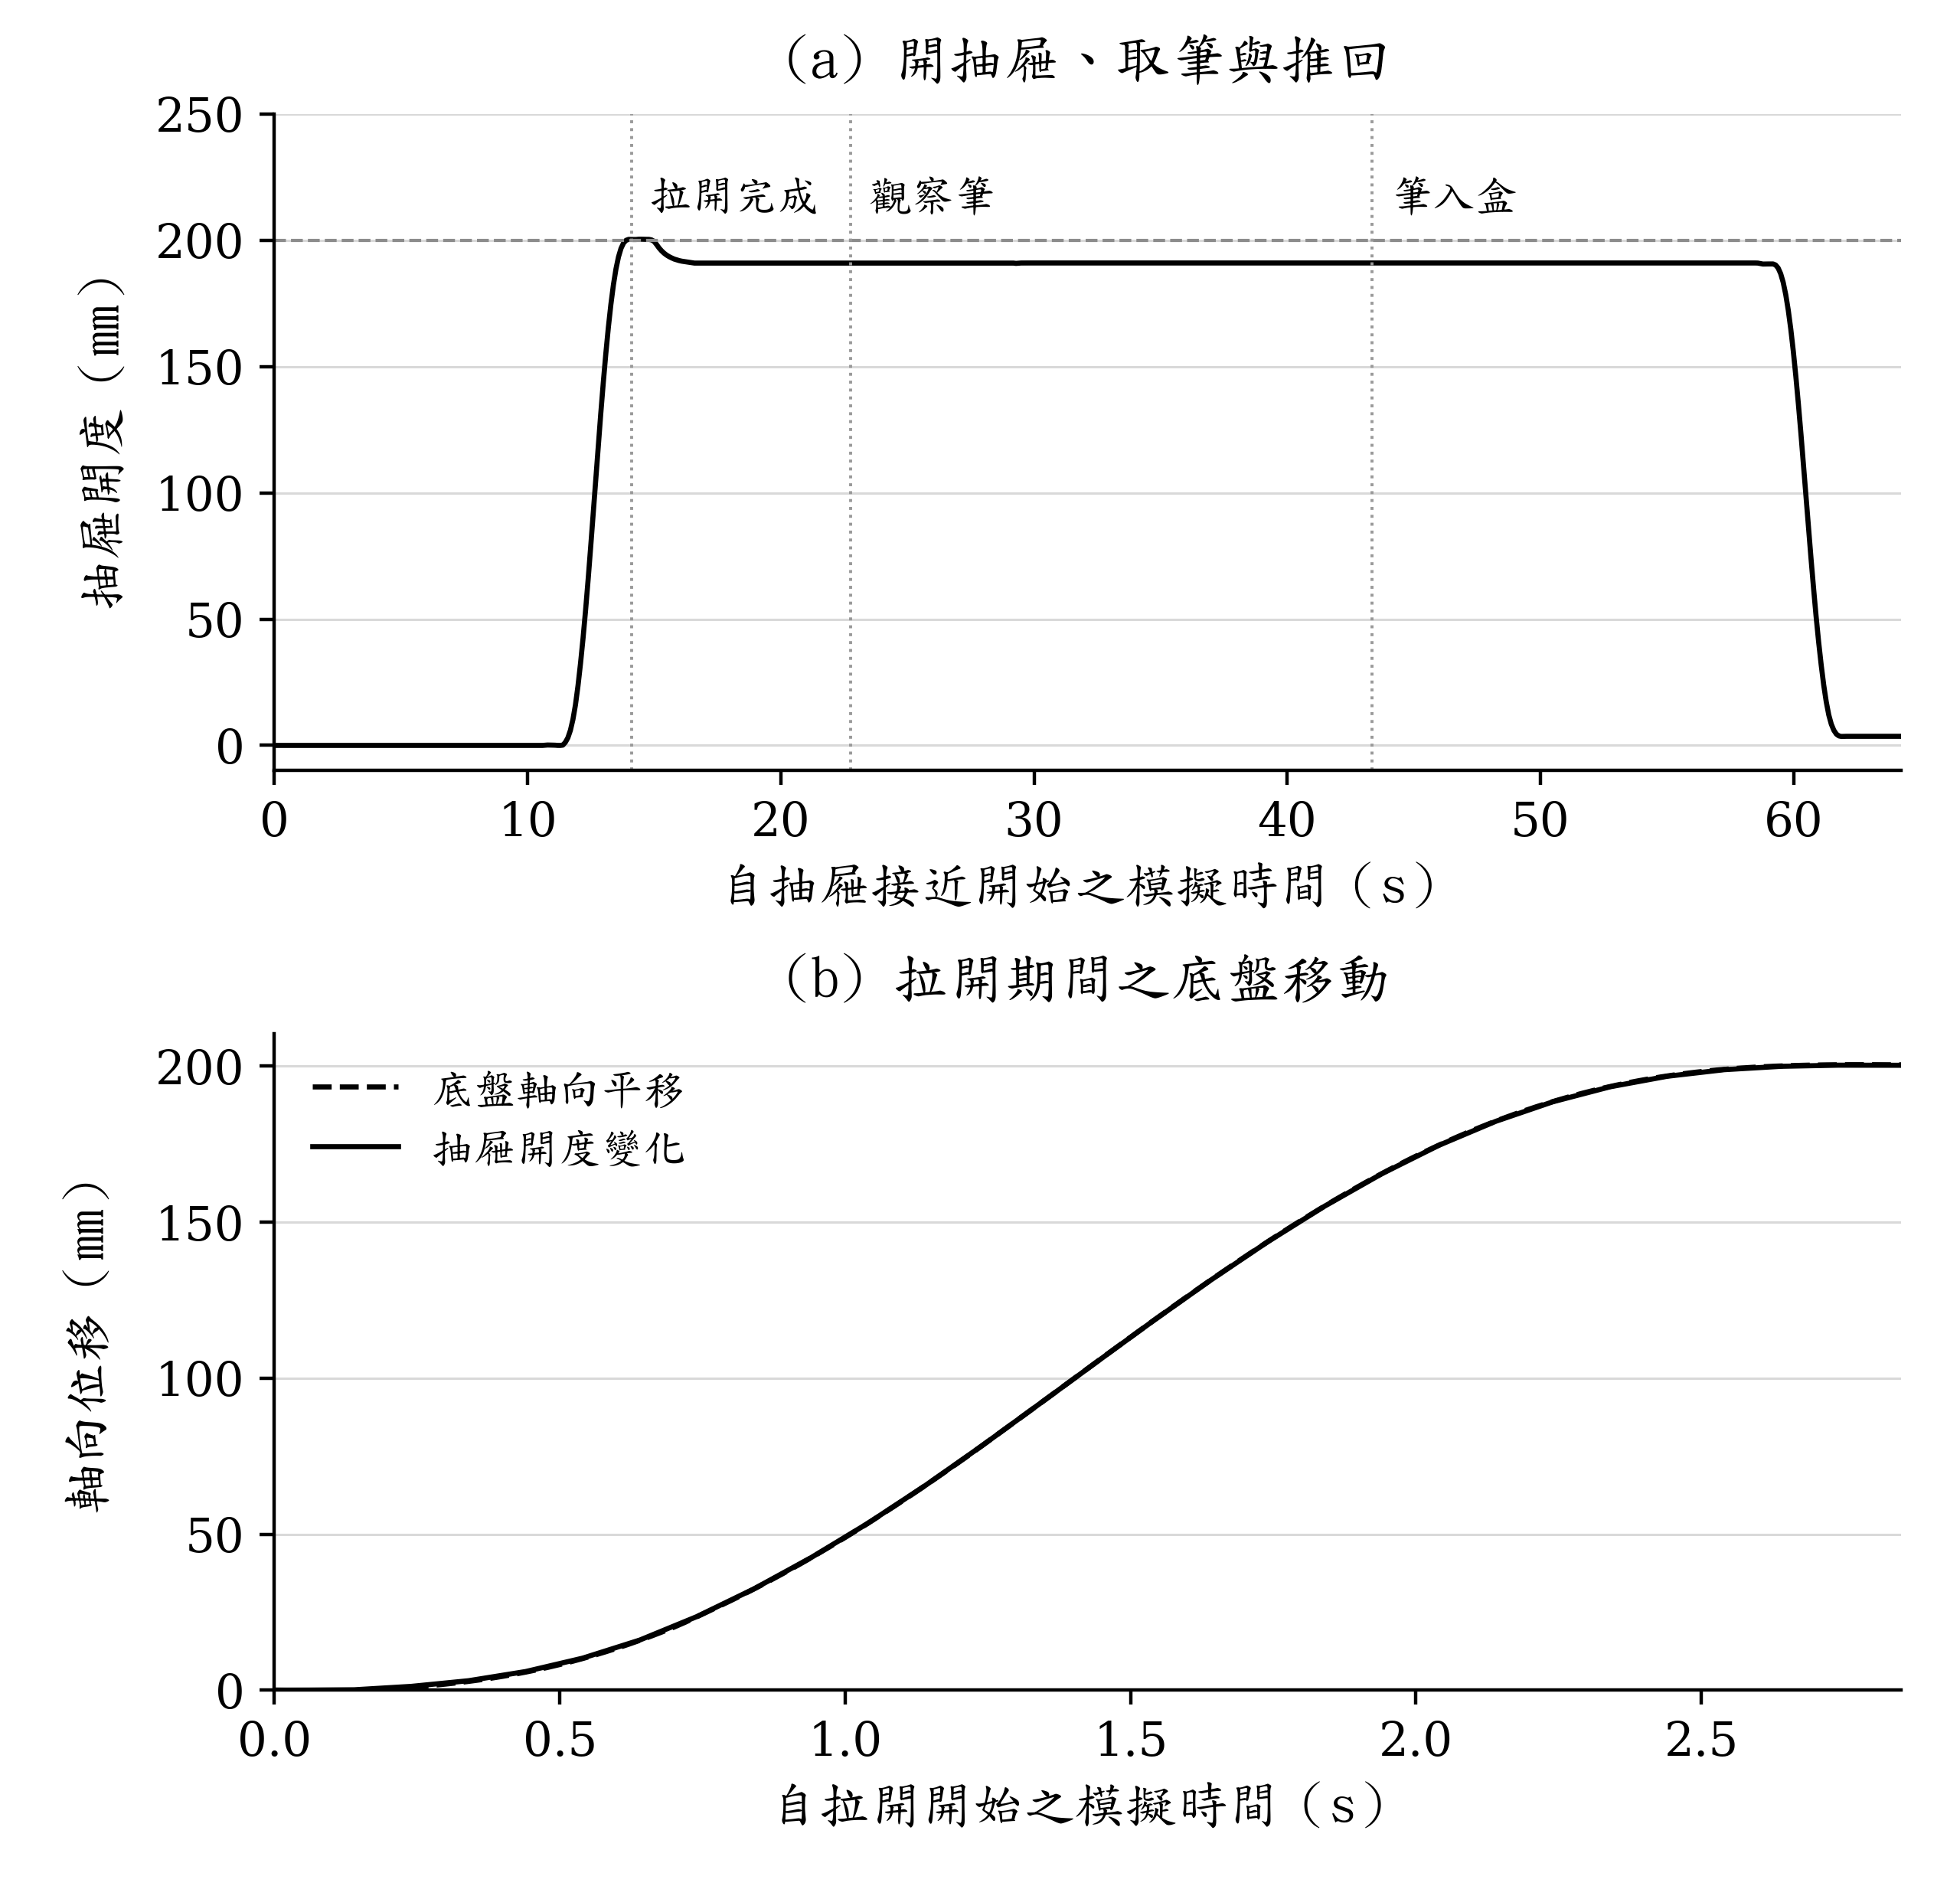
\includegraphics[width=0.98\textwidth]{figsrc/ch04/residential_drawer_pick_close.png}
    \caption{住宅案例之抽屜操作：
    (a) 自把手接近開始至關抽屜完成的實測開度，水平虛線為 $200$ mm；
    (b) 拉開期間的底盤軸向平移與抽屜開度變化。
    (a) 的垂直點線標示拉開完成、觀察筆與筆入盒事件，
    (b) 的位移由拉開起點計算。}
    \label{fig:ch4_residential_drawer_pick_close}
\end{figure}

解除把手抓持後，手臂轉至抽屜上方的觀察構型，
再由筆狀物件的遮罩、深度與主軸估測建立抓取位姿。
本實驗使用長度約 $140$ mm 的粗筆狀代理物，
抓取方向依主軸與可行手臂構型選擇。
完成接近與抬升後，先退出抽屜附近空間，
再銜接車尾收納及收臂。
以圓柱入盒事件至筆入盒事件計算，
此區間共需 $75.60$ s，涵蓋兩操作區之間的導航、
把手定位、開抽屜、觀察、取筆與放置。

關抽屜前重新觀測把手，依更新位置修正推回起點，
再由相同滑軌方向建立反向運動參考。
推回結束且解除抓持時，控制端估計剩餘開度約為 $4.74$ mm，
模擬實測值約為 $3.58$ mm；整體任務結束時為 $3.61$ mm。
推回參考在關閉端預留 $5$ mm 行程，
因此本案例以接近關閉位置作為終點，保留與機構硬限位之間的餘量。

% ==================================================
% 4.5.4 回程通行、關門與返回起點
% ==================================================
\subsection{回程通行、關門與返回起點}
\label{subsec:residential_return_door_closing}

完成關抽屜後，機器人沿導航路徑返回門口。
本案例回程時門扇仍維持約 $85^\circ$，
先由視覺再觀測門角，通過既有開口後，再接近臥室側的把手操作位置。
回程視覺門角估計為 $84.876^\circ$，
同一觀測時刻的模擬實測值約為 $84.932^\circ$，差約 $0.056^\circ$。
新的把手目標由該門角與鉸鏈幾何重建，
使回程接近能對應當時的門扇狀態。

再次抓持後，底盤與手臂依繞鉸鏈的共轉參考執行關門。
\cref{fig:ch4_residential_door_open_close}(b)顯示，
抓持前門角維持穩定，操作開始後逐步減少至約 $2^\circ$。
解除抓持時的實測門角約為 $1.99^\circ$，
完成張爪與末端退出後約為 $2.11^\circ$。
此階段結束後，機器人收臂並返回起點，
終點與起始位置的平面距離約為 $0.134$ m，
符合本組整合任務所使用的 $0.60$ m 返回範圍。

\cref{tab:ch4_residential_terminal_states}整理代表案例的終態。
圓柱與筆狀物件均位於收納判定範圍，
抽屜與門扇停在所設定的近關閉位置，
底盤亦返回起點附近。
物件入盒判定使用其中心位置，
門角與抽屜開度則由模擬機構狀態另行核對。
表中物件位置以收納盒所屬之 \texttt{base\_link} 座標表示。

\begin{table}[htbp]
    \centering
    \caption{住宅代表案例之任務終態核對}
    \label{tab:ch4_residential_terminal_states}
    \begingroup
    \small
    \renewcommand{\arraystretch}{1.25}
    \begin{tabular}{p{0.21\textwidth} p{0.40\textwidth} p{0.25\textwidth}}
        \hline
        項目 & 任務結束時之量測 & 核對內容 \\
        \hline
        圓柱中心 & $(-0.140,\ 0.024,\ 0.301)$ m & 位於收納範圍 \\
        筆狀物件中心 & $(-0.095,\ 0.039,\ 0.299)$ m & 位於收納範圍 \\
        抽屜剩餘開度 & $3.61$ mm & 接近關閉位置 \\
        門扇角度 & $2.17^\circ$ & 接近 $2^\circ$ 參考 \\
        底盤返回距離 & $0.134$ m & 小於 $0.60$ m \\
        \hline
    \end{tabular}
    \endgroup
\end{table}

% ==================================================
% 4.5.5 任務銜接與整體完成情形
% ==================================================
\subsection{任務銜接與整體完成情形}
\label{subsec:residential_task_completion}

\cref{fig:ch4_residential_mission_timeline}將上述操作放回同一任務的底盤軌跡與時間軸。
由控制接手至返回完成共需約 $335.3$ s，皆以模擬時間計算，
交權前的起動準備另行保留。
依開門完成、圓柱入盒、筆入盒、關抽屜、關門與返回等事件切分，
六段時間依序約為 $27.5$、$71.1$、$75.6$、$20.9$、$110.7$ 與 $29.5$ s。
各段包含相應的導航、操作與等待，
因此其長度同時反映路線、觀測及階段銜接的影響。

\begin{figure}[htbp]
    \centering
    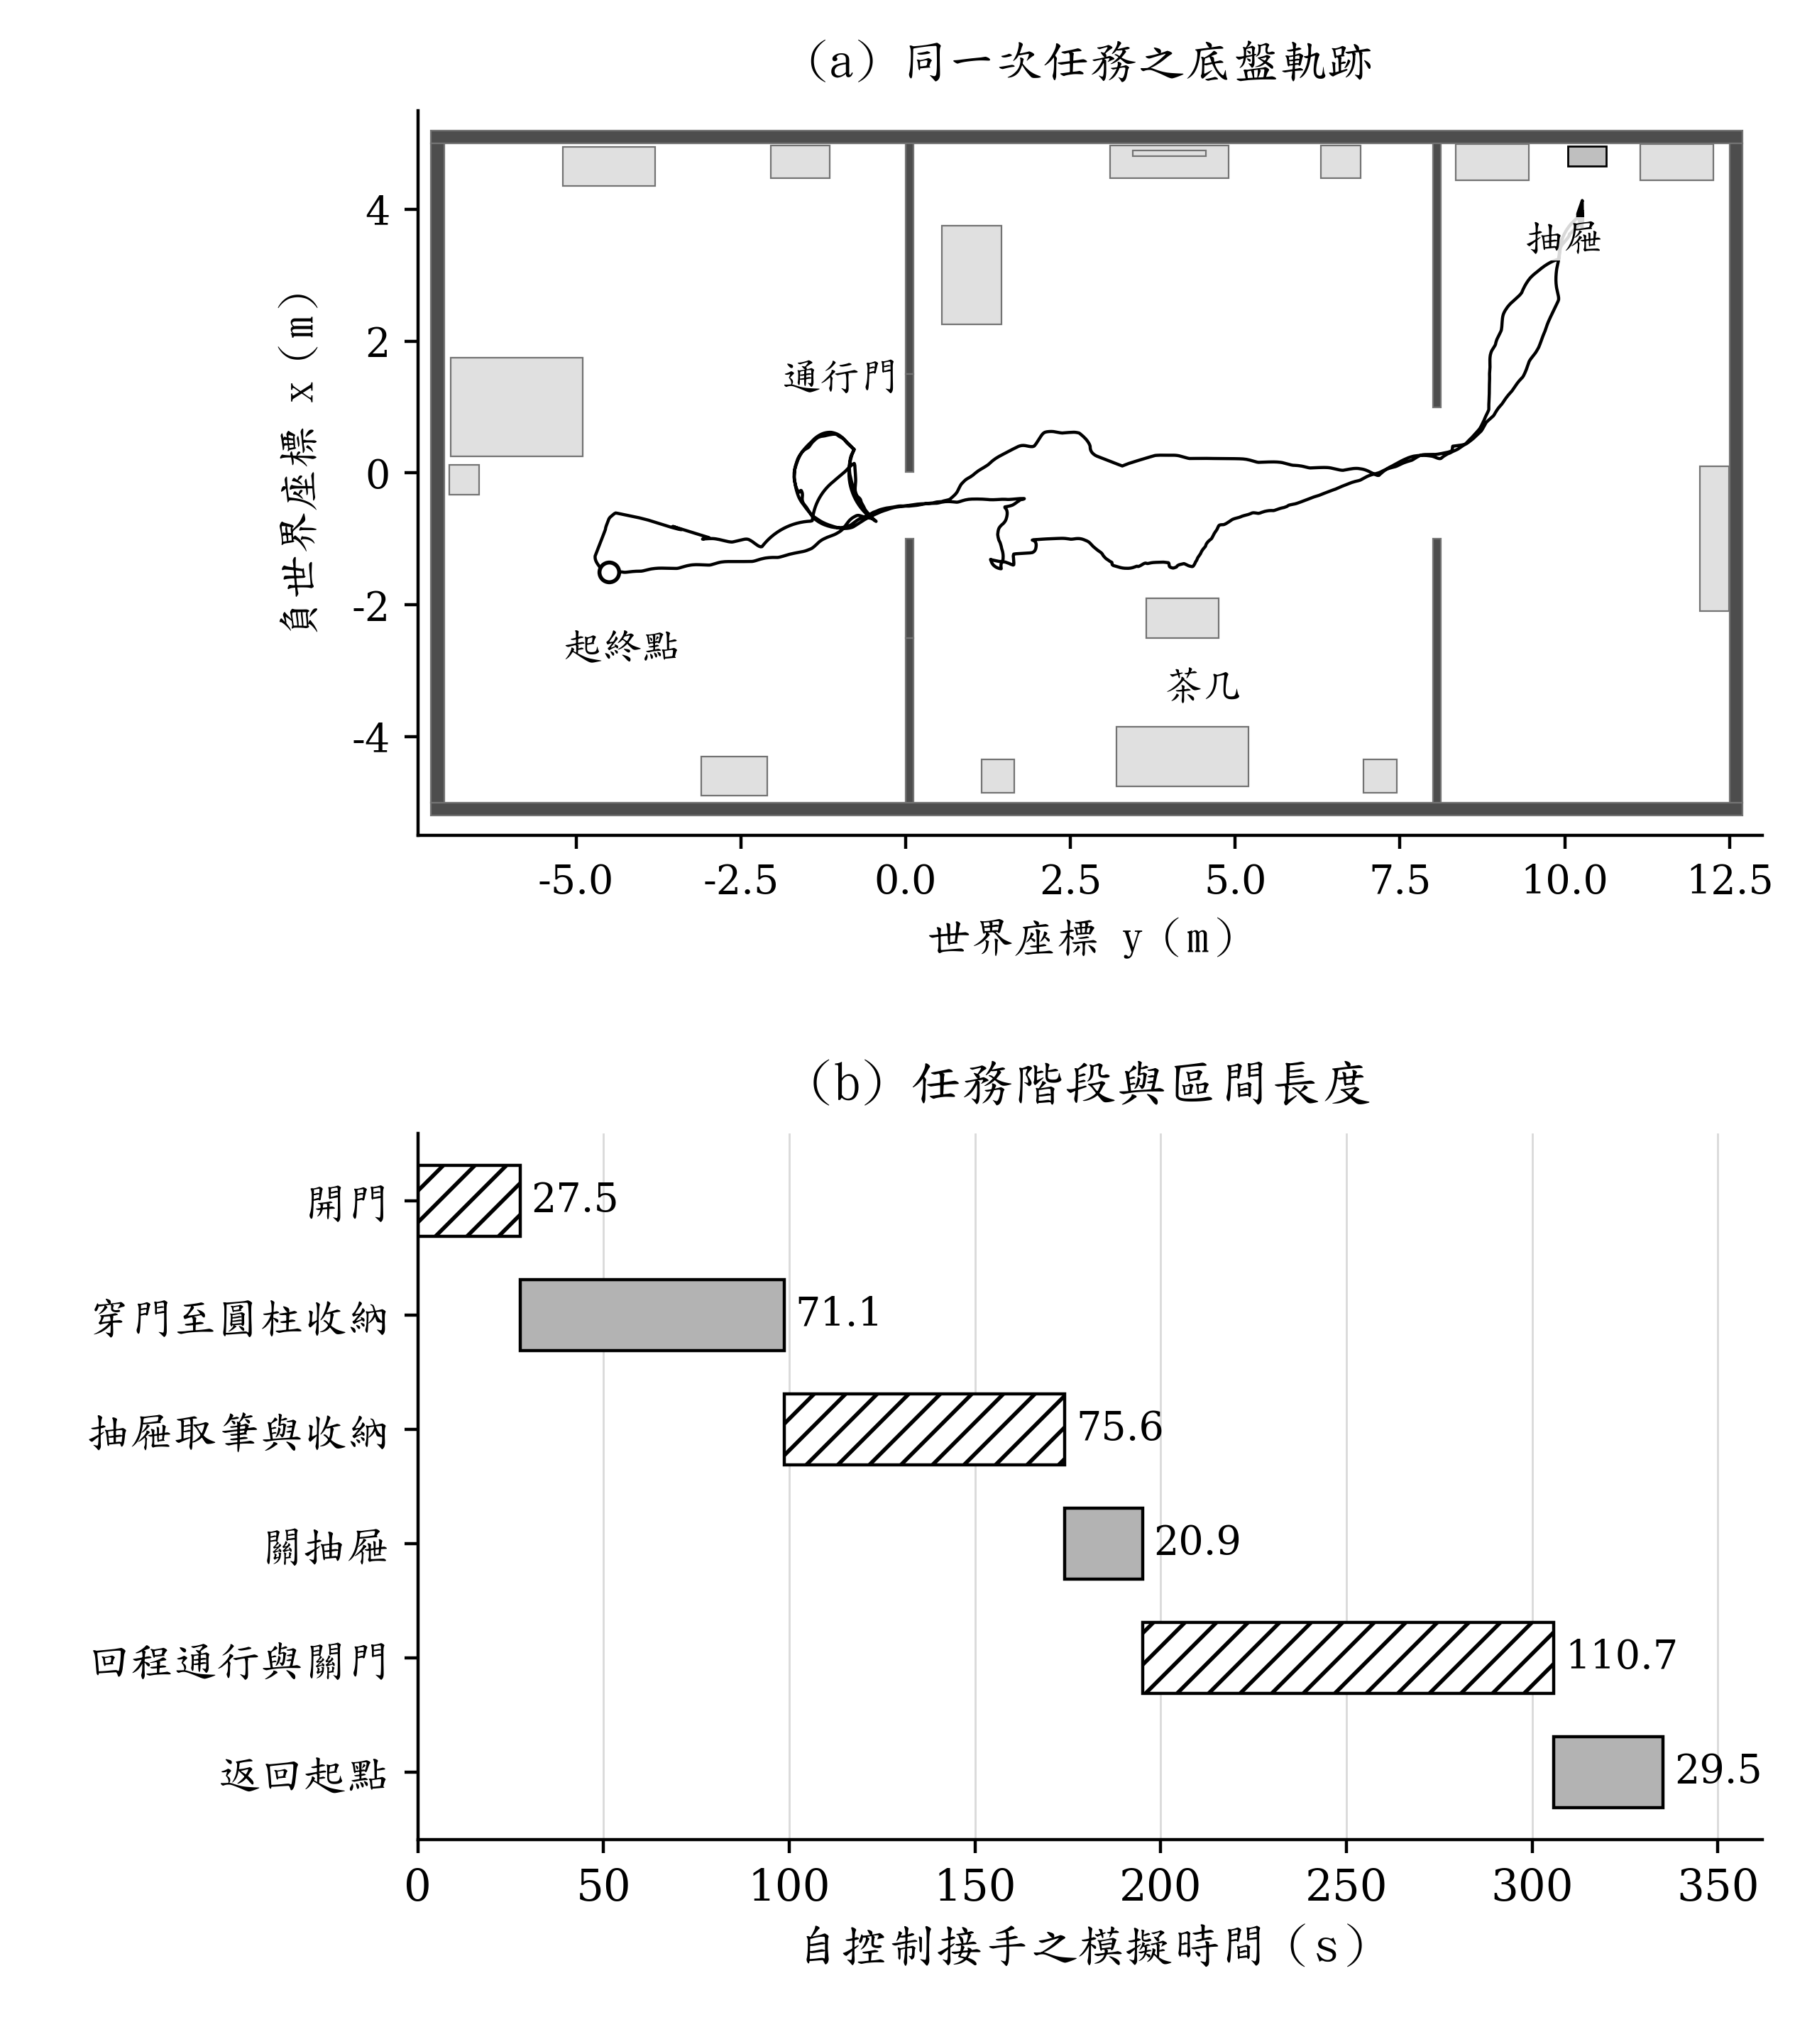
\includegraphics[width=0.98\textwidth]{figsrc/ch04/residential_mission_trajectory_timeline.png}
    \caption{同一次住宅整合任務之運動與階段銜接：
    (a) 底盤軌跡與固定場景底圖，空心圓為起點；
    (b) 由控制接手起算的任務時間軸，條形旁數值為各區間長度，單位為秒。}
    \label{fig:ch4_residential_mission_timeline}
\end{figure}

除代表案例外，另彙整 $43$ 次住宅整合紀錄，
其中無行人條件為 $27$ 次，含行人條件為 $16$ 次。
含行人場景配置四名移動物件，
並保留其接近機器人時的暫停讓行規則。
\cref{tab:ch4_residential_completion_counts}列出完成與未完成數。
完成判定要求具有回程關門及兩次收納事件，
底盤終點位於返回範圍；完成案例另核對兩物件的終態收納位置。
這批紀錄包含整合期間的控制與交接修正，
完成數用於描述所測流程，不作為固定版本的成功率估計。

\begin{table}[htbp]
    \centering
    \caption{住宅整合紀錄之完成情形}
    \label{tab:ch4_residential_completion_counts}
    \begingroup
    \small
    \renewcommand{\arraystretch}{1.25}
    \begin{tabular}{l l c c c}
        \hline
        環境條件 & 接近策略 & 紀錄數 & 完成數 & 未完成數 \\
        \hline
        無行人 & 移動中操作 & $15$ & $9$ & $6$ \\
        無行人 & 停駐後操作 & $12$ & $9$ & $3$ \\
        含行人 & 移動中操作 & $8$ & $4$ & $4$ \\
        含行人 & 停駐後操作 & $8$ & $7$ & $1$ \\
        \hline
    \end{tabular}
    \endgroup
\end{table}

策略時間比較採用無行人條件下，兩種策略皆有完成案例的八個圓柱位置種子。
住宅停駐策略先完成接近前的停車，再展臂與接近；
後續機構操作仍允許全身協同運動，
與第 4.4 節的全區間底盤保持對照分別解讀。
同一種子與策略若有重複完成紀錄，先取其平均，
再對八個種子等權平均，以避免重複次數影響整體權重。

\cref{fig:ch4_residential_strategy_comparison}(a)顯示各種子的條件時間比較。
移動與停駐策略的平均時間分別為 $319.25$ 與 $337.53$ s，
差約 $18.28$ s，相對縮短約 $5.42\%$。
此數值限於已完成案例，需連同前述未完成紀錄及版本條件解讀。
含行人條件的交會時間會隨任務推進改變，
且兩組完成的種子集合不同，因此其完成情形另列，
不與無行人的時間平均值混合。

\begin{figure}[htbp]
    \centering
    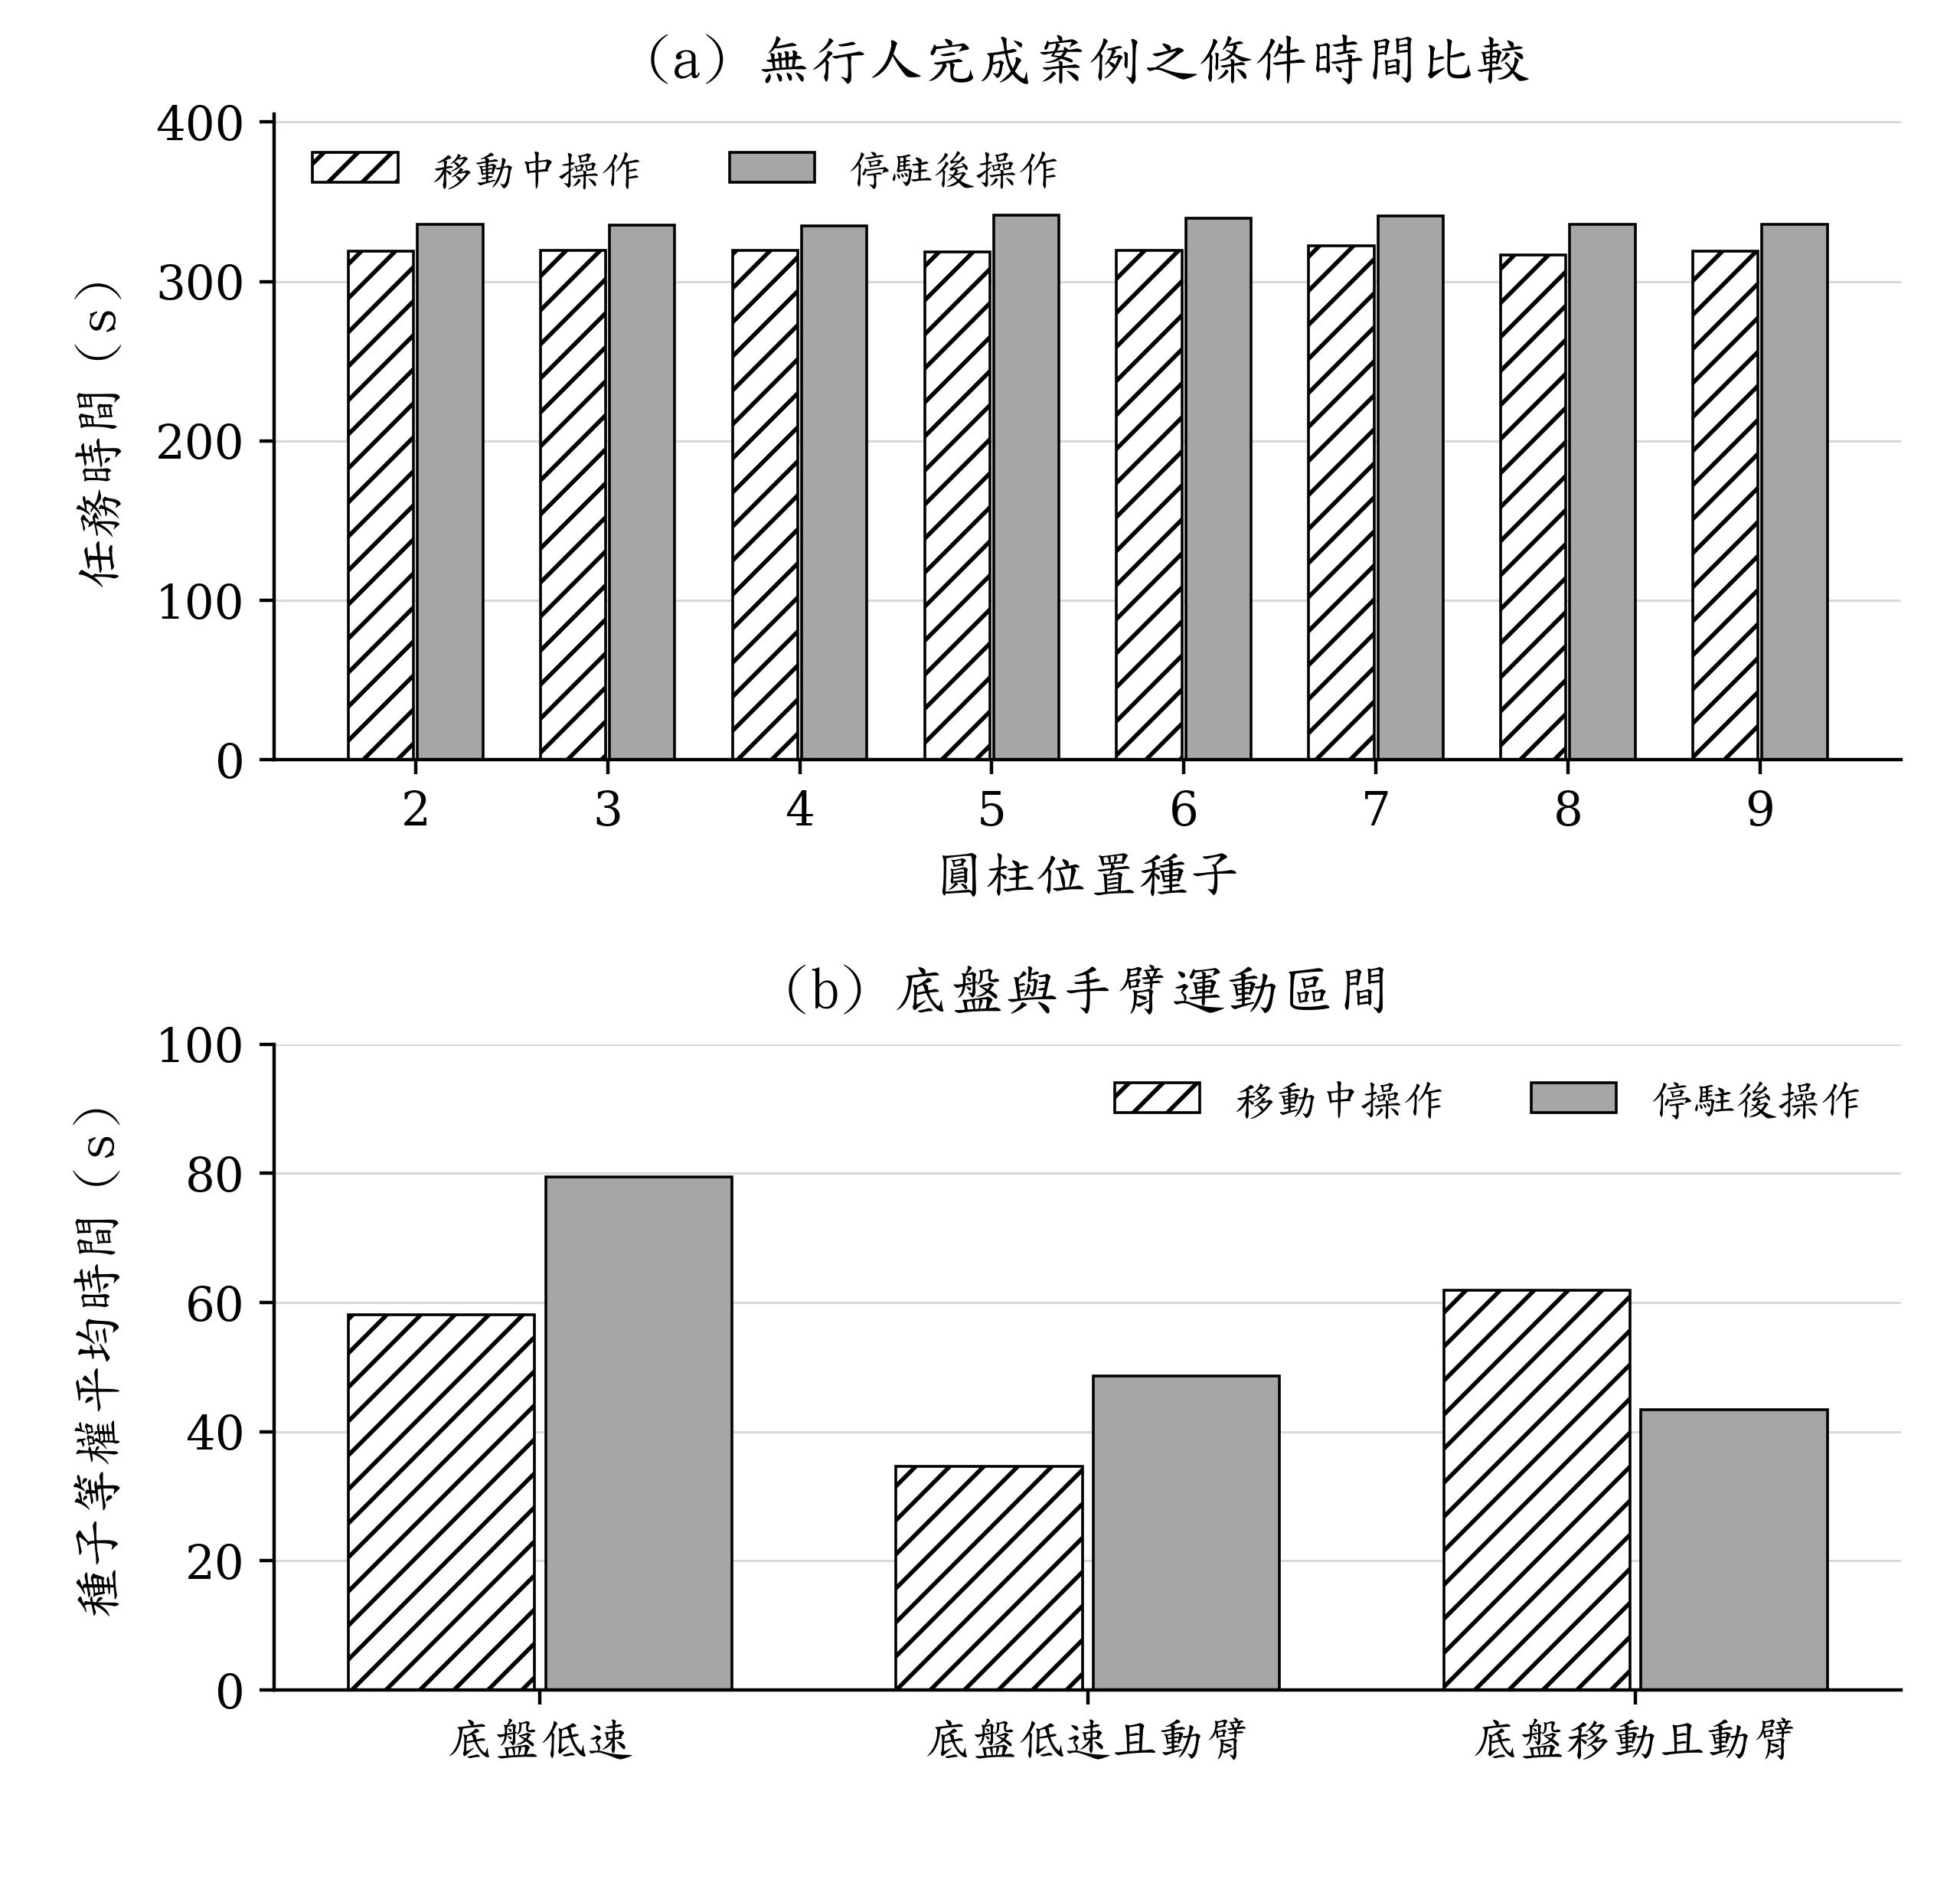
\includegraphics[width=0.98\textwidth]{figsrc/ch04/residential_strategy_seed_comparison.png}
    \caption{無行人住宅任務之完成案例比較：
    (a) 八個圓柱位置種子下的任務時間；
    (b) 底盤低速、低速且動臂及移動且動臂的種子等權平均時間。
    同一種子與策略的重複完成紀錄先取平均；
    低速且動臂為低速區間的子集合，各類時間不相加為任務總時間。}
    \label{fig:ch4_residential_strategy_comparison}
\end{figure}

運動重疊區間由 $50$ ms 取樣的位姿與關節差分判定。
底盤低速條件為平移速率小於 $0.01$ m/s 且偏航速率小於 $0.02$ rad/s；
動臂條件為六軸關節速度向量範數大於 $0.05$ rad/s；
底盤移動且動臂另要求平移速率大於 $0.03$ m/s。
依此定義，移動策略的平均底盤低速時間由 $79.39$ 降至 $58.14$ s，
低速且動臂時間由 $48.60$ 降至 $34.61$ s，
移動且動臂時間則由 $43.44$ 增至 $61.90$ s，
如\cref{fig:ch4_residential_strategy_comparison}(b)所示。
這些結果呈現接近與手臂運動重疊對任務時間安排的影響，
其追蹤品質、計算期限及中止原因仍需配合個別紀錄分析。

% ==================================================
% 4.6 計算效能、失敗案例與研究限制
% ==================================================
\section{計算效能、失敗案例與研究限制}
\label{sec:performance_failures_limits}

前述實驗分別呈現模型預測、導航與全身操作的結果，
其實際表現亦受到計算時間、命令承接與量測條件影響。
本節先以第 4.5 節的住宅代表案例分析計算耗時與控制期限，
再由相同整合紀錄集合整理未完成情形，
最後界定感知、接觸、幾何檢查及任務統計的適用範圍。
各項結果依對應的時間來源與評估條件解讀。

% ==================================================
% 4.6.1 求解時間與控制期限分析
% ==================================================
\subsection{求解時間與控制期限分析}
\label{subsec:solver_timing_deadline_analysis}

住宅案例的物理模擬、視覺推論、導航前端與控制工作程序同時執行。
計算耗時以主機時鐘量測，
並區分工作程序計算與派工至結果接收的來回時間：
\begin{equation}
    T_{\mathrm{rt}}
    =T_{\mathrm{in}}+T_{\mathrm{comp}}+T_{\mathrm{out}}.
    \label{eq:ch4_control_roundtrip_time}
\end{equation}
其中 $T_{\mathrm{in}}$ 包含輸入傳遞及等待工作程序開始的時間，
$T_{\mathrm{comp}}$ 為該次工作程序的計算時間，
$T_{\mathrm{out}}$ 為結果傳遞與接收時間。
工作程序另包含參考處理、最佳化、候選及停止軌跡核對等運算，
因此其耗時範圍大於單一 QP 數值求解。

\cref{tab:ch4_control_runtime}列出保存來回耗時的 $6688$ 筆回覆。
區段依控制模式劃分：初段包含導航與門把抓持，
穿門段亦包含其後導航，取放與回程段則涵蓋圓柱、抽屜及回程關門。
取放與回程資料中包含一筆正常結束回覆，
起動時未提供來回時間的紀錄則不納入此表。
開門段的來回耗時中位數為 $40.47$ ms，
第 $95$ 百分位數為 $57.85$ ms，
高於其餘三個區段的對應統計值。

\begin{table}[htbp]
    \centering
    \caption{住宅代表案例之控制計算與來回耗時（ms）}
    \label{tab:ch4_control_runtime}
    \begingroup
    \small
    \setlength{\tabcolsep}{4pt}
    \renewcommand{\arraystretch}{1.25}
    \begin{tabular}{l c c c c c}
        \hline
        控制區段 & 筆數
        & \shortstack{計算時間\\中位數}
        & \shortstack{來回時間\\中位數}
        & \shortstack{來回時間\\第 $95$ 百分位數}
        & \shortstack{來回時間\\最大值} \\
        \hline
        初段導航與抓持 & $360$  & $12.75$ & $13.23$ & $29.21$ & $38.16$ \\
        開門           & $189$  & $39.99$ & $40.47$ & $57.85$ & $60.15$ \\
        穿門及導航     & $1010$ & $16.38$ & $16.82$ & $31.02$ & $33.55$ \\
        取放與回程     & $5129$ & $23.57$ & $24.02$ & $37.97$ & $60.22$ \\
        \hline
    \end{tabular}
    \endgroup
\end{table}

\cref{fig:ch4_control_computation_timing}(a)呈現來回耗時的經驗累積分布。
以一倍速 $20$ Hz 所對應的 $50$ ms 主機週期作數值比較，
開門與取放回程段分別有 $28$ 與 $30$ 筆回覆超過此值。
本案例實際設定的外層來回預算為 $120$ ms，
且模擬依階段採用 $0.35$、$0.60$ 與 $0.70$ 的名目配速，
控制更新的 $50$ ms 為模擬時間步長。
上述回覆均未超過 $120$ ms，
結果仍須符合指定生效步與停止尾段條件才能承接。

\begin{figure}[htbp]
    \centering
    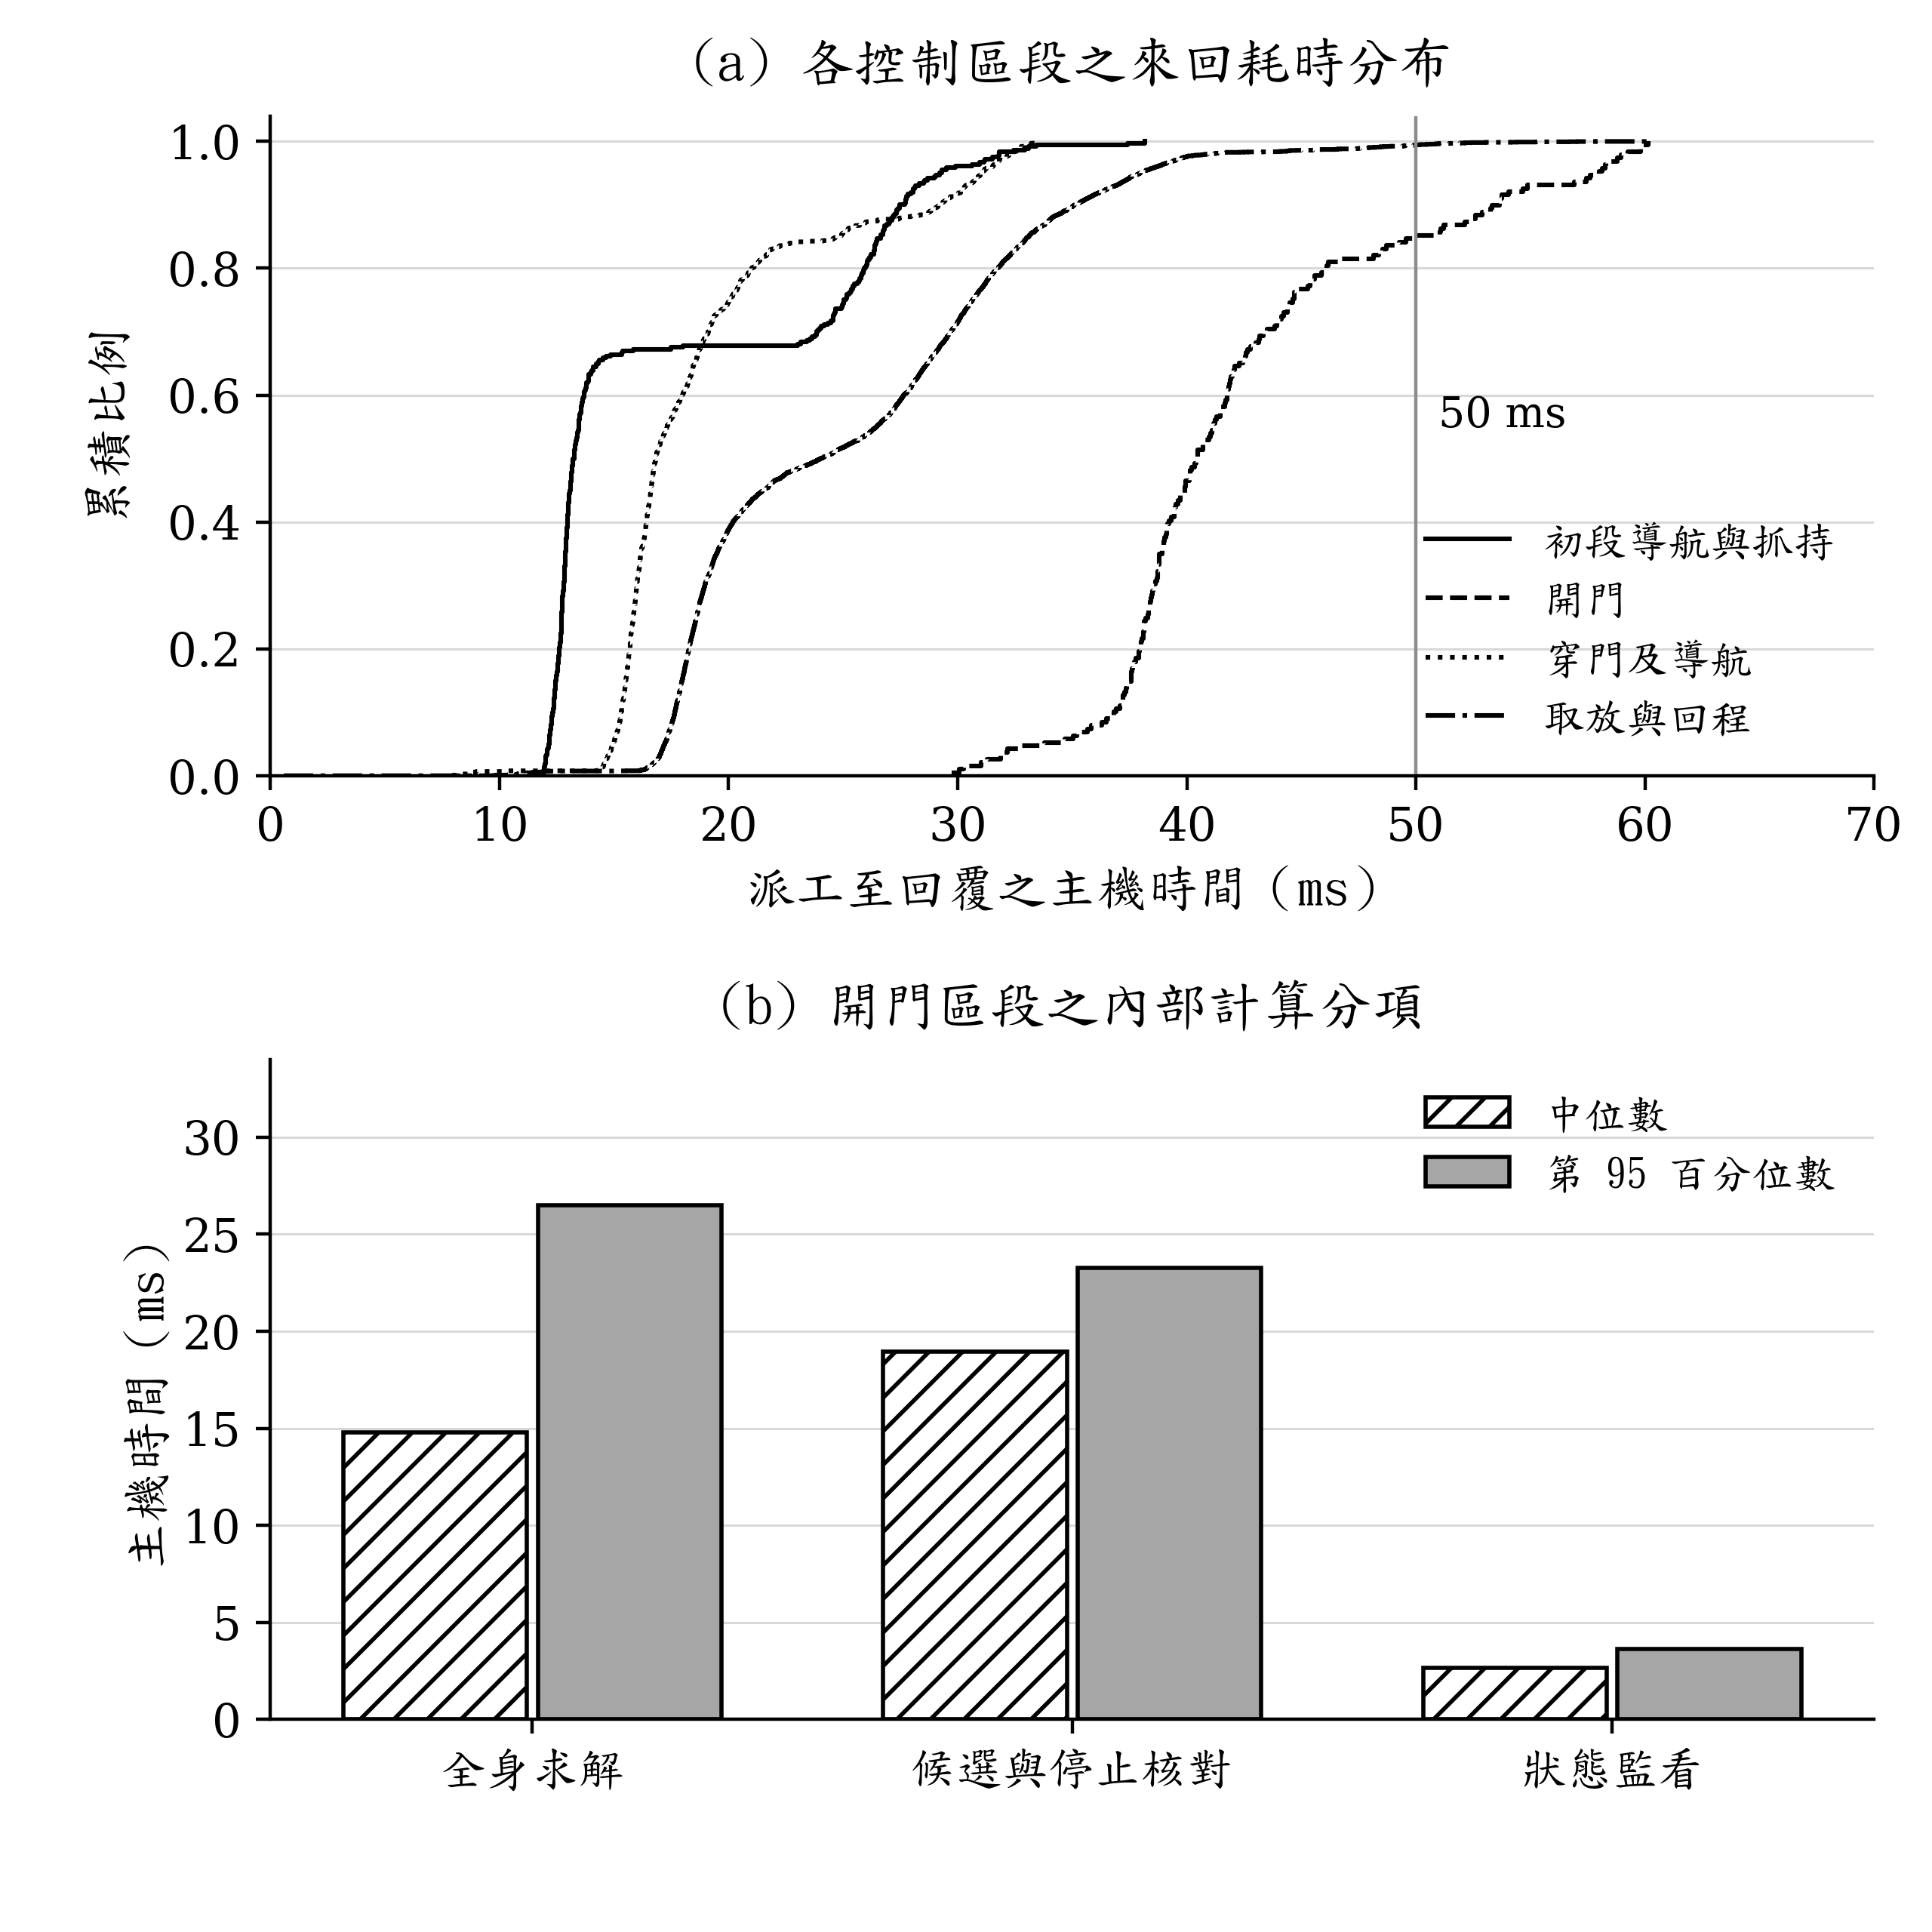
\includegraphics[width=0.98\textwidth]{figsrc/ch04/control_computation_timing.png}
    \caption{住宅代表案例之計算耗時：
    (a) 四個控制區段的來回耗時經驗累積分布，
    垂直線為一倍速 $20$ Hz 的 $50$ ms 主機週期對照；
    (b) 開門區段之全身求解、候選與停止核對及狀態監看耗時。
    各分項的中位數與第 $95$ 百分位數分別統計。}
    \label{fig:ch4_control_computation_timing}
\end{figure}

開門段的計算分項如\cref{fig:ch4_control_computation_timing}(b)所示。
全身求解、候選與停止核對及狀態監看的耗時中位數，
分別為 $14.80$、$18.95$ 與 $2.66$ ms。
在全身求解內部，矩陣組裝與 Goldfarb--Idnani 數值求解的中位數
分別約為 $8.39$ 與 $0.61$ ms。
這些分項具有包含關係，各項分位數亦分別計算，
用於辨識控制更新中主要的計算成本。
候選與停止核對需沿軌跡檢查構型與幾何條件，
其耗時在此案例中占有相當比例。

視覺處理另於背景程序執行。
保存的 $1853$ 筆分割耗時中，中位數為 $18.81$ ms，
第 $95$ 百分位數為 $24.66$ ms，最大值為 $368.24$ ms，出現在首筆紀錄。
感知更新頻率、資料年齡與控制更新頻率因此分別核對。
整段模擬器紀錄為 $371.56$ 模擬秒與 $606.0$ 主機秒，
平均實時因子約為 $0.613$，
其範圍與第 4.5 節由控制權交接事件起算的任務時間分開計算。
本組資料支持上述配速下的計算與執行結果，
一倍速連續 $20$ Hz 的控制期限仍需另行驗證。

% ==================================================
% 4.6.2 誤差來源與失敗案例分析
% ==================================================
\subsection{誤差來源與失敗案例分析}
\label{subsec:error_sources_failure_analysis}

第 4.5 節彙整的 $43$ 次紀錄中，共有 $14$ 次未完成完整住宅任務。
\cref{tab:ch4_residential_failure_categories}依各次保存的終止狀態分類，
每次紀錄僅計入一類。
此分類描述流程停止的位置及觸發條件，
個別根因仍需配合當時的狀態、輸入與幾何資料判斷。

\begin{table}[htbp]
    \centering
    \caption{住宅未完成紀錄之終止條件分類}
    \label{tab:ch4_residential_failure_categories}
    \begingroup
    \small
    \renewcommand{\arraystretch}{1.25}
    \begin{tabular}{p{0.37\textwidth} c p{0.43\textwidth}}
        \hline
        終止條件類別 & 次數 & 紀錄內容 \\
        \hline
        回覆未就緒或外層逾時 & $5$
        & 三次未於承接時取得回覆，兩次來回耗時超過預算 \\
        開門求解或內部預算中止 & $4$
        & 兩次求解失敗，兩次內部計算預算條件觸發 \\
        抽屜抓持與退出條件未達成 & $3$
        & 拉開時抓持條件失效、再次抓持逾時及退出距離不足各一次 \\
        接觸力保護中止 & $2$
        & 夾爪接觸力超過設定上限，物理模擬中止 \\
        \hline
        合計 & $14$ & \\
        \hline
    \end{tabular}
    \endgroup
\end{table}

計算相關案例顯示，外層來回時間與內部流程預算需分別處理。
兩次外層逾時的來回耗時為 $121.65$ 與 $140.60$ ms，
均超過當時的 $120$ ms 預算。
另兩次開門流程在內部耗時約 $95.1$ ms 時觸發預算條件，
其外層來回時間約為 $97$ ms，仍未取得可繼續承接的候選。
因此，單看平均耗時或外層上限，無法涵蓋所有控制段的接受條件。

操作相關案例則反映到位、抓持及退出各有獨立條件。
再次接近抽屜把手的一次紀錄中，
確認階段的雙指接觸力皆為零，最後因抓持證據逾時而停止。
另一次退出時，末端反向位移僅約 $31.5$ mm，
未達所需的 $90$ mm，故未接續後續任務。
兩次接觸力保護紀錄的峰值分別約為 $41.99$ 與 $49.18$ N，
超過設定的 $40$ N 上限。
該兩例中止後未繼續物理步進，保留當時狀態，
其後的減速與停穩過程沒有量測證據。

其餘 $12$ 次未完成紀錄曾進入停止尾段。
停穩核對要求最終命令歸零、在途輸入排清，
並連續 $0.3$ s 符合
\begin{equation}
    \|v_B\|_2<0.003\ \mathrm{m/s},\qquad
    |\omega_B|<0.003\ \mathrm{rad/s},\qquad
    \|\dot q_a\|_\infty<0.002\ \mathrm{rad/s}.
    \label{eq:ch4_measured_stopping_conditions}
\end{equation}
判定期限為最後非零輸入後的 $4$ s。
其中 $10$ 例在 $0.37$--$1.78$ s 內取得符合條件的連續區間，
另外兩例在保存的觀測期間未通過。

\cref{fig:ch4_stopping_residual_counterexamples}呈現兩個未通過案例的逐軸最大關節速率。
抽屜拉開中止與開門回覆逾時後，
最後一筆量測的最大關節速率分別約為 $5.10$ 與 $2.28$ mrad/s，
且未形成所需的連續低速區間。
停止尾段播放完成與實際機器人停穩因此分別核對，
接觸耦合、關節追蹤及殘餘運動仍是後續驗證的重要項目。

\begin{figure}[htbp]
    \centering
    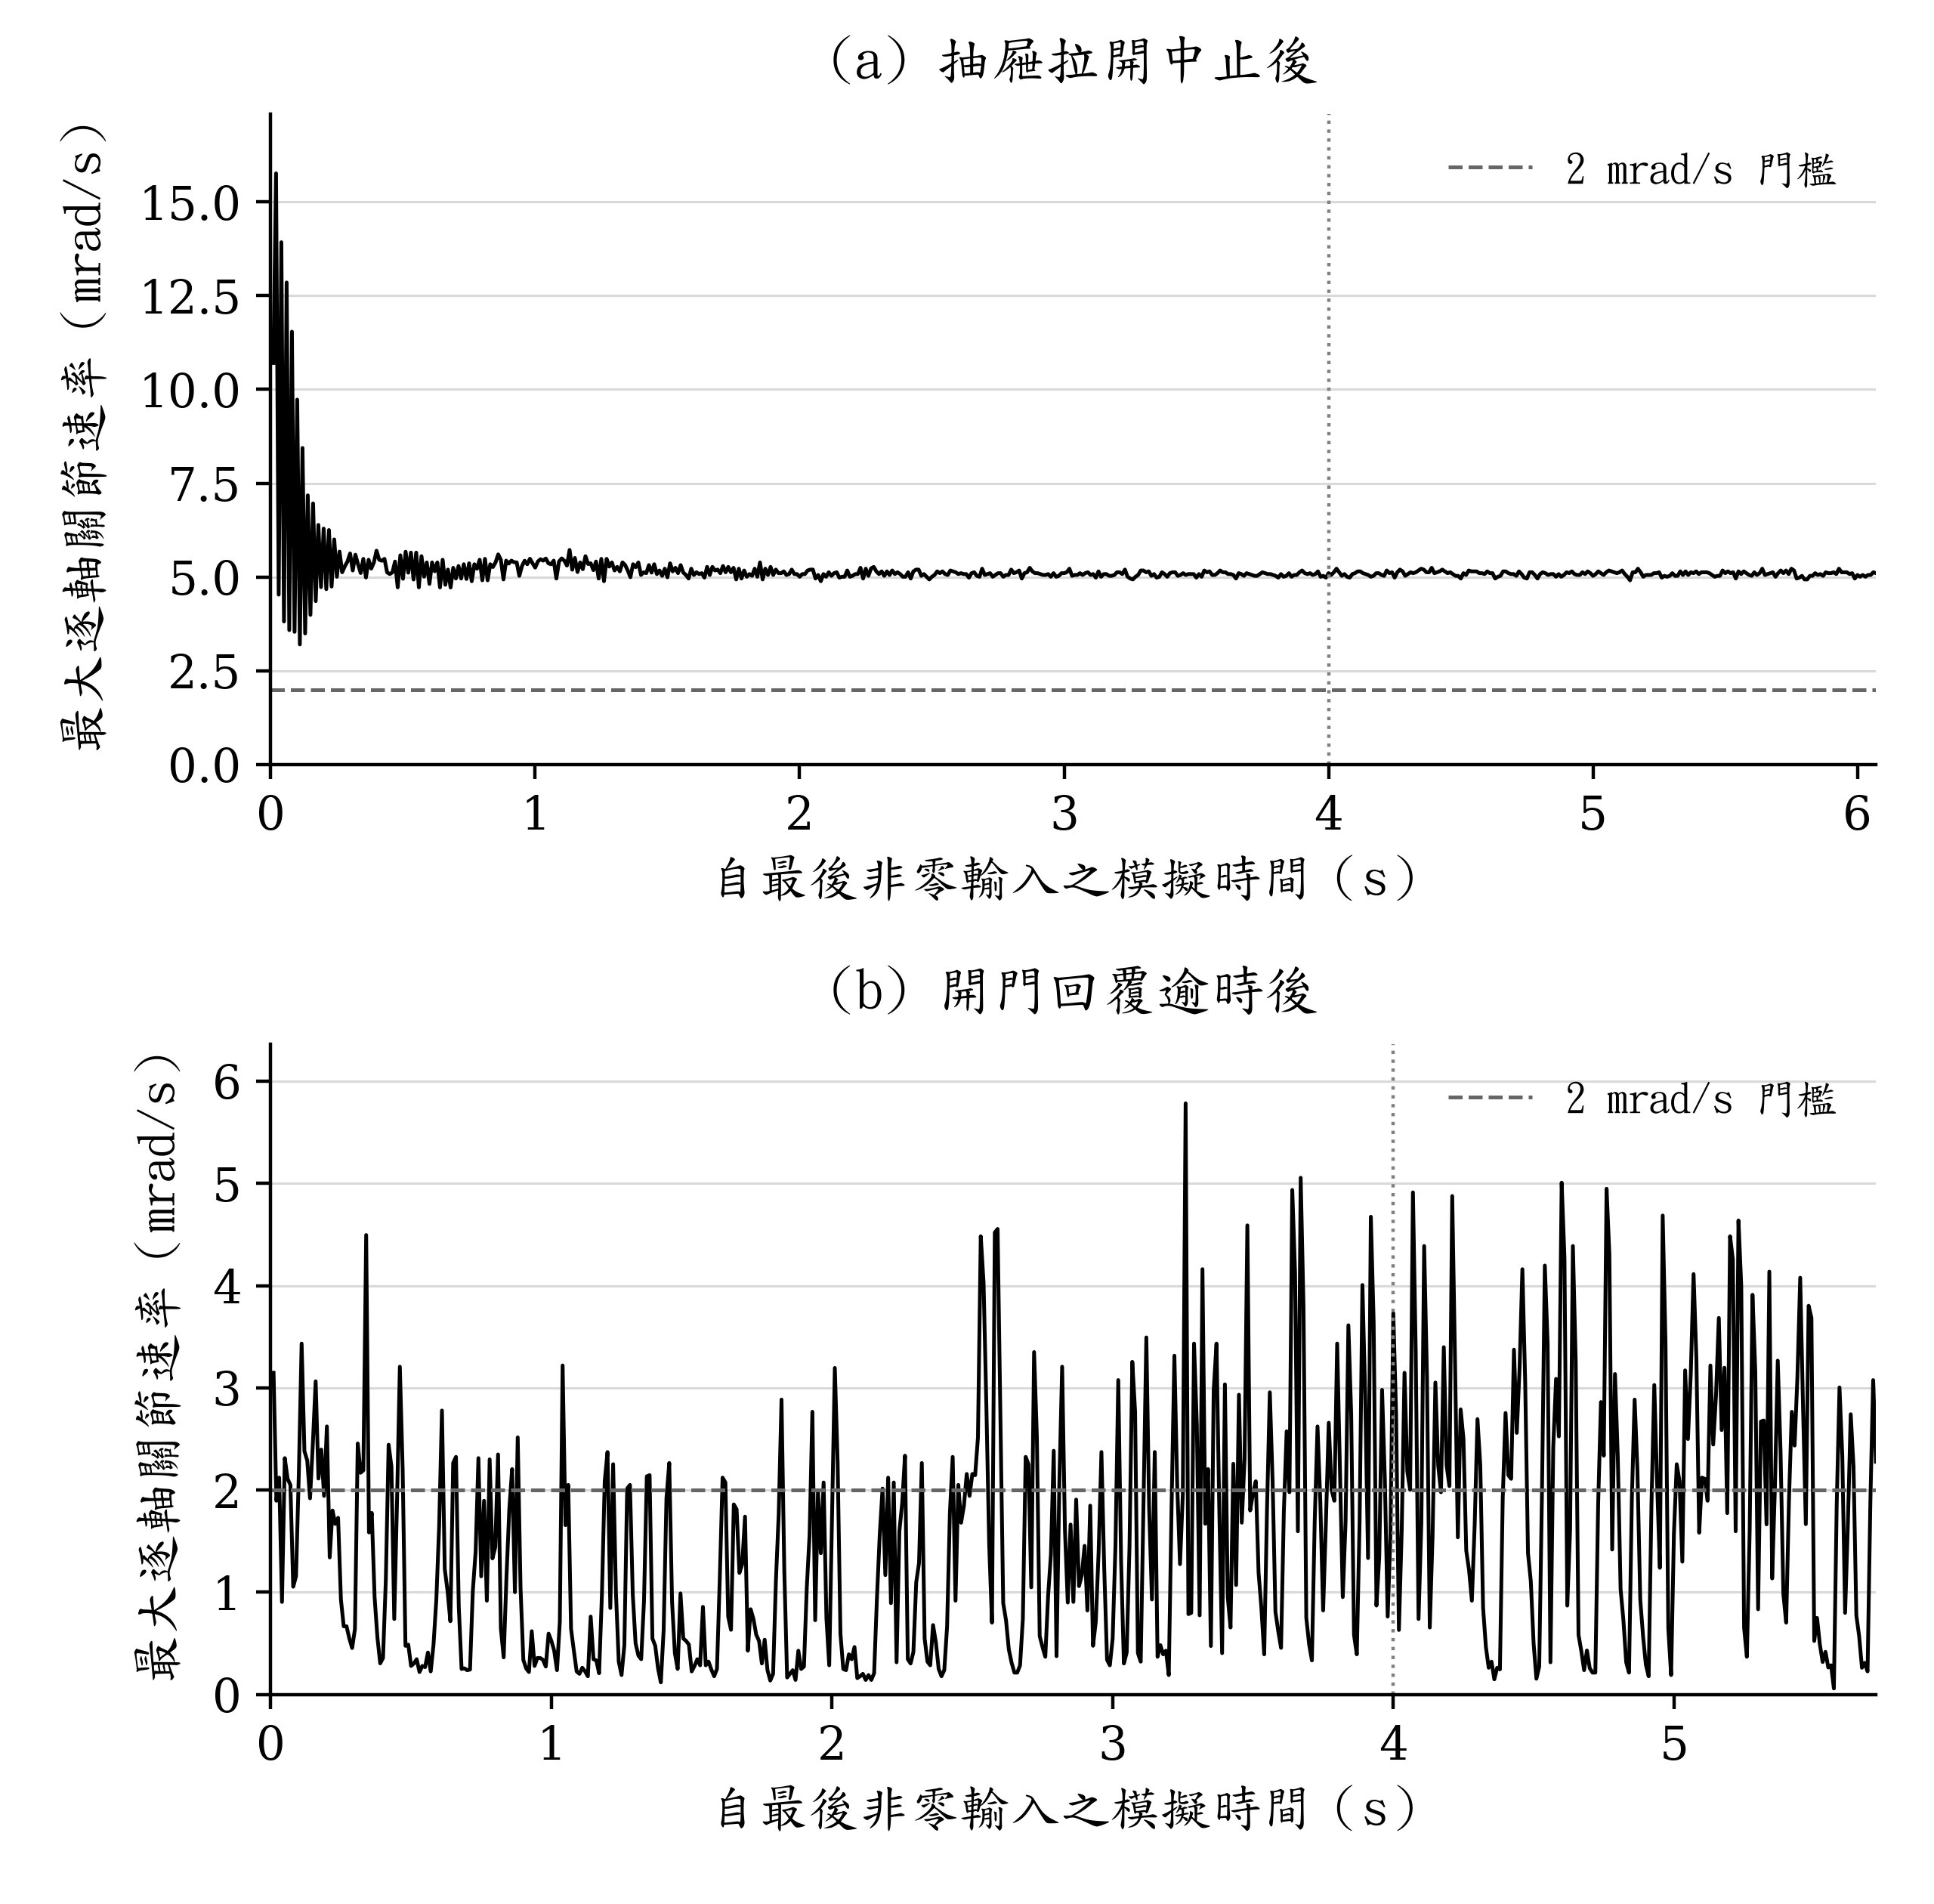
\includegraphics[width=0.98\textwidth]{figsrc/ch04/stopping_residual_counterexamples.png}
    \caption{停止尾段後未通過停穩判定的兩個案例：
    (a) 抽屜拉開中止後；(b) 開門回覆逾時後。
    曲線為每一物理步由關節位置差分取得的最大逐軸速率；
    水平虛線為 $2$ mrad/s 門檻，垂直點線為 $4$ s 判定期限。
    完整停穩條件另包含底盤速率、命令歸零及連續保持時間。}
    \label{fig:ch4_stopping_residual_counterexamples}
\end{figure}

% ==================================================
% 4.6.3 方法適用範圍與限制
% ==================================================
\subsection{方法適用範圍與限制}
\label{subsec:method_scope_limitations}

本研究的主要證據來自指定模擬場景與已配置的操作目標，
各項比較的範圍如\cref{tab:ch4_evidence_scope_limits}所示。
模型辨識與離線重播支持位置介面的預測描述，
導航與操作結果則呈現相應配置下的控制表現。
不同平台、控制版本與時間定義依前述各節分別保留。
第 4.2 節的偏置更新採固定軌跡離線重播評估；
線上偏置與末端積分補償的個別貢獻，
仍需於相同初始條件下進行獨立消融。

\begin{table}[htbp]
    \centering
    \caption{實驗證據之適用範圍與限制}
    \label{tab:ch4_evidence_scope_limits}
    \begingroup
    \small
    \renewcommand{\arraystretch}{1.25}
    \begin{tabular}{p{0.17\textwidth} p{0.35\textwidth} p{0.36\textwidth}}
        \hline
        評估面向 & 目前證據 & 適用範圍與限制 \\
        \hline
        執行模型
        & 設定點追蹤辨識、單步及多步離線重播
        & 對應辨識增益與資料條件；負載及控制介面改變時需重新驗證 \\
        導航避障
        & 共同路線到達、平面淨空與模組消融
        & 受外形近似、感測與場景規則影響；幾何重疊與實際接觸分別解讀 \\
        全身操作
        & 底盤與末端協同、抽屜與住宅任務銜接
        & 持物採固定相對位姿假設，尚未涵蓋完整摩擦抓持與滑移 \\
        視覺感知
        & 模擬 RGB-D 目標估測與時間對齊
        & 物件尺寸與家具幾何具有先驗，實體影像與感測誤差尚需驗證 \\
        計算執行
        & 設定配速下的計算耗時與停止紀錄
        & 使用分階段配速與 $120$ ms 外層預算，尚未完成一倍速控制期限驗證 \\
        任務統計
        & 配對案例與整合紀錄之完成及中止情形
        & 部分資料包含版本修正，條件時間比較限於完成案例 \\
        \hline
    \end{tabular}
    \endgroup
\end{table}

感知與定位方面，住宅模擬以物理位姿提供底盤里程，
雷射由無額外雜訊的射線量測建立，
相機轉換使用渲染時刻的機器人構型。
目前結果尚未包含實體定位漂移、相機標定誤差與影像域差異的共同影響。
物件搜尋區域、尺寸與家具機構亦具有先驗，
因此觀測導引的結果限於這些先驗與有效量測所涵蓋的範圍。

接觸與幾何方面，固定相對位姿能維持持物及閉鏈操作的運動學關係，
但摩擦不足、滑移與柔順接觸需另行建模及驗證。
筆狀物件使用粗筆代理模型，其抓取條件與細筆不同。
線上幾何核對涵蓋已啟用的機器人、家具與盒體近似，
持物外形及盒內既有物件尚未完整納入碰撞預測。
CBF 的局部線性化、鬆弛與有限步取樣，
也使實驗淨空結果限於所使用的幾何與離散檢查條件。

命令一致性方面，住宅代表案例保存了最終放行值與執行回授，
其提案對放行的檢查另記錄 $219$ 筆未配對提示及 $41$ 筆差異提示。
當時配置沿用實際放行值進行預測與執行，
上述提示以紀錄方式保留，並未全部作為中止條件。
因此，流程完成仍需配合完整的最終輸入重播，
才能進一步核對全程預測與執行的一致性。

後續驗證需先固定控制與任務配置，
補齊放行命令、停止尾段與實際運動之間的逐步對應，
再增加感測擾動、接觸條件與重複測試。
第五章依本章證據整理研究貢獻，
並提出計算期限、實體抓持與動態場景驗證的後續工作。
